\section{Deep Learning Methods in Action Recognition}
\label{sec:deep}
This section provides a detailed review of recent action recognition approaches, that are based on deep learning.
In comparison to using local spatio-temporal features, as described in section \ref{chap:conventional}, deep learning algorithms do not require hand-crafted feature engineering.
Although local spatio-temporal feature approaches yield competitive performance, the findings of \textcite{wang_evaluation_2009} indicate, that there is no universally best hand-engineered set of features for all types of datasets.
This suggests, that learning feature representation directly from the available data by using deep learning methods may be advantageous \cite{le_learning_2011}.

Similar to \cite{herath_going_2016} we categorize deep learning approaches according to the underlying method of learning feature representations from input videos.
In the case of neural network approaches, this corresponds to their architectures.
The taxonomy is shown in figure \ref{fig:deep_taxonomy}.
Leaf nodes correspond to specific approaches reviewed in this section.

\begin{figure}[H]
    \centering
    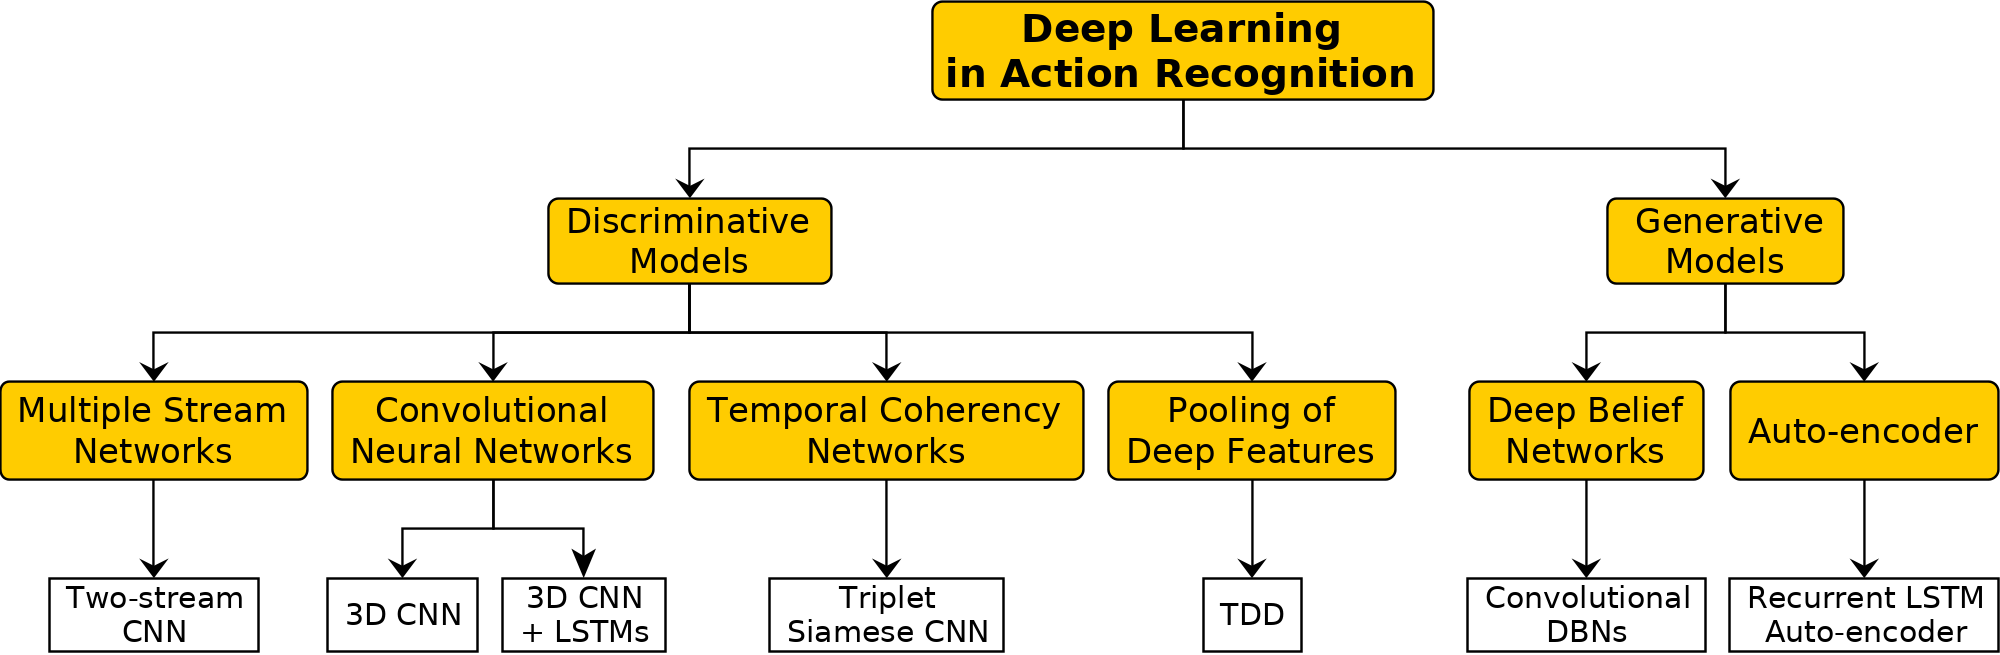
\includegraphics[width=\textwidth]{img_deep/deep_taxonomy}
    \caption{Taxonomy of Deep Learning approaches in Action Recognition.}
    \label{fig:deep_taxonomy}
\end{figure}

\textbf{Convolutional Networks}\\
Using convolutional neural networks for action recognition is motivated by their good performance on image classification tasks.
The naive approach for extending CNNs to the video domain involves applying a regular 2D CNN architecture to individual video frames and averaging the framewise class predictions over the video.
This approach however ignores motion information and therefore wastes the potential of information encoded in the temporal evolution of a an action.
3D convolutions, an extension of regular 2D convolutions, are proposed to incorporate this information from video volumes.
A video volume is constructed by stacking video frames and thereby treating the temporal dimension as an additional spatial dimension.

\textbf{Multiple Stream Networks}\\
These approaches use the decomposability of videos into a spatial component (analysing different frames) and a temporal component (analysing the change between frames) for action recognition.
They represent one of the most successfull architectures in action recognition \cite{wang_action_2015}.
The underlying principle considers, that the temporal dimension has different characteristics as the spatial dimension and should therefore be handled separately, not in a joint 3D space.
A prototypical approach of multiple stream networks is represented by the two-stream architecture \cite{simonyan_two-stream_2014}.

\textbf{Temporal Coherency Networks}\\
Temporal Coherency provides a form of weak supervision and states, that consecutive video frames are correlated semantically and dynamically \cite{herath_going_2016}.
To redescribe: adjacent video frames belonging to the same action class is likely and sudden changes in motion are rather unlikely.
By learning to classify sequences according to their temporal coherency, i.e.\ whether they are in correct or incorrect temporal order, results in learning feature representations, that encode motion information of persons and object in the sequence.
These representations can be used to perform action recognition.

\textbf{Pooling of Deeply Learned Features}\\
The prototypical approach of this category constructs \textit{Trajectory-pooled Deep Convolutional Descriptors (TDD)} \cite{wang_action_2015} for action recognition.
TDDs are obtained by applying a generic deep feature extractor around densely sampled trajectories and pooling the resulting features for each trajectory.
The approach aims at combining the advantages of hand-crafted feature methods (specifically the \textit{Improved Dense Trajectories} approach \cite{wang_action_2013}) with the expressiveness of deep architecture (specifically the \textit{Two-Stream ConvNet} approach \cite{simonyan_two-stream_2014}.

\textbf{Generative Models} are introduced in section \ref{sec:generative} below.

\subsection{Important aspects of Action Recognition Approaches}
?? TODO video representations, i.e.\ how to apply fixed length model to variable length videos.

\subsection{Convolutional Networks}

\subsubsection{3D Convolutional Neural Networks for Human Action Recognition (2010/2013)}

\textcite{ji_3d_2013} propose 3D convolutions for action recognition from video with convolutional neural networks (CNNs).
3D convolutions are able to process spatial as well as temporal information in a convolutional layer.

In regular 2D CNNs the convolutional layers apply 2D convolutional kernels to the previous layers to extract features from them.
More formally, in the notation of the authors, the value $v_{ij}^{xy}$ at spatial position $(x,y)$ of feature map $j$ in convolutional layer $i$ of the network is given by:
\begin{align*}
    v_{ij}^{xy} = \tanh \left( b_{ij} + \sum_m \sum_{p=0}^{P_i -1} \sum_{q = 0}^{Q_i - 1} w_{ijm}^{pq} v_{(i-1)m}^{(x+p)(y+q)} \right)
\end{align*}
The two inner sums over $p$ and $q$ carry out the convolutional operation on feature map $v_{(i-1)m}$ of the previous layer $i-1$ with the 2 dimensional convolutional kernel $w_{ijm}$ (spatial indices omitted).
Thereby $w$ is a tensor-like object, which contains all 2 dimensional convolutional kernels in the network, that produce feature maps through convolution
Specifically, $w_{ijm}^{pq}$ denotes the value at spatial positions $(p,q)$ of the 2D convolutional kernel, which is applied to feature map $m$ of the previous layer $i-1$.
Feature map $j$ in layer $i$ is finally obtained by summing the results of all the convolutions performed on the feature maps of layer $i-1$ over $m$, adding a bias and passing it into a non-linear function (here $\tanh(\cdot)$).

$P_i$ and $Q_i$ denote the dimensions of the kernels in $x$ and $y$-direction respectively.
The convolutional operation used here is called \textit{cross-correlation}, which differs from the mathematical discrete convolution in that the convolutional kernel is not flipped. This results in a non-commutative operation as described in chapter 9 of \cite{goodfellow_deep_2016}.

\textcite{ji_3d_2013} propose an extension of 2D convolutions by using three dimensional kernels, i.e.\ two spatial dimensions as above and an additional temporal dimension.
More formally the value $v_{ij}^{xyz}$ of feature map $j$ at spatio-temporal position $(x,y,z)$ in convolutional layer $i$ is given by:
\begin{align*}
    v_{ij}^{xyz} = \tanh \left( b_{ij} + \sum_m \sum_{p=0}^{P_i -1} \sum_{q = 0}^{Q_i - 1} \sum_{r = 0}^{R_i - 1} w_{ijm}^{pqr} v_{(i-1)m}^{(x+p)(y+q)(z+r)} \right)
\end{align*}
As above, $w_{ijm}^{pqr}$ denotes the value of the now three dimensional kernel at spatio-temporal position $(p,q,r)$, which performs convolution on the $m$th feature map of the previous layer $i-1$ to obtain feature map $j$ in convolutional layer $i$.
$R_i$ additionally denotes the dimension of the kernel in temporal direction. 

Based on 3D convolutions, the authors design a neural network architecture, that takes an input of $7$ video-frames of size $60 \times 40$ pixels.
The details of the architecture as shown in figure \ref{fig:3dconv_architecture} are described below:

\begin{figure}[H]
    \centering
    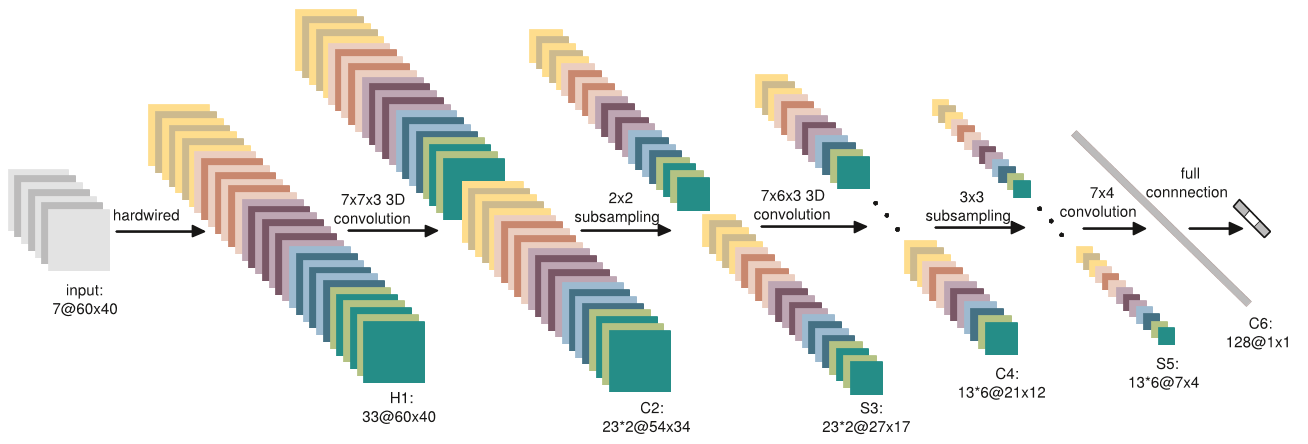
\includegraphics[width=\textwidth]{img_deep/3dconv_architecture}
    \caption{3D CNN architecture developed for human action recognition \cite{ji_3d_2013}}
    \label{fig:3dconv_architecture}
\end{figure}
The architecture contains one hard-wired layer, three convolutional layers \textit{C2, C4} and \textit{C6}, two subsampling layers for dimensionality reduction \textit{S3} and \textit{S5} and one fully connected layer for classification.

At first, hard wired connections are applied to the input frames, in order to extract gray values of the input frames, gradients along the horizontal and vertical direction and the optical flow between two consecutive frames. This results in 33 feature maps in layer $H1$, organized in five different channels: \textit{gray, gradient-x, gradient-y, optflow-x} and \textit{optflow-y}.

The first convolutional layer \textit{C2} applies two 3D kernels with dimensions $7\times7\times3$ ($7\times7$ pixels in the spatial dimension and $3$ frames in the temporal dimension) to each of the five channels in layer $H1$ separately. 
This results in $2\times5$ channels with a total of 46 feature maps in layer \textit{C2}.
The first convolutional layer therefore requires $\text{(kernel-weights)} + \text{(biases)} = 2 \times 5 \times 7 \times 7 \times 3 + 2 \times 5 = 1480$ trainable parameters. 

After subsampling layer \textit{S3}, three different 3D kernels with size $7 \times 7 \times 3$ are applied to each of the $2 \times 5$ channels of the previous layer to get the feature maps in layer \textit{C4}.
The last convolutional layer \textit{C6} performs 2D convolutions to obtain $128$ feature maps of dimension $1 \times 1$.

The resulting vector of these 128 feature maps in layer $C6$ is interpreted as a 128-dimensional feature representation of the input.
This feature representation is then classified by a fully connected layer into the required number of output classes.

In total the architecture contains $295,458$ trainable parameters, which are initialized randomly and learned by online error back-propagation as done by \textcite{lecun_gradient-based_1998-1}.
The authors tried other architectural layouts but conclude that the one described above works best.

The network is evaluated as part of an action detection and recognition system, using the TRECVID 2008 development dataset \cite{rose_trecvid_2009}.
Additionally, it's performance is measured as stand-alone approach on the KTH benchmarking datset \cite{schuldt_recognizing_2004}.

\textbf{Evaluation on TRECVID:} \\
The TRECVID 2008 development dataset \cite{rose_trecvid_2009} contains 49 hours of surveillance videos continuously recorded by five different cameras on five days at London Gatwick Airport.
The dataset is annotated for surveillance event detection, i.e.\ what events occur where.
The authors train their model to recognize three action classes from the dataset: \textit{CellToEar}, \textit{ObjectPut} and \textit{Pointing}.
The other action classes provided by the dataset were used to generate negative training examples.
The distribution of training examples sorted by date is shown in figure \ref{fig:3dconv_dataset}.
Example frames of the dataset are shown in figure \ref{fig:3dconv_sampletracking}.

\begin{figure}[H]
    \centering
    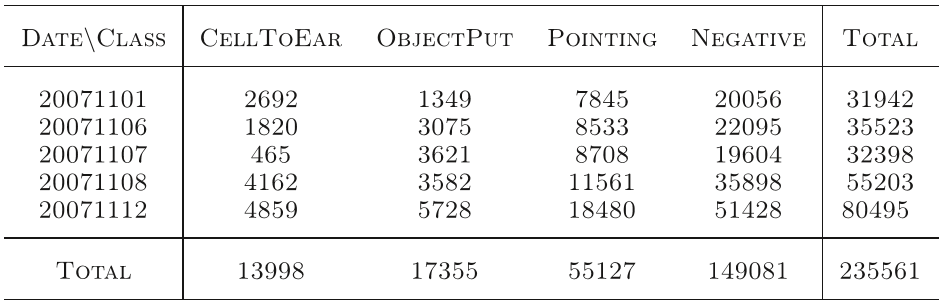
\includegraphics[width=0.75\textwidth]{img_deep/3dconv_dataset}
    \caption{Number of action samples per class from the TRECVID 2008 development dataset \cite{ji_3d_2013}}
    \label{fig:3dconv_dataset}
\end{figure}

Since the dataset provides continuous videos with several persons in a real-world scene, \textcite{ji_3d_2013} apply a human detector and a detection-driven tracker, to keep track of the heads in the scene.
This information is used to extract a bounding box around a person, as soon as an action is performed. 
Six additional bounding boxes are sampled from three frames before and three frames after the action was detected with a temporal step size of two frames.
The bounding boxes have the same size and are sampled at the same spatial location as the initial bounding box.

The contents of these 7 bounding boxes are stacked and used as input of the 3D CNN architecture in order to classify the performed action.

\begin{figure}[H]
    \centering
    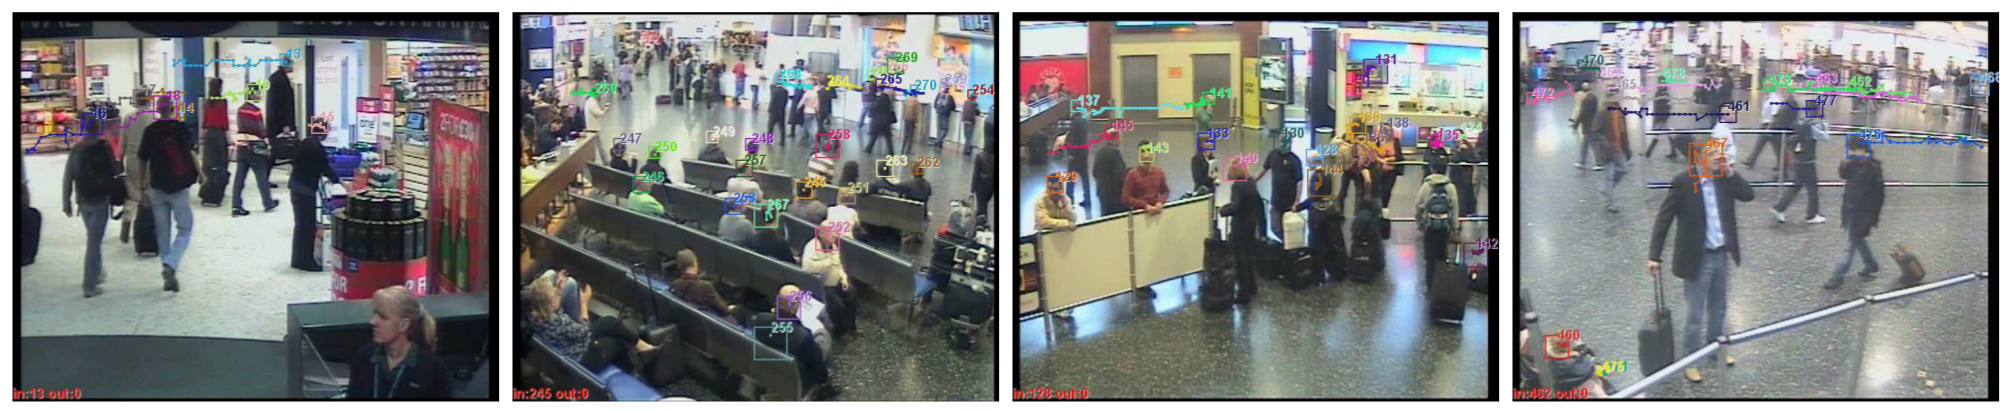
\includegraphics[width=\textwidth]{img_deep/3dconv_sampletracking}
    \caption{Example scenes of the TRECVID 2008 development dataset with results of human detection and tracking \cite{ji_3d_2013}}
    \label{fig:3dconv_sampletracking}
\end{figure}

To evaluate the performance of the 3D CNN model, the authors compare it to three other baseline approaches in the detection and recognition system:
\begin{enumerate}
    \item A frame-based 2D CNN model, which averages the action class predictions over individual frames.
    \item Extraction of dense SIFT features \cite{lowe_distinctive_2004} from the seven gray scaled input frames, which are then aggregated using the BoW-Paradigm and classified through a linear SVMs.
    \item Extraction of dense SIFT features \cite{lowe_distinctive_2004} from motion edge history images (MEHI)\cite{yang_human_2009} of the input frames, which are then aggregated as above.
\end{enumerate}

The 3D CNN model outperforms the other approaches on the TRECVID 2008 development dataset significantly for all classes except \textit{Pointing}, where the 2D frame-based CNN performed best.
The authors note, that the number of training examples for \textit{Pointing} are significantly larger than for any other class and conclude, that their architecture performs best, when few positive examples are present.

\textbf{Evaluation on KTH:}\\
Furthermore, the stand-alone 3D CNN architecture was evaluated on the KTH dataset \cite{schuldt_recognizing_2004}.
It achieves an overall accuracy of $90.2\%$ on that benchmark.
In comparison: \textcite{schindler_action_2008} achieved $92.7\%$ and \textcite{jhuang_biologically_2007} achieved $91.7\%$ several years earlier.

\textcite{ji_3d_2013} showed, that 3D convolutions yield competitive performance compared to state-of-the-art approaches at that time as shown on the KTH benchmark \cite{schuldt_recognizing_2004}.
Although the authors reference the work of \textcite{schindler_action_2008} which states, that 5-7 video-frames are enough for recognizing simple actions, this short temporal extend is often identified as a deficit of the approach and addressed in following approaches, e.g.\ by \textcite{baccouche_sequential_2011}.


\subsubsection{Sequential Deep Learning for Human Action Recognition (2011)}
\textcite{baccouche_sequential_2011} identify two deficits of previous approaches for extending CNNs to the video domain, specifically the approach of 3D convolutions such as \cite{ji_3d_2013} and \cite{kim_human_2007}:
\begin{enumerate}
    \item They still rely on hand crafted inputs (hard wired pre-processing of the data to produce image gradients and optical flow in the first processing layer).
    \item The models typically process less than 15 input frames, and therefore only classify short sub-clips, not the entire video.
\end{enumerate}

To address these issues, the authors design a two-step deep architecture, which is shown in figure \ref{fig:sequentialdeep_overview} and consists of:
\begin{enumerate}
    \item A convolutional spatio-temporal feature extractor network, based on 3D convolutions.
    \item A recurrent neural network (RNN) classifier, which incorporates LSTM cells \cite{hochreiter_long_1997} to classify the entire sequence of previously extracted spatio-temporal features.
\end{enumerate}

\begin{figure}[H]
    \centering
    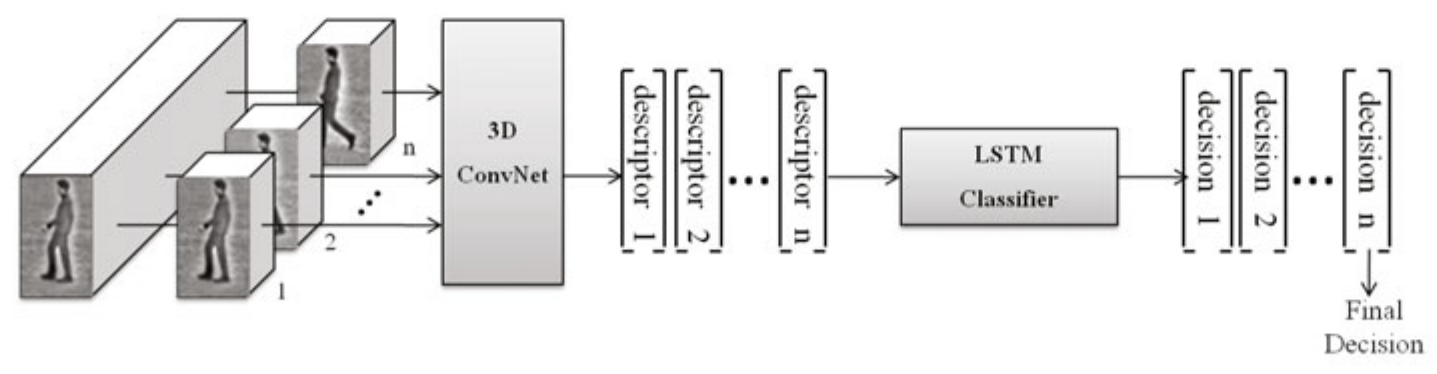
\includegraphics[width=\textwidth]{img_deep/sequentialdeep_overview.png}
    \caption{Overview of the two-step architecture consisting of a 3D ConvNet and a recurrent neural network classifier. \cite{baccouche_sequential_2011}}
    \label{fig:sequentialdeep_overview}
\end{figure}

\textcite{baccouche_sequential_2011} incorporate the work of \textcite{ji_3d_2013} by using a 3D ConvNet as feature extraction stage, which processes raw pixel values instead of hand-crafted inputs.
To compensate the problem of temporally short inputs and to take the temporal evolution of movements during an action into account, a RNN classifier is added, because they are able to process input sequences of arbitrary length.
The RNN classifies a sequence of feature representations, previously extracted by applying the 3D ConvNet to temporally adjacent patches of the input video, in order to recognize an action. 
Similarly to \cite{ji_3d_2013}, the overall approach is evaluated on the KTH dataset \cite{schuldt_recognizing_2004}.

Details of the 3D ConvNet architecture are shown in figure \ref{fig:sequentialdeep_cnnarchitecture}.
\begin{figure}[H]
    \centering
    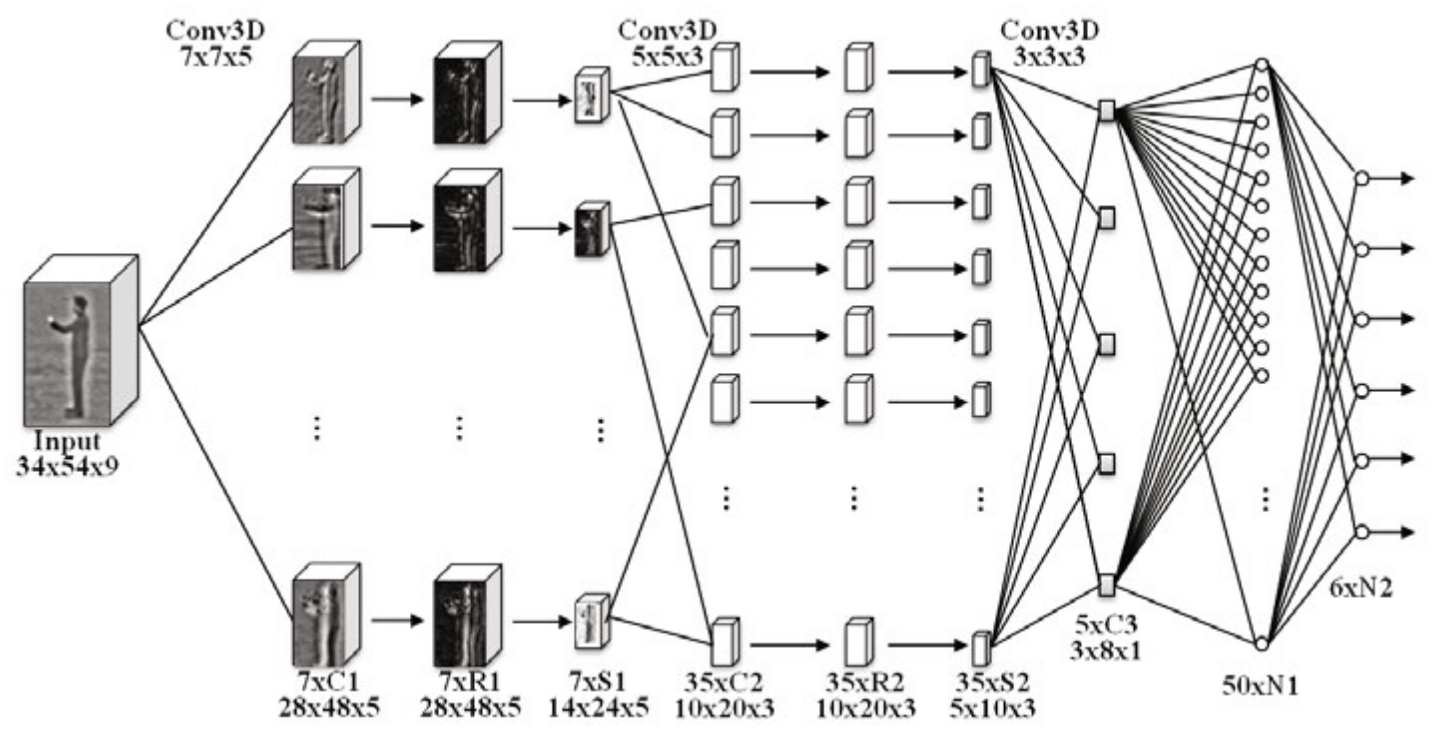
\includegraphics[width=0.9\textwidth]{img_deep/sequentialdeep_cnnarchitecture}
    \caption{Detailed architecture of the 3D ConvNet for later use with an RNN classifier. \cite{baccouche_sequential_2011}}
    \label{fig:sequentialdeep_cnnarchitecture}
\end{figure}

The input to the 3D ConvNet is formed by stacking $9$ successive frames from the input video of spatial resolution $34\times54$ pixels.
The network contains three convolutional layers \textit{C1, C2} and \textit{C3}.
The first two convolutional layers are followed by rectification and subsampling layers \textit{R1, S1} and \textit{R2, S2}.
A rectification layer simply computes the absolute value of its input \cite{baccouche_sequential_2011}.
The third convolutional layer is followed by two neuron layers (fully-connected layers) \textit{N1} and \textit{N2}.

The ConvNet model, as shown in figure \ref{fig:sequentialdeep_cnnarchitecture} embeds $17,169$ trainable parameters in total, which is about 15 times less than the $295,458$ parameters used by \textcite{ji_3d_2013}.

Specifically, the layers are configured as follows:
\begin{enumerate}
    \item Convolutional layer \textit{C1} computes $7$ feature maps, by convolving $7$ 3D $7\times7\times5$ kernels with the stacked input frames.
    \item Layer \textit{R1} and \textit{S1} perform rectification (building of the absolute value) and subsampling with a spatial factor of 2 respectively.
    \item Convolutional layer \textit{C2} computes $35$ feature maps (the $7$ feature maps in layer \textit{S1} are connected to two different convolutional kernels, which results in $14$ feature maps and pairs of different feature maps in \textit{S1} are connected to one convolutional kernel each, which results in additional $21$ feature maps, summing to a total of $35$ feature maps).
    \item Convolutional layer \textit{C3} computes $5$ features maps, which are fully connected to all feature maps in previous layer \textit{S2} by $3\times3\times3$ convolutional kernels. These five feature maps have dimension $3\times8\times1$, rendering the raw input encoded as a 120 dimensional feature vector.
\end{enumerate}

The 3D ConvNet is trained individually on the KTH dataset before employing the RNN classifier.
For training, the 120 dimensional feature vector is fed into two fully connected layers \textit{N1} and \textit{N2} with 6 output neurons, one for each class of the KTH dataset.
The authors use the same training algorithm as \textcite{ji_3d_2013}: online backpropagation with momentum adapted to weight-sharing.

For training the RNN classifier with online backpropagation through time \cite{gers_learning_2002}, the fully connected layers \textit{N1} and \textit{N2} of the 3D ConvNet are removed.
The 120 output values of the third convolutional layer \textit{C3} are fed into the recurrent neural network as input at each time step.
Several configurations were tested by the authors and a single hidden layer with 50 LSTM cells were found to be a good compromise between training time and performance.
The LSTM cells are fully connected to the outputs of layer \textit{C3}.

The authors find their 3D ConvNet model alone, without adding the recurrent LSTM classifier, to yield a recognition rate of $91.04\%$ on KTH, when the classification is done by majority voting over several short sub-sequences of the test-video.
This result is comparable to other approaches at that time and almost the same as obtained by \textcite{ji_3d_2013} ($90.2\%$), although the model requires about 15 times less parameters.
When using the LSTM classifier network, recognition performance increases to $92.17\%$.


\subsubsection{Large-scale Video Classification with Convolutional Neural Networks (2014)}
\textcite{karpathy_large-scale_2014} provide a comprehensive examination of techniques to apply convolutional neural networks to the domain of action recognition from video.
More specifically, their contribution is four-fold:
\begin{enumerate}
    \item They gather the Sports-1M dataset containing a collection of 1 million automatically annotated sports videos from YouTube (further described in section \ref{chap:datasets} of this work).
    \item They evaluate several approaches besides three dimensional convolutions for extending CNNs to process spatio-temporal data in a consistent and therefore comparable manner. These methods are called \textit{fusion methods} in the phrasing of the authors, since temporal motion information has to be fused with spatial motion information while propagating through a network.
    \item They propose a generic multi-resolution convolutional architecture in oder to speed up training time at no cost in accuracy.
    \item They retrain the top layers of a network on the UCF-101 dataset, which has previously been trained on the Sports-1M dataset and thereby achieve a significant increase in performance against training the network on UCF-101 alone (transfer learning).
\end{enumerate}

The authors first implement a baseline CNN architecture, which classifies human action videos by processing a single frame at a time, i.e.\ without considering temporal relationship between frames.
Based on the single frame architecture, several extensions for processing temporal information in the network are being investigated. These types of fusion methods are depicted in figure \ref{fig:largescale_fusionmethods}.

\begin{figure}[H]
    \centering
    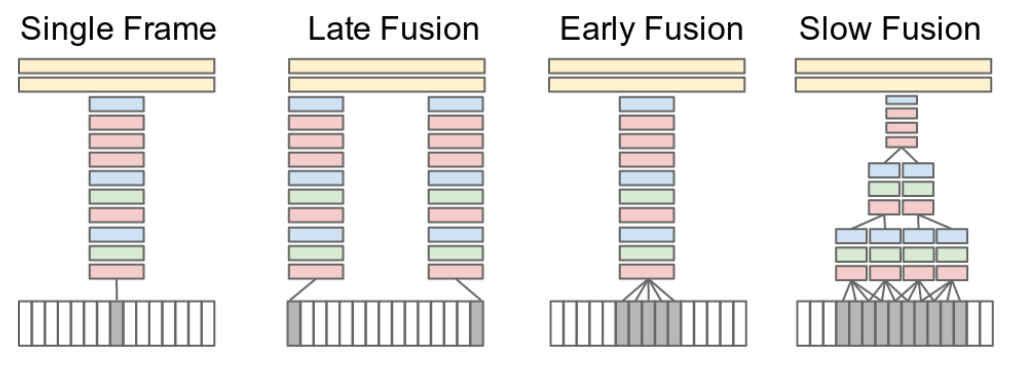
\includegraphics[width=0.75\textwidth]{img_deep/largescale_fusionmethods}
    \caption{Different methods for fusing temporal with spatial information in convolutional neural network architectures. Red, green and blue denotes convolutional, normalization and pooling-layers. Grey colored inputs are single RGB video frames. Yellow layers are fully-connected for classification. \cite{karpathy_large-scale_2014}}
    \label{fig:largescale_fusionmethods}
\end{figure}

\textbf{Single Frame}\\
The CNN model used in the single frame approach is a deep convolutional neural network with 2D convolutions, that recognizes actions by classifying frames of a given input sequence individually and reporting the averaged prediction.
The architecture is similar to AlexNet, which won the 2012 ImageNet Classification Challenge \cite{krizhevsky_imagenet_2012-1}, but receives slightly smaller inputs: $170\times170\times3$ instead of $224\times224\times3$ in the ImageNet model.
The first two dimensions thereby correspond to the spatial resolution of the video, the third dimension to the RGB color channels of a video-frame.
This approach is evaluated as a baseline in order to measure the improvement when using temporal information, i.e.\ several frames, in the recognition process. 

\textbf{Early Fusion}\\
In the early fusion approach temporal information is incorporated in the network on the pixel level by extending the convolutional kernels in the first layer to be of dimension $11 \times 11 \times 3 \times T$, where $T$ is the temporal extend, i.e.\ the number of input frames to the network.
The authors set $T = 10$ which corresponds to a third of a second.
Note that the temporal information is completely flattened after the first convolutional layer, since the kernel has the same temporal dimension as number of inputs frames.
Therefore only the kernels in the first convolutional layer are three dimensional in nature.

\textbf{Late Fusion}\\
In the late fusion methods, two separate single-frame networks with shared parameters and without their individual classification layers are used on input frames with a temporal distance of $15$ frames.
Two shared fully connected layers then merge the individual network's information and classify the input. 
The fully connected layers are able to compute motion information by comparing the feature representations of the two single-frame networks.

\textbf{Slow Fusion}\\
Temporal information is processed throughout the network by extending the kernels of each convolutional layer in time, as done in the first layer of the \textit{Early Fusion} approach.
Thereby higher layers progressively process more temporal information along the input frames.
The \textit{Slow Fusion} approach applies 3D convolutions as done by \textcite{ji_3d_2013} and \textcite{baccouche_sequential_2011}.
The first convolutional layer incorporates a temporal extend of $T = 4$ in its kernels, while the second convolutional layer uses a temporal extend of $T = 2$.
This allows the third convolutional layer layer to access the information of all 10 input frames.

\textbf{Evaluation on the Sports-1M dataset}\\
The recognition performance of the different fusion methods is evaluated on the Sports-1M dataset.
The authors use downpour stochastic gradient descent \cite{dean_large_2012} for training the models in a distributed way on a computing cluster.
For the evaluation $70\%$ of the dataset were used as training data, $10\%$ as validation set and $20\%$ as test set.

To obtain fixed-sized inputs for the models, the authors interpret an entire video as a set of short, fixed-sized video clips.
At test time, 20 short clips are sampled from the current test-video and each clip is presented to the network individually.
Each clip is passed through the network 4 times, each time using different crops and flips and the result is averaged to produce a robust class prediction.
The video-level predictions (examples shown in figure \ref{fig:largescale_classification}) are computed from the clip-level predictions simply by averaging.

\begin{figure}[H]
    \centering
    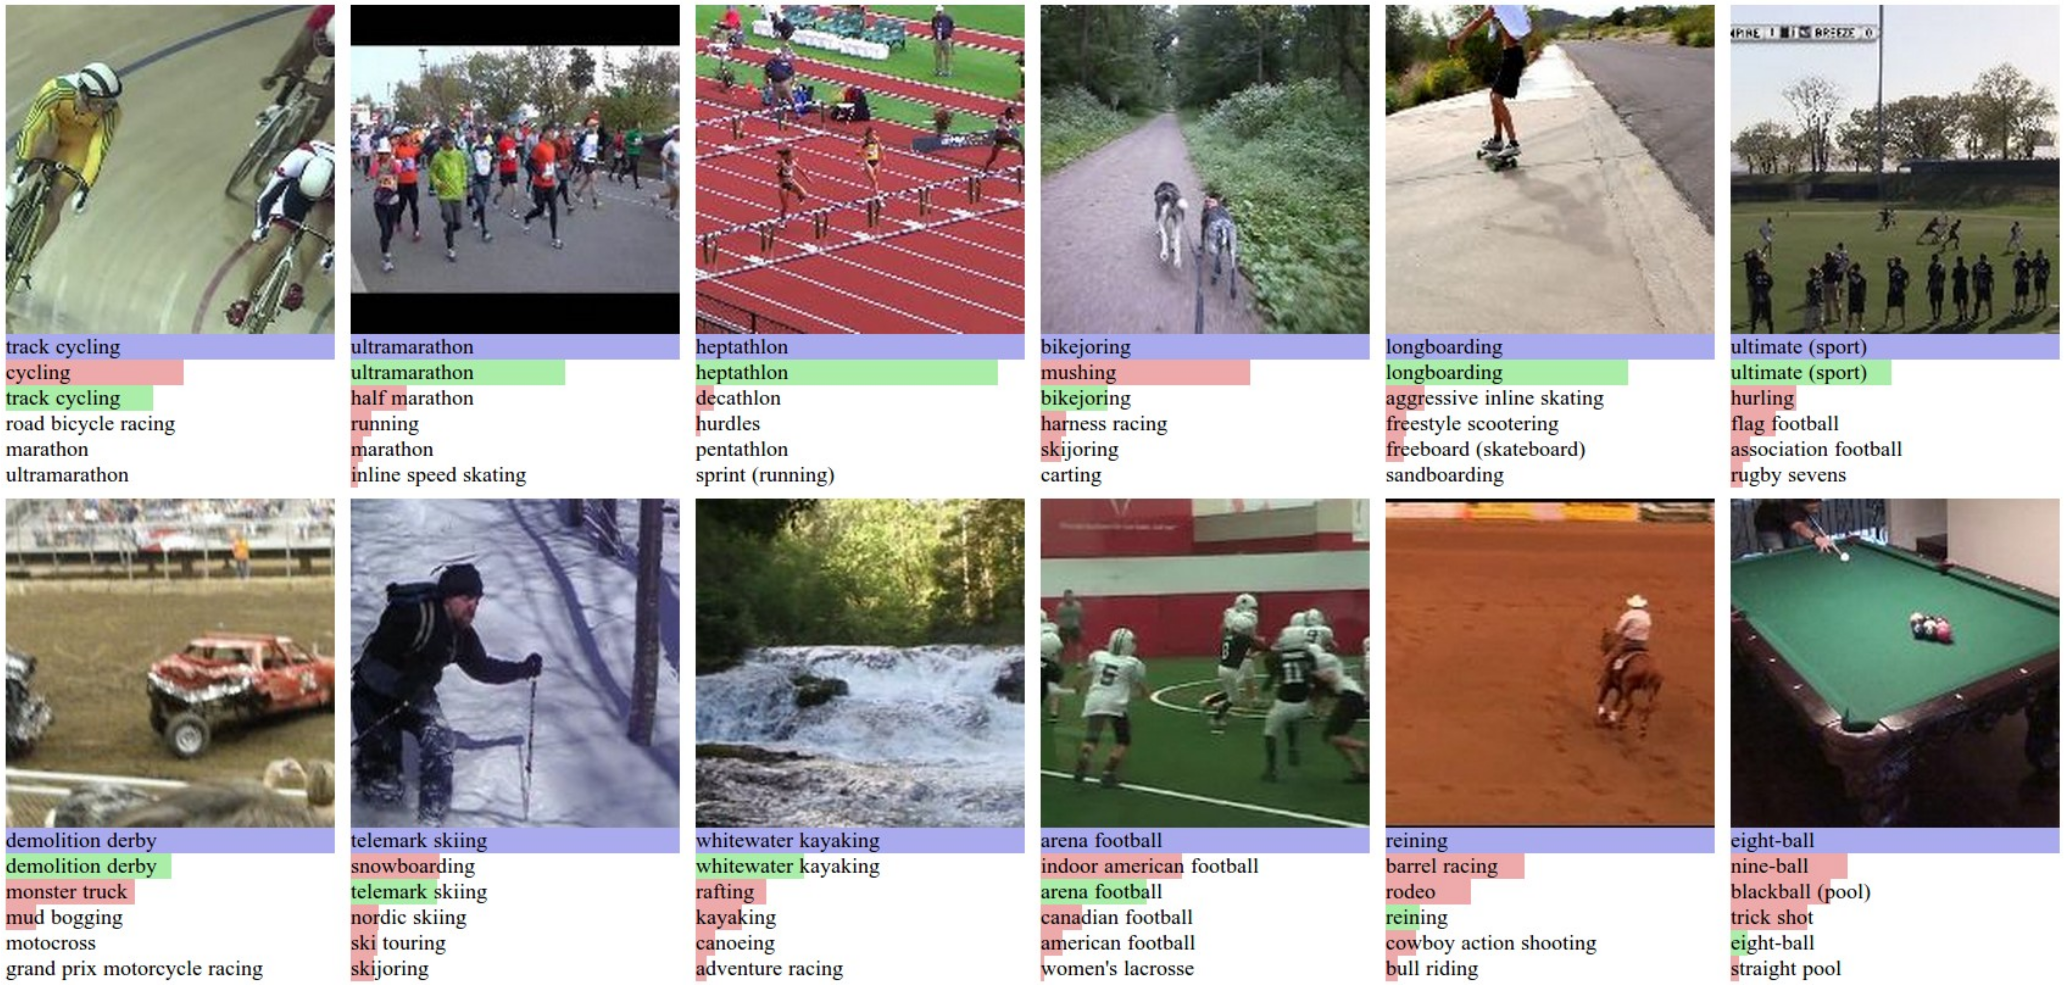
\includegraphics[width=\textwidth]{img_deep/largescale_classification}
    \caption{Classification of videos in the Sports-1M dataset. Blue label is the ground truth, below class predictions are shown with decreasing confidence. \cite{karpathy_large-scale_2014}}
    \label{fig:largescale_classification}
\end{figure}

In addition to comparing different fusion methods, the authors also implement a hand-crafted feature baseline approach, that extracts multiple kinds of hand-crafted local features from each video and aggregates them according to the bag-of-words paradigm.
The resulting feature histogram representations are classified into action classes using a multilayer neural network, with rectified linear activation units.

The performance of the studied approaches is shown in table \ref{tab:largescale_results}:
\begin{table}[H]
    \centering
    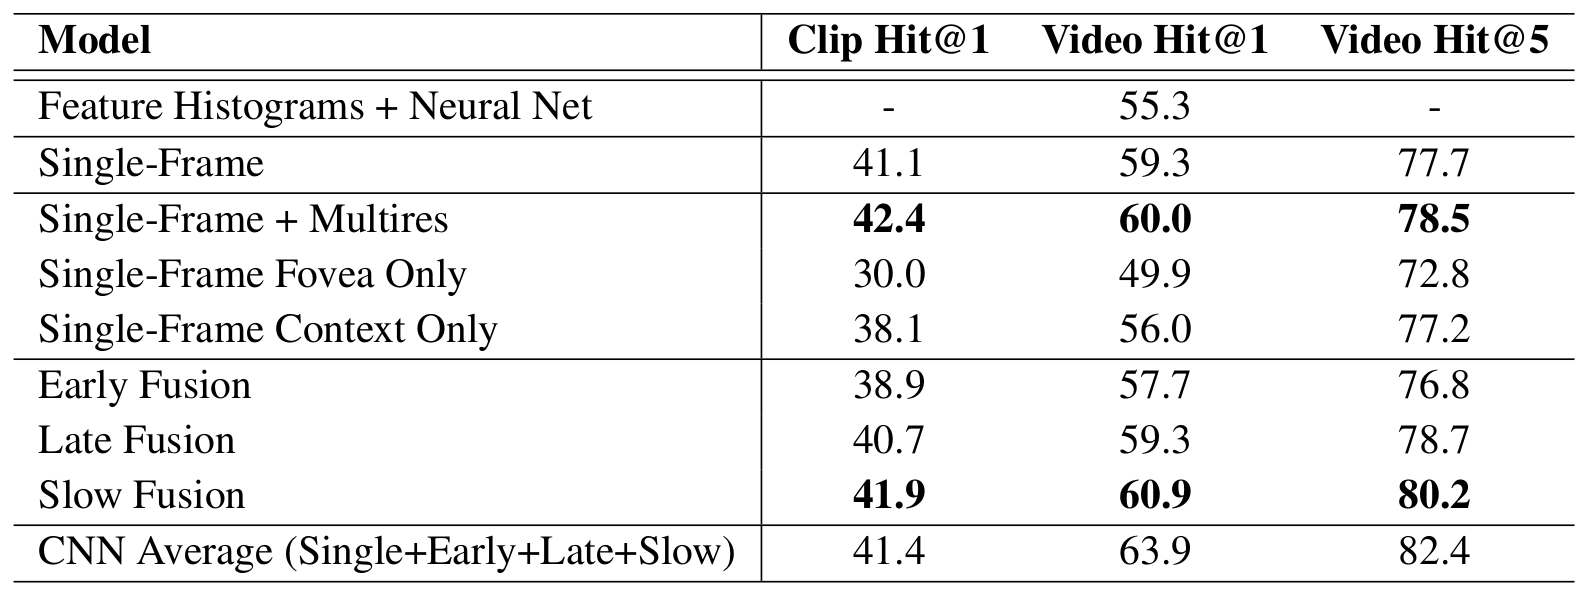
\includegraphics{img_deep/largescale_results}
    \caption{Results of different architectures on the Sports-1M dataset. Hit@$k$ denotes the percentage of test samples, that had at least one of their class labels included in the top $k$ predictions. \cite{karpathy_large-scale_2014}}
    \label{tab:largescale_results}
\end{table}

The results show, that the deep models (\textit{early}, \textit{late} and \textit{slow-fusion}) consistently outperform the hand-crafted feature baseline.
Compared to each other, the deep models perform similarly well, despite their different convolutional architectures.
The \textit{slow fusion} model, that uses 3D convolutions in all convolutional layers, outperforms the other fusion approaches by a small margin.
\textcite{karpathy_large-scale_2014} describe the performance difference of between fusion models as ``surprisingly insignificant''\cite{karpathy_large-scale_2014}.
The single-frame model performs noticeably well on it's own.
The authors suspect, that the motion aware networks suffer from camera movements such as translations or zoom.

Since the training time of a network heavily influences the amount of evaluations that can be conducted using different hyperparameter settings, it is of great interest to reduce the training time for neural networks, which lies in the in the order of weeks for CNNs\cite{karpathy_large-scale_2014}, while maintaining accuracy.

The authors therefore propose a multi-resolution architecture, that is shown in figure \ref{fig:largescale_multiresolution}.
\begin{figure}[H]
    \centering
    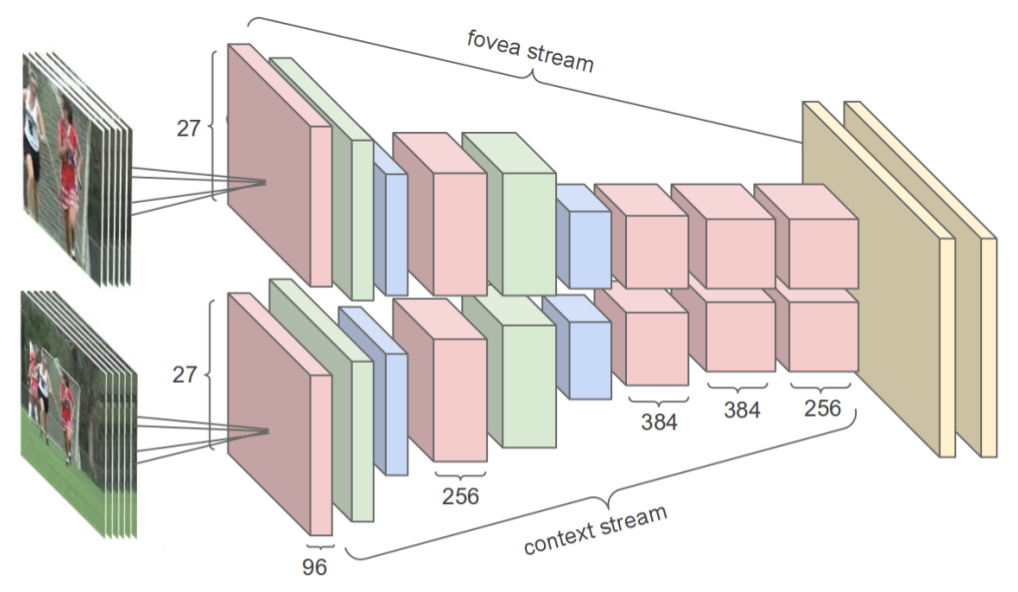
\includegraphics[width=0.75\textwidth]{img_deep/largescale_multiresolution.png}
    \caption{Multi-resolution CNN architecture \cite{karpathy_large-scale_2014}}
    \label{fig:largescale_multiresolution}
\end{figure}

The multi-resolution network processes input videos with a resolution of $178\times178$ pixel.
The context stream receives a downsampled version of the input frames, which contain the complete field of view but have a decreased resolution of $89\times89$ pixel.
The fovea stream works on just the $89\times89$ pixel sized center of the original input frames.
Both streams are implemented as the same CNN architecture and the outputs of both streams are fed into two fully connected layers, where their information is merged and a class prediction is calculated.

The input dimensionality of the multi-resolution architecture is decreased by a factor of $2$ compared to processing the raw $178\times178$ pixel input video in one stream.
The authors achieved a reduction in training time by a factor of 2-4, while maintaining the accuracy of the system (see table \ref{tab:largescale_results}).


\subsubsection{Learning Spatiotemporal Features with 3D Convolutional Networks (2015)}
\textcite{tran_learning_2015} create a generic spatio-temporal feature extractor, by training a very deep 3D ConvNet on the large-scale action recognition dataset Sports-1M \cite{karpathy_large-scale_2014}.
Given a human action video as input, the activations of the ConvNet's last fully connected layer form a descriptive feature vector, which represents the input.
The authors show, that the extracted feature representation, which they call \textit{C3D}, is generic enough to be reused on other vision tasks without requiring task-specific fine tuning of the model.
Merely a classifier (the authors use linear SVMs) has to be trained on the extracted \textit{C3D} features, given a video-based vision task.
The approach is evaluated for action recognition, action similarity labeling (ASLAN, see section \ref{chap:datasets} of this work), scene classification and object recognition.

Using a model based on 3D convolutions for \textit{C3D} is motivated by the recent review of fusion methods, published by \textcite{karpathy_large-scale_2014}, which showed that using 3D convolutions in all convolutional layers of a CNN performs best for action recognition (\textit{Slow Fusion}).  
The authors conclude that 3D convolutions preserve temporal information along the processing stages of a deep CNN, because they result in a 3 dimensional feature map.
In contrast 2D convolutions the temporal relations among frames after each convolutional layer by only processing frames spatially.
This is illustrated in following figure \ref{fig:c3d_2dconv3dconv}.
\begin{figure}[H]
    \centering
    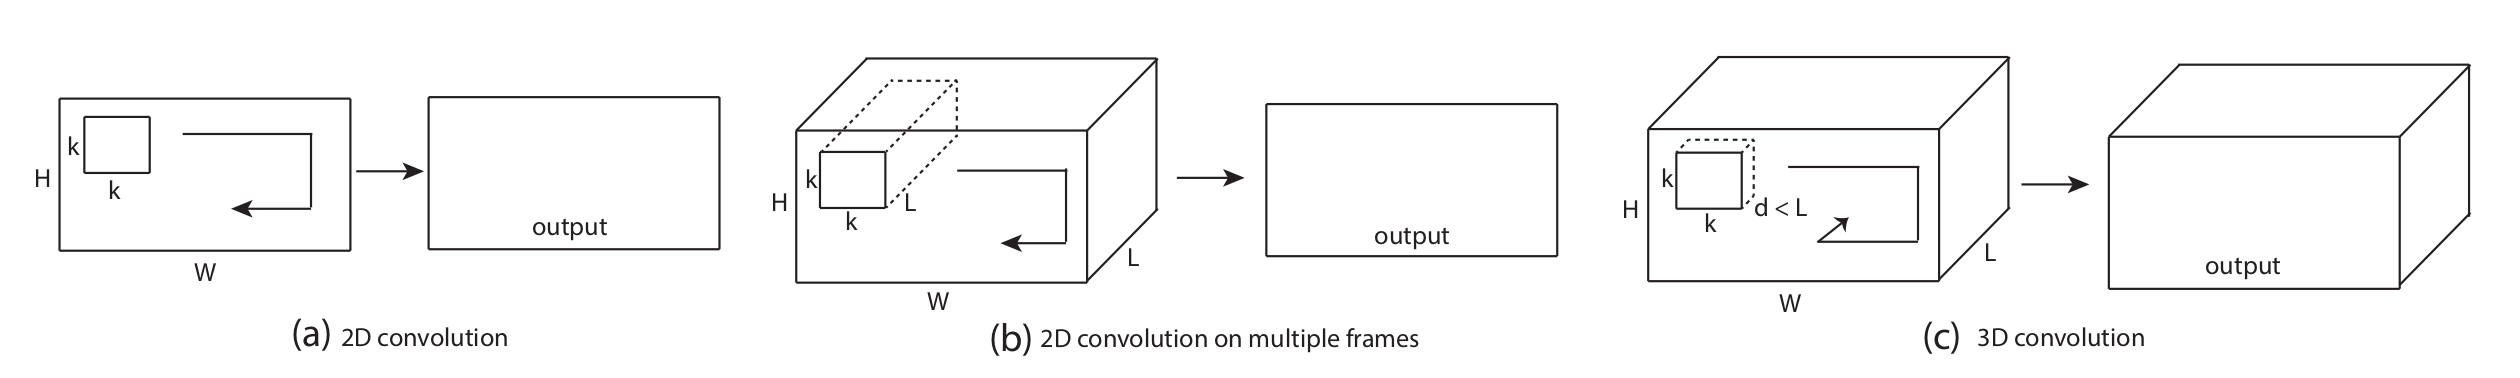
\includegraphics[width=\textwidth]{img_deep/c3d_2dconv3dconv}
\caption{Dimensionality of convolutions: a) 2D convolution on a single image results in a 2D feature map. b) 2D convolution on multiple frames, interpreted as different channels of the input, results in a 2D feature map because results of individual frames are summed. c) 3D convolution on multiple frames results in a 3D feature map, therefore preserving the temporal dimension \cite{karpathy_large-scale_2014}}
    \label{fig:c3d_2dconv3dconv}
\end{figure}

All networks take inputs of dimension $128\times171\times16$ (\textit{frame width} $\times$ \textit{frame height} $\times$ \textit{number of frames}, in three color channels each).
To find the best performing architecture, the authors first perform experiments on the medium-scale dataset UCF-101 \cite{soomro_ucf101:_2012}, because using a large-scale dataset would be too time-consuming.
More specifically, the network architecture for performing these experiments is designed as follows:
\begin{itemize}
    \item 5 convolutional layers with 64, 128, 256, 256 and 256 filters respectively.
    \item Each convolutional layer is followed by a max-pooling layer with filter size $2\times2\times2$ (except for the first layer, which has a filter size of $1\times2\times2$ for not collapsing the temporal information too early).
    \item Two fully connected layers with 2048 neurons each at the end and an additional softmax layer with one output per action class for training.
\end{itemize}

The work of \textcite{simonyan_very_2014}, regarding 2D convolutional neural networks, suggests that $3\times3$ convolutional kernels yield best results in deep architectures .
The authors therefore fix the spatial kernel size in their 3D convolutions to $3\times3$ and vary the temporal depth of the kernel $d$.
For finding the best parameter, the depth $d$ is varied according to the following two methods, results are shown in figure \ref{fig:c3d_temporaldeptheval}:
\begin{enumerate}
    \item Homogeneous temporal depth: The kernels across all convolutional layers have the same temporal depth. Four networks are evaluated with $d \in \{1, 3, 5, 7\}$.
    \item Varying temporal depth: The temporal depth changes across the convolutional layers. Two schemes are being evaluated. Increasing temporal depth $3-3-5-5-7$ and decreasing temporal depth $7-5-5-3-3$.
\end{enumerate}

\begin{figure}[H]
    \centering
    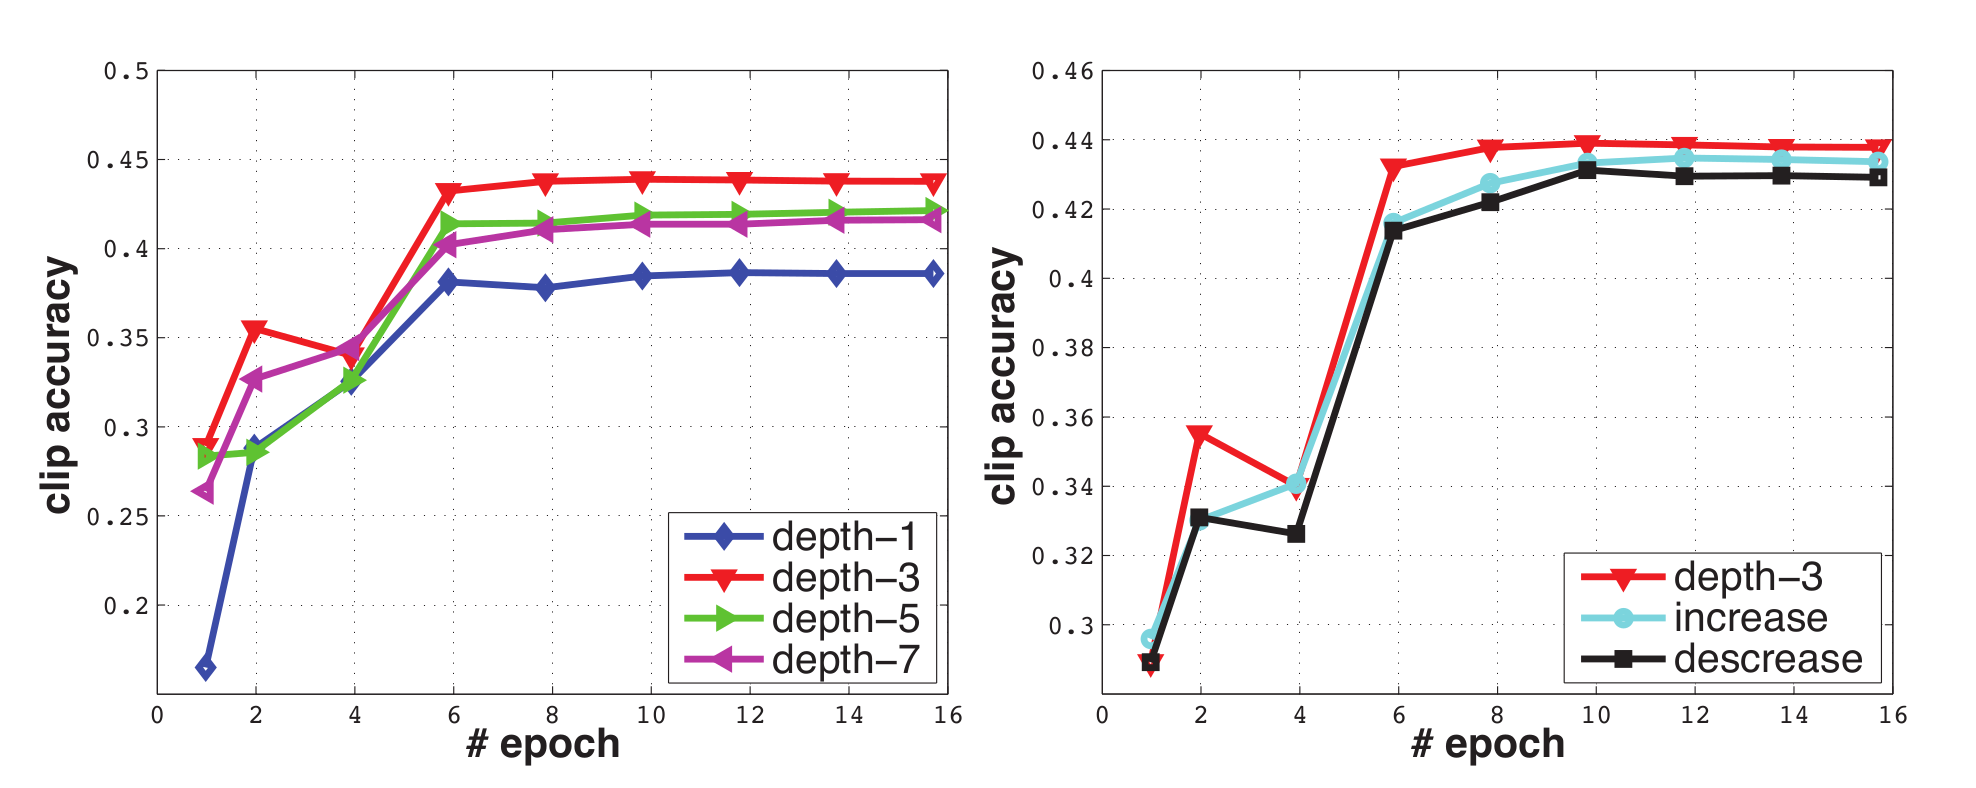
\includegraphics[width=\textwidth]{img_deep/c3d_temporaldeptheval}
    \caption{Clip accuracy for different temporal kernel depths over training epochs on UCF101. Left shows homogeneous temporal depth, right shows varying temporal depth. \cite{tran_learning_2015}}
    \label{fig:c3d_temporaldeptheval}
\end{figure}

The results indicate, that a fixed temporal depth of 3 performs best among all tested settings.
Testing a spatial kernel resolution of $5\times5$ with the same variations for $d$ yielded the same result.
The authors therefore conclude that $3\times3\times3$ kernels are the best choice in 3D convolutional networks.

The final architecture for extracting C3D features with $3\times3\times3$ convolutional kernels is constructed as follows:
8 convolutional layers, 5 pooling layers, two fully connected layers and a softmax output layer.
With 8 convolutional layers and 15 layers in total (without counting the softmax output-layer, as illustrated in figure \ref{fig:c3d_architecture}), it is the deepest architecture reviewed for the action recognition task in this work.
\begin{figure}[H]
    \centering
    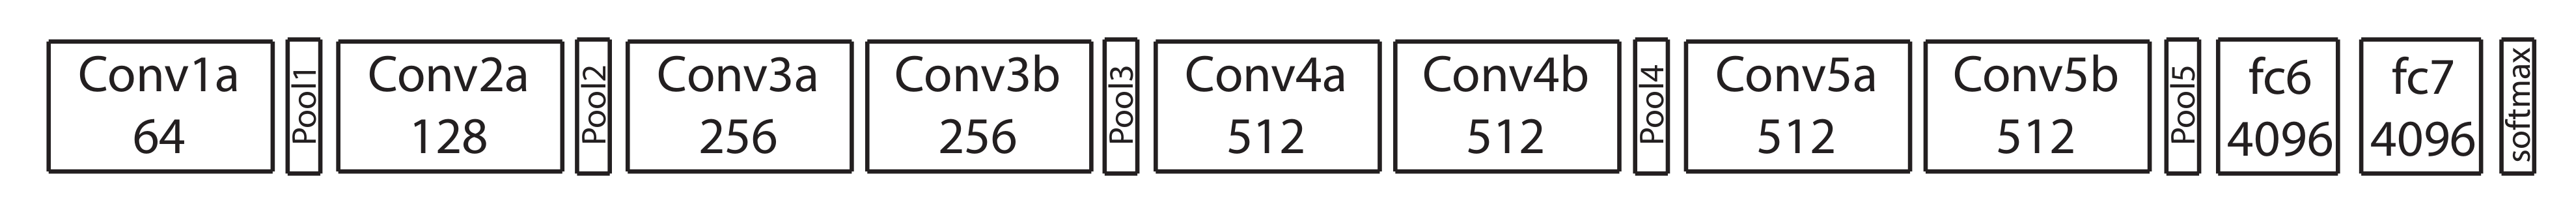
\includegraphics[width=\textwidth]{img_deep/c3d_architecture}
    \caption{C3D architecture. Number of filters is given in each box. \cite{tran_learning_2015}}
    \label{fig:c3d_architecture}
\end{figure}

\textbf{Training} The network is trained on the Sports-1M \cite{karpathy_large-scale_2014} dataset to learn spatio-temporal features.
Five two second long clips are extracted randomly from every training video and resized to a resolution of $128\times171$ pixel.
From these five clips, training inputs for the network of size $112\times112\times16$ are randomly extracted.
Training is conducted with stochastic gradient descent with batch size of 30.

\textbf{Testing} For testing, i.e.\ classification of unseen videos from the test set, video clips are extracted from a test video as during training.
A single crop of the center of a video-clip is passed through the network to obtain a clip-classification.
For obtaining video-classifications, the classifications of 10 clips are being averaged.

The \textit{C3D} approach yields video hit@5 accuracy on the Sports-1M dataset of $84.4\%$ and video hit@1 accuracy of $60.0\%$.
The authors also try to boost the performance by pre-training the model on an internal dataset (called I380K) and fine-tuning on Sports-1M, which results in a hit@5 accuracy of $85.5\%$.

Additionally, the performance of \textit{C3D} features was evaluated on UCF-101, which results in an accuracy of 82.3\% when applying a single \textit{C3D} network.
Combining the extracted features of three networks before classifying them increases the accuracy to 85.2\%.

Note, that these results were obtained by using a simple linear SVM classifier on top of the \textit{C3D} features.
Results can be improved by applying more sophisticated aggregation schemes \cite{tran_learning_2015}.

To promote the usage of \textit{C3D} features, the authors forked from the Caffe framework \cite{jia_caffe:_2014}, extended it for handling three dimensional convolutional networks and therein provide a pre-trained \textit{C3D} network model for public use.
The usage of \textit{C3D} features is therefore simple and effective, since a trained model is publicly available and the forward pass in neural networks is computationally fast.


\subsubsection{Long-term Temporal Convolutions for Action Recognition (2016)}
\textcite{varol_long-term_2016} address, similar to \textcite{baccouche_sequential_2011}, the common deficit in recent CNN extensions to action recognition of class labels being learned from very short video subsequences only.
Most often a temporal extend of only 1-16 input frames can be processed by the architectures at a time. \cite{ji_3d_2013}\cite{karpathy_large-scale_2014}\cite{tran_learning_2015}

Instead of using a recurrent neural network for classifying convolutionally extracted spatio-temporal features, as done by \textcite{baccouche_sequential_2011}, \textcite{varol_long-term_2016} study the effects of increasing the number of input frames to a 3D convolutional architecture in the context of action recognition from video.
The authors name their approach long-term temporal convolutions and their contribution is two-fold:
\begin{enumerate}
    \item A systematical evaluation of the influence of the number of input frames $T = \{20, 40, 60, 80, 100\}$ on the performance of a 3D CNN architectures.  
    \item A demonstration of the importance of high-quality optical flow inputs, in order to learn accurate video features with a 3D CNN architecture.
\end{enumerate}

Processing an increased temporal extend has to be compensated with a decreased spatial resolution, in order to not exceed computational limitations.
The studied architectures therefore process spatial resolutions of $58\times58$ or $71\times71$ pixel only.
The used 3D CNN architecture is shown in figure \ref{fig:longterm_architecture}.
$T$ therein denotes the temporal extent, i.e.\ the number of input frames to the ConvNet, and architectural details are given below.

\begin{figure}[H]
    \centering
    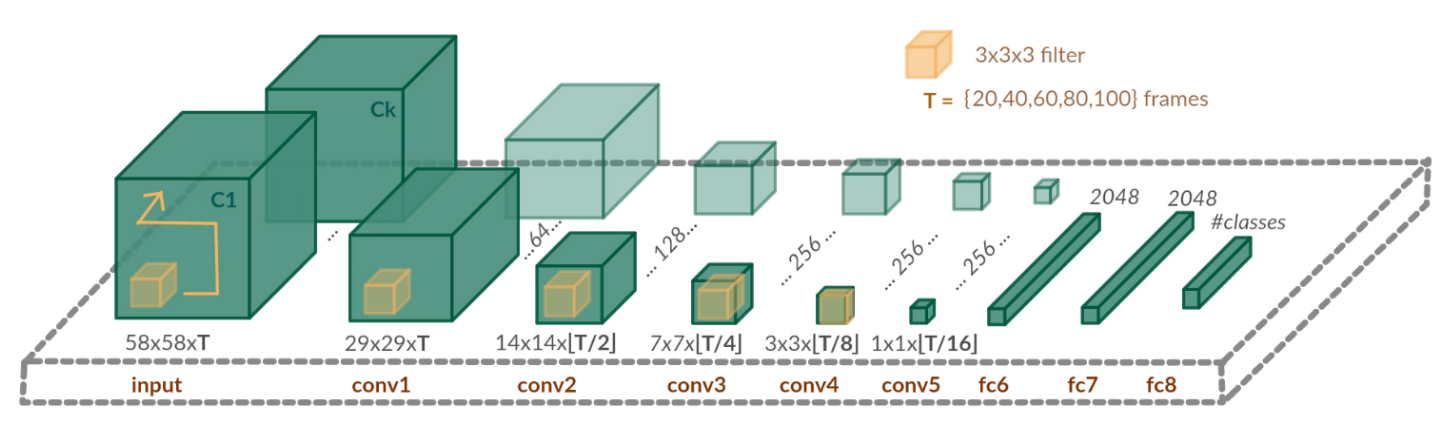
\includegraphics[width=\textwidth]{img_deep/longterm_architecture}
    \caption{3D CNN architecture for evaluating the influence of the number of input frames on action recognition accuracy. \cite{varol_long-term_2016}}
    \label{fig:longterm_architecture}
\end{figure}

\begin{itemize}
    \item 5 convolutional layers \textit{conv1}, \ldots, \textit{conv5}, that apply 3D convolutions to their previous layers and contain 64, 128, 256, 256 and 256 feature maps respectively.
    \item Kernel size of $3\times3\times3$ in each convolutional layer.
    \item After each convolutional layer: One layer of rectified linear units (ReLUs) and one layer of max-pooling with filter size $2\times2\times2$ except in the first layer where it is $2\times2\times1$ (not shown in the figure).
    \item Three fully connected layers as classifier with sizes 2048, 2048 and number of classes.
    The fully connected layers also use rectified linear units as activation function and an additional softmax layer at the end of the network.
\end{itemize}

As a baseline approach the authors first evaluate their architecture with inputs of size $112\times112\times16$, that is a spatial resolution of $112\times112$ and $T=16$ input frames, because it can be directly compared to the work of \textcite{tran_learning_2015}.
Additionally, the baseline is implemented with $T=60$ frames inputs, specifically using an input dimension of $58\times58\times60$, to provide an initial comparison between 16 and 60 frames (spatial resolution is decreased to remain computationally tractable).

The two baseline models are used to study the influence of different input modalities, network settings and data augmentation techniques such as: optical flow inputs, \textit{dropout}\cite{srivastava_dropout:_2014}, \textit{random clipping} and \textit{multiscale cropping} (explained below).

At first the influence of using optical flow as input is evaluated, specifically stacked optical flow images from the following sources:
\begin{enumerate}
    \item MPEG flow \cite{kantorov_efficient_2014}, which directly can be obtained from the video encoding. It is a fast method compared to regular optical flow estimators, but has low spatial resolution and is not available for every video frame.
    \item Farneback optical flow estimator \cite{farneback_two-frame_2003}, which is fast, but calculates noisy flow fields.
    \item Brox optical flow estimator \cite{brox_high_2004}, which generates high quality optical flow fields but is slower than the other two methods.
\end{enumerate}

Example flow estimation of a given RGB video frame for all three methods is illustrated in figure \ref{fig:longterm_optflow} (left).
The table on the right of figure \ref{fig:longterm_optflow} shows the action recognition accuracy of the 60 frame baseline network, when using optical flow or pure RGB frames as input.
Results are obtained on UCF-101 (split 1).

\begin{figure}[H]
    \centering
    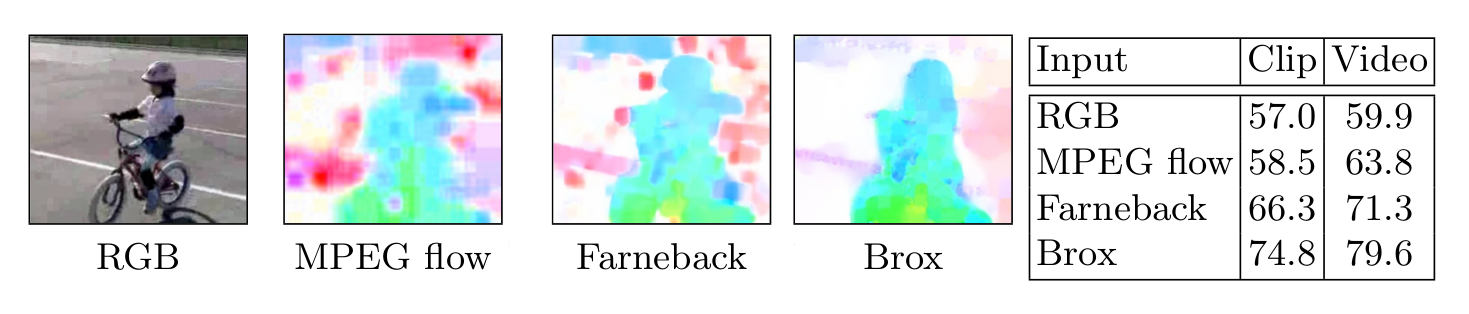
\includegraphics[width=\textwidth]{img_deep/longterm_optflow}
    \caption{Optical flow estimation of different algorithms and corresponding results when used as input for the 60 frame baseline network. Color encodes the direction of the optical flow field. \cite{varol_long-term_2016}}
    \label{fig:longterm_optflow}
\end{figure}

The results show, that high quality optical flow can boost the action recognition performance by nearly 20\% against using raw RGB video frames.
Even using low quality MPEG flow outperforms regular RGB inputs.
The authors therefore conclude, that using high quality optical flow as input is critical for learning competitive human action features from video.

Training inputs can generated by sampling video subsequences with the desired spatial and temporal dimensions from input videos at random spatio-temporal locations.
The authors call this form of pre-processing \textit{random clipping}.

The baseline approach is using a sliding-window approach with $75\%$ overlaps to generate fixed length video-clips.

An additional method for pre-processing suitable network inputs during training is called \textit{multiscale cropping}.
Input volumes, which are smaller than needed, are cropped from the training videos and then rescaled to fit to the input dimensions of the network.
The size of the crop is determined by random factors for frame width and height, sampled from $\{1.0, 0.875, 0.75, 0.66\}$.
Additionally, the scaled input is flipped with a probability of 50\%.

\textit{Dropout} \cite{srivastava_dropout:_2014} can be used during training independently of the selected cropping method.

Accuracy results for using the pre-processing methods \textit{random clipping}, \textit{multiscale cropping} and \textit{dropout} are shown in table \ref{tab:longterm_preprocessing} below.
Best performance is obtained when combining the two methods with a high dropout rate.
\begin{table}[H]
    \centering
    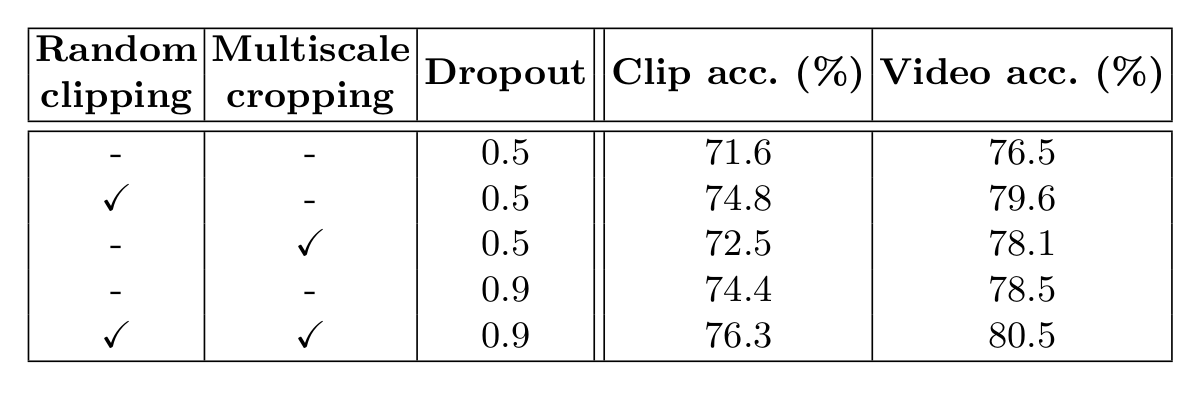
\includegraphics[width=0.75\textwidth]{img_deep/longterm_preprocessing}
    \caption{Evaluation of pre-processing methods and dropout on a 60 frame input network, trained on UCF-101 (split1) from scratch using Brox optical flow as input \cite{varol_long-term_2016}}
    \label{tab:longterm_preprocessing}
\end{table}

The two baseline architectures, which differ in the number of input frames, are evaluated on the UCF-101 dataset.
In all experiments \textit{random clipping} is used.
Results are reported in table \ref{tab:longterm_16vs60} for RGB and optical flow inputs as well as optional \textit{multiscale cropping} and different dropout ratios.
The results show that long-term temporal convolutions, as present in the 60 frame network, persistently outperform the 16 frame counterpart with a smaller temporal extent.

\begin{table}[H]
    \centering
    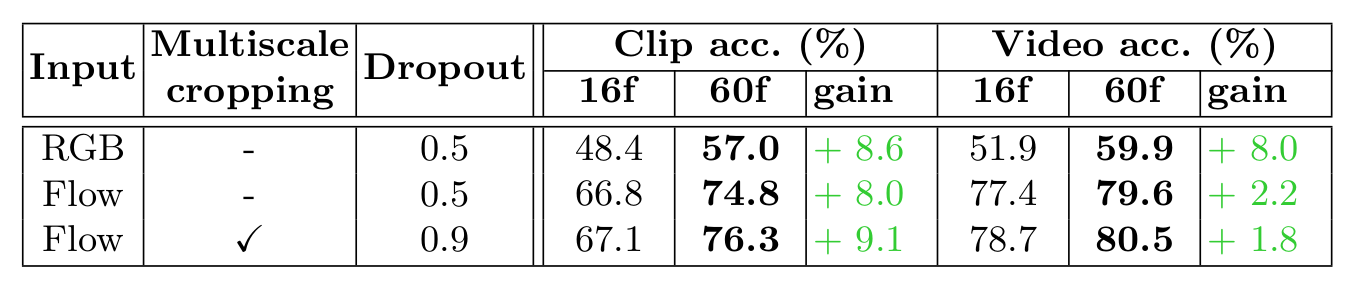
\includegraphics[width=\textwidth]{img_deep/longterm_16vs60}
    \caption{Action recognition accuracy of the two baseline architectures, evaluated on UCF-101 (split1). \textbf{16f} corresponds to the architecture with 16 frame inputs, \textbf{60f} corresponds to 60 frame inputs. \cite{varol_long-term_2016}}
    \label{tab:longterm_16vs60}
\end{table}

The authors note, that the complexity of both networks, i.e.\ the number of trainable parameters, is similar since the 60 frame network processes frames at reduced resolution.

The networks are also evaluated on the HMDB-51 dataset.
Both networks are either trained from scratch, i.e.\ with randomly initialized inputs, or have been pre-trained on UCF-101, which is much bigger than HMDB-51 (see section \ref{chap:datasets}).
Results are shown in table \ref{tab:longterm_pretraining} below.

\begin{table}[H]
    \centering
    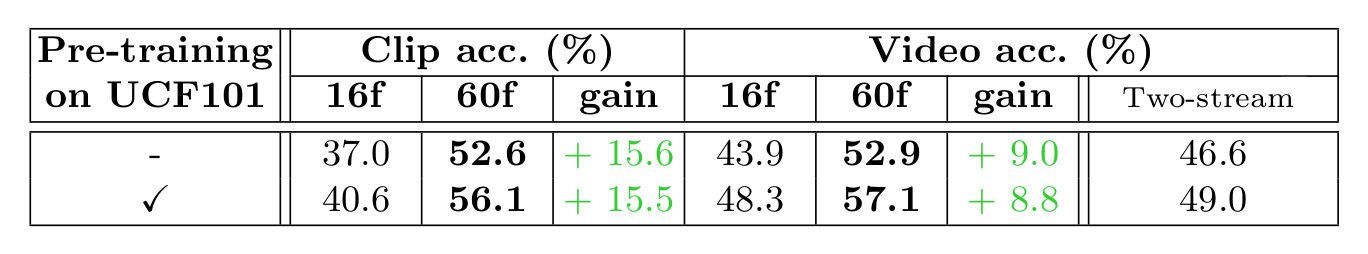
\includegraphics[width=\textwidth]{img_deep/longterm_pretraining}
    \caption{Action recognition accuracy of the two baseline architectures, evaluated on HMDB-51 (split1) with optional pre-training on UCF-101. \textbf{16f} corresponds to the architecture with 16 frame inputs, \textbf{60f} corresponds to 60 frame inputs. \cite{varol_long-term_2016}}
    \label{tab:longterm_pretraining}
\end{table}

The results again indicate, that using long-term temporal convolutions leads to significant increase in action recognition accuracy and that pre-training the networks on a larger dataset yields significant improvement over training it from scratch. 

In order to systematically investigate the influence of temporal extent on action recognition performance, the authors implement their architecture with different numbers of input frames $T = \{20, 40, 60, 80, 100\}$ and different spatial resolutions $\{58 \times 58, 71 \times 71\}$.
Results are shown in the following figure \ref{fig:longterm_systematical}.

\begin{figure}[H]
    \centering
    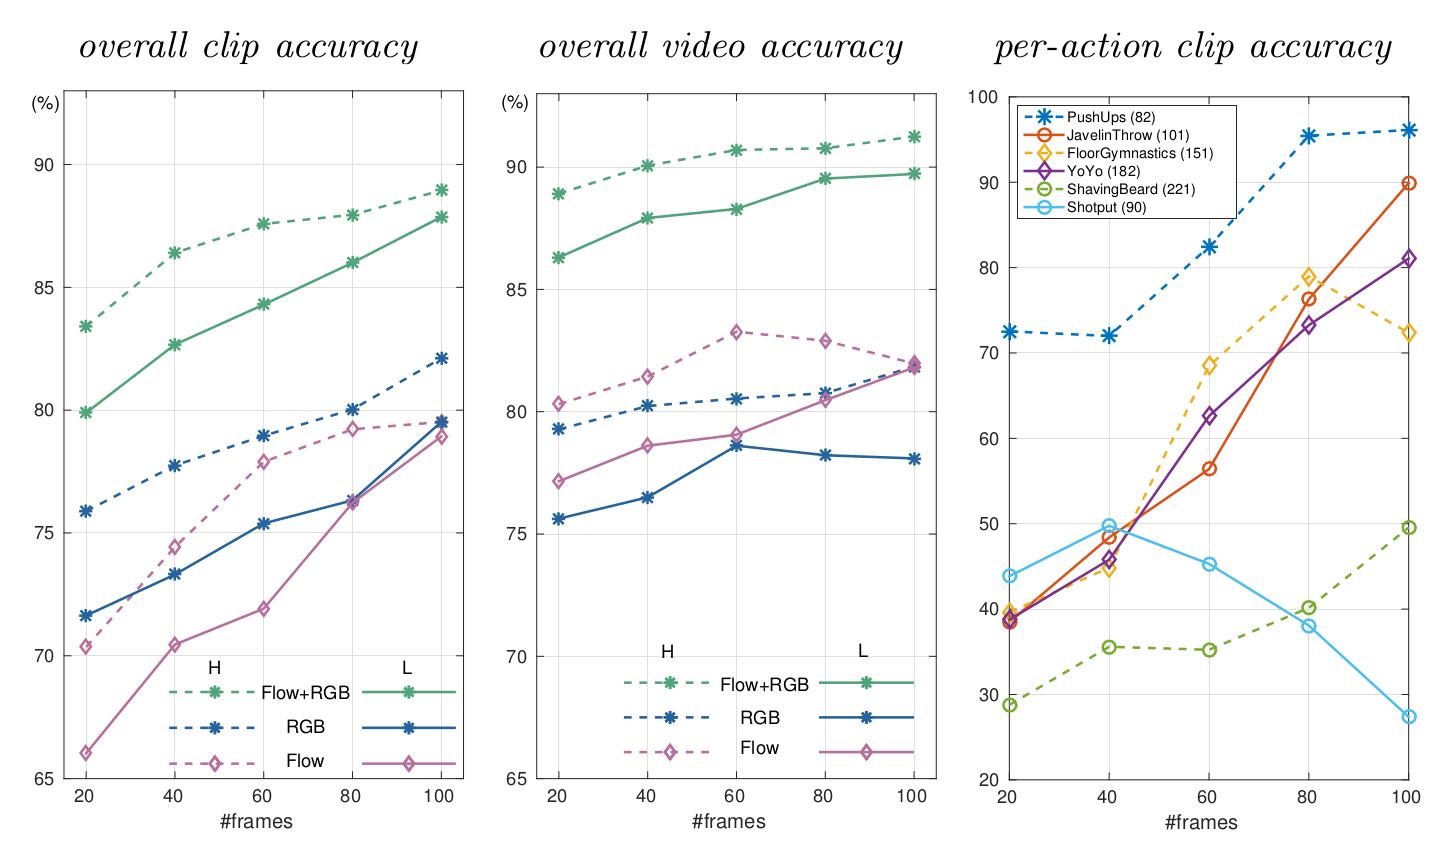
\includegraphics[width=\textwidth]{img_deep/longterm_systematical}
    \caption{Action recognition performance of long-term convolutional networks for varying number of input frames, evaluated on UCF-101 (split1). \textit{H} denotes high resolution ($71 \times 71$ pixel), \textit{L} denotes low resolution ($58 \times 58$ pixel). \cite{varol_long-term_2016}}
    \label{fig:longterm_systematical}
\end{figure}

To conclude, \textcite{varol_long-term_2016} show, that longer temporal extent increases the action recognition accuracy of 3D convolutional neural network for action recognition from video.

%The networks are trained on the UCF-101 and HMDB-51 dataset using stochastic gradient descent with negative log-likelihood criterion.
%
%Details of the testing-procedure are:
%\begin{enumerate}
%    \item The video under test is divided into sequences of length $T$ with temporal stride 4, each called a clip.
%    \item For each video clip, 10 crops are being classified: The 4 corners, the center and their horizontal flips.
%    \item The overall video classification is obtained by averaging over crop scores and clip scores.  
%\end{enumerate}
%
%Two evaluation metrics are used to compare the networks: 
%\begin{enumerate}
%    \item Clip-accuracy: Each clip is assigned the class according to the highest softmax-score and the number of correctly classified clips is measured.
%    \item Video-accuracy (i.e. the standard evaluation protocol): The per-clip softmax scores are averaged and the maximum value defines the class label for the video. The authors report their final resutlts by taking the mean over the results on the three test splits of the datasets.
%\end{enumerate}

%---------------------------------------------------------------------------------------------------------------------------------------------------------------------------------------
\newpage
\subsection{Multiple Stream Networks}


\subsubsection{Two-Stream Convolutional Networks for Action Recognition in Videos (2014)}

\textcite{simonyan_two-stream_2014} propose a novel architecture for action recognition with separate spatial and temporal recognition streams, which are fused late (see figure \ref{fig:twostream_architecture}.
This approach is motivated by the two-streams hypothesis \cite{goodale_separate_1992}, according to which the human visual cortex contains two paths: the ventral stream for object recognition and the dorsal stream for recognising motion.

The authors evaluate two different fusion methods: building the average of both network's outputs and training a linear multi-class SVM on them.
Both streams are implemented as deep CNNs, with rectification activation function for all hidden units.

\begin{figure}[H]
    \centering
    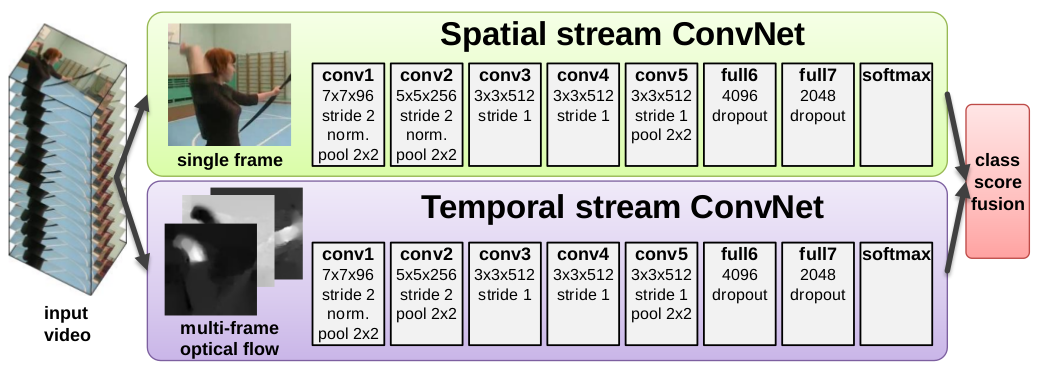
\includegraphics[width=0.9\textwidth]{img_deep/twostream_architecture}
    \caption{Two-stream architecture for video classification \cite{simonyan_two-stream_2014}}
    \label{fig:twostream_architecture}
\end{figure}

The spatial stream takes single video frames as input and is fairly competitive on its own.
Since it is basically an image recognition architecture, it performs action recognition from still video frames.
%This is advantageous, because it can be pre-trained on large image datasets, such as ImageNet \cite{deng_imagenet:_2009}.
The spatial part of a video, i.e. the individual static frames, conveys information about the objects and persons in the scene.

The temporal stream is trained to recognize actions from motion given in the form of optical flow.
The temporal part of a video, i.e. the difference between adjacent static frames, conveys information about the movement of the observer (camera) and the movement of objects in the scene.
The authors propose two methods for constructing the input to the temporal network by stacking optical flow displacement fields along several consecutive frames of the input video.
%The second normalisation layer was removed from the temporal stream network in order to reduce memory usage.

\textbf{Optical Flow Stacking:} \\
A dense optical flow field $\mathbf{d}_t(u,v)$ of two consecutive frames at times $t$ and $t+1$ can be thought of as a two dimensional vector-field, which maps the displacement of each pixel along the transition from frame $t$ to $t+1$.
In this case $u,v \in \mathbb{N}$ correspond to a position in the frame, $1 \leq u \leq w$ and $1 \leq v \leq h$, where $w$ and $h$ are the width and height of the video frames.

The horizontal and vertical components $d_t^x(u,v)$ and $d_t^y(u,v)$ can be interpreted as image channels.

This method constructs the input volume $I_\tau \in \mathbb{R}^{w \times h \times 2L}$ of the temporal stream network by stacking the horizontal and vertical components of the dense optical flow field along $L$ consecutive frames, beginning at time $\tau$. Formally, with $1 \leq k \leq L$:
\begin{align*}
    I_\tau(u,v,2k-1) = d_{\tau + k - 1}^x(u,v) \\
    I_\tau(u,v,2k) = d_{\tau + k - 1}^{y}(u,v)
\end{align*}

\begin{figure}[H]
    \centering
    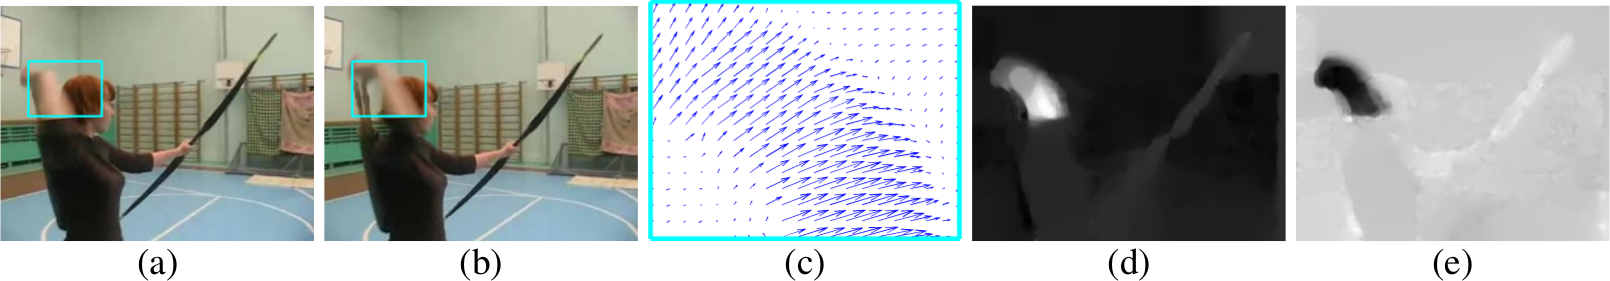
\includegraphics[width=\textwidth]{img_deep/twostream_flow}
    \caption{Optical flow between two frames (a) and (b). (c) shows the dense optical flow field, i.e.\ displacement vectors, of the turquoise region. (d) and (e) illustrate the $x$ and $y$ components of the flow field as images. \cite{simonyan_two-stream_2014}}
    \label{fig:twostream_flow}
\end{figure}

\textbf{Trajectory Stacking:} \\
Instead of sampling at fixed locations in each frame, trajectory stacking samples the dense optical flow field along motion trajectories of the initial points in frame $\tau$.
Let $\mathbf{p}_k$ denote the motion trajectory of initial point $(u,v)$.
With $1 < k \leq L$ and \mbox{$\mathbf{p}_1 = (u,v)$} the trajectory is recursively defined by:

\begin{align*}
    \mathbf{p}_k = \mathbf{p}_{k-1} + \mathbf{d}_{\tau + k - 2}(\mathbf{p}_{k-1})
\end{align*}

The optical flow input volume $I_\tau$ can then be constructed by sampling the horizontal and vertical optical flow components along these trajectories.
Specifically:

\begin{align*}
    I_\tau(u,v,2k-1) = d_{\tau + k - 1}^x(\mathbf{p}_{k}) \\
    I_\tau(u,v,2k) = d_{\tau + k - 1}^y(\mathbf{p}_{k})
\end{align*}

\begin{figure}[H]
    \centering
    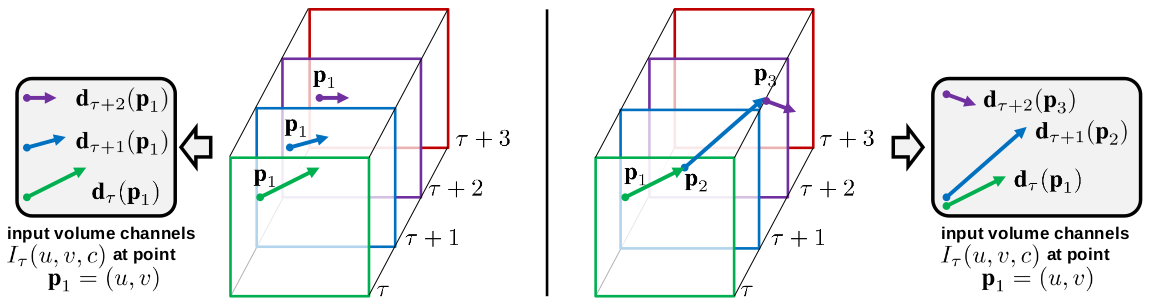
\includegraphics[width=0.9\textwidth]{img_deep/trajectory_stacking}
    \caption{Construction of input volumes from multi-frame optical flow. Left: Optical Flow Stacking. Right: Trajectory Stacking. \cite{simonyan_two-stream_2014}}
    \label{fig:trajectory_stacking}
\end{figure}

The authors further describe two optional techniques that are evaluated for constructing the inputs with either one of optical flow stacking methods.
\begin{enumerate}
    \item \textbf{Bi-directional Optical Flow}: The input volume $I_{\tau}$ is created by using regular forward optical flow from frame $\tau$ to $\tau + L/2$ and additionally calculated optical flow from frame $\tau$ to $\tau - L/2$ in the backwards direction. Stacking the horizontal and vertical components of these optical flow fields results in an input volume of length $L$ around frame $\tau$. 
    \item \textbf{Mean flow subtraction}: The displacement vectors between two frames can dominantly be caused by global movement of the camera. Compared to regular camera-motion compensation, the authors use a simpler approach and just subtract the mean vector from each displacement field $\mathbf{d}_t$.
\end{enumerate}

Since convolutional networks require fixed sized inputs, a $224 \times 224 \times 2L$ subvolume is randomly sampled from $I_\tau \in \mathbb{R}^{w \times h \times 2L}$ and use it as the temporal networks input.
By using optical flow, a representation of motion is explicitly incorporated in the action recognition architecture.

An advantage of separating the spatial and the temporal stream is the possibility of pre-training the spatial stream network with large pre-existing image datasets.
The authors use the dataset of the ImageNet Large Scale Visual Recognition Competition ILSVRC 2012 \cite{russakovsky_imagenet_2015} for pre-training.

The temporal stream network is trained, according to the multi-task learning paradigm \cite{collobert_unified_2008}, on the UCF-101 and the HMDB-51 dataset simultaneously. 
By training a network on several tasks, the network learns more general video representations, since the second task acts as regularizer and more data can be utilized.
This is implemented by using two softmax classification layers, one for each dataset.
Each softmax layer has its own loss function and the sum of the individual losses is taken as the overall training loss for computing the weight updates by backpropagation.

Training for both networks is conducted with mini-batch gradient descent with 256 randomly selected videos at each iteration.
From each of those videos, a single frame is randomly chosen, a $224 \times 224$ sub-image is randomly cropped, randomly horizontal flipped, RGB jittered and then used as training input for the spatial stream network.
An optical flow volume is constructed for this selected frame as described above and used as input for the temporal stream network.

%For optical flow computation the authors use a fast implementation (0.06s per pair of frames) from the OpenCV toolbox.
%Despite it's speed, on-the-fly computation of optical-flow would be a bottleneck and is therefore pre-computed and stored for the complete datasets.

%The creators of UCF-101 and HMDB-51 provide three splits of their datasets into training- and testing-data.
%The standard evaluation procedure is to report the average accuracy over those three splits, which the authors follow in this work as well.

Different setups of the spatial and temporal stream network are evaluated individually on the UCF-101 dataset for creating the final design of the two-stream architecture.
Besides using two different dropout rates ($0.5$ and $0.9$), the performance of the \textbf{spatial}-stream network is evaluated for:
\begin{enumerate}
    \item Training the complete network from scratch on UCF-101.
    \item Pre-training the network on ILSVRC-2012 and fine-tuning it on UCF-101.
    \item Pre-training the network on ILSVRC-2012 and fine-tuning of only the last (classification) layer.
\end{enumerate}

For evaluating the \textbf{temporal}-stream network, a fixed dropout rate of $0.9$ is chosen.
The performance is then measured for:
\begin{enumerate}
    \item Using one or several (stacked) optical flow displacement fields; $L \in {1,5,10}$.
    \item Regular optical flow stacking.
    \item Trajectory stacking.
    \item Using bi-directional optical flow.
    \item Using mean subtraction.
\end{enumerate}

The findings are presented in table \ref{tab:twostream_archeval}.
\begin{table}[H]
    \centering
    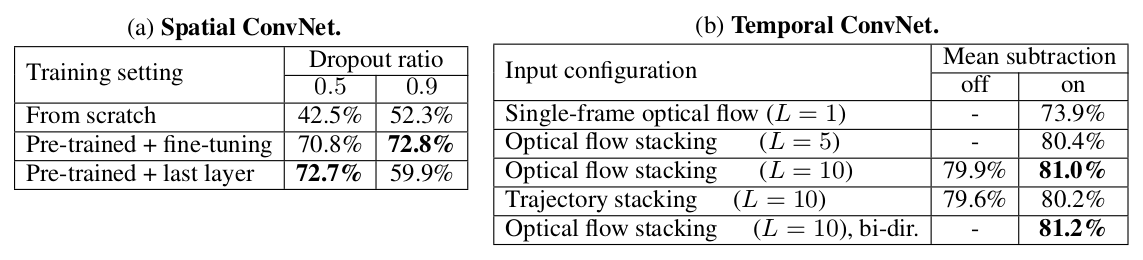
\includegraphics[width=\textwidth]{img_deep/twostream_archeval}
    \caption{Performance of the individual convolutional networks on UCF-101 (split 1) \cite{simonyan_two-stream_2014}}
    \label{tab:twostream_archeval}
\end{table}

Regarding these results, the authors decide on pre-training the spatial-stream network on ILSVRC and fine-tuning only the last layer for the design of the final two-stream architecture.
In the temporal-stream network mean subtraction and stacking multiple optical flow images is beneficial, so $L=10$ is used as the default setting.
Regular optical flow stacking performs better than trajectory stacking and bi-directional optical flow only yields slight improvement against forward optical flow.
Therefore regular forward optical flow stacking is chosen for the temporal-stream network.

The authors highlight that the temporal-stream network significantly outperforms the spatial-stream network, which confirms the importance of motion information for action recognition from video.

After finding the optimal configurations for the individual temporal-stream and spatial-stream networks, different fusion methods (averaging and SVM) are being evaluated.
Fusion by SVM performs best, as can be seen in table \ref{tab:twostream_results}.
The fused network's performance significantly improves over the individual network's performance, which implies, that the spatial and temporal recognition stream are complementary.

\begin{table}[H]
    \centering
    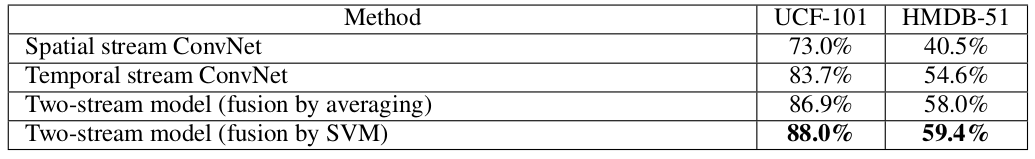
\includegraphics[width=\textwidth]{img_deep/twostream_results}
    \caption{Mean accuracy over the three provided splits of UCF-101 and HMDB-51 \cite{simonyan_two-stream_2014}}
    \label{tab:twostream_results}
\end{table}

The results of \textcite{simonyan_two-stream_2014} show, that their two-stream architecture is a competitive approach in human action recognition from video.


\subsubsection{Beyond Short Snippets: Deep Networks for Video Classification (2015)}

\textcite{ng_beyond_2015} hypothesize that a global video description, that is a representation learned from the full temporal evolution of an input video, is essential for accurate action recognition.
Similar to the approaches of \textcite{baccouche_sequential_2011} and \textcite{varol_long-term_2016}, the goal is to design and evaluate video processing architectures, that are able to incorporate temporal information over long periods in the order tens of seconds, but preferably over the complete video.
In doing so, it is challenging to construct video representations with fixed number of parameters from videos with variable length.

The authors discuss the results of \textcite{karpathy_large-scale_2014}, who discovered that spatio-temporal 3D convolutions applied on frame stacks of short video-subclips only yield marginally better performance than a single-frame baseline.
The following approach therefore does not require 3D convolutions and is illustrated in figure \ref{fig:beyondshort_overview}):

\begin{enumerate}
    \item CNN image features are obtained from the individual frames of an input video with a 2D ConvNet.
    \item The resulting feature vectors, i.e.\ the activations of the ConvNet's last convolutional layer for each frame, are aggregated into a global video representation by one of the following methods:
    \begin{itemize}
        \item The ConvNet is applied to a set of input frames in parallel. Feature pooling layers, which are added after the ConvNets, aggregate their activations into a final video representation.
        \item The ConvNet is applied to a single input frame per time-step. A recurrent neural network (RNN) with layers of LSTM cells \cite{hochreiter_long_1997} is added after the ConvNet to integrate frame information over time.
    \end{itemize}
\end{enumerate}

\begin{figure}[H]
    \centering
    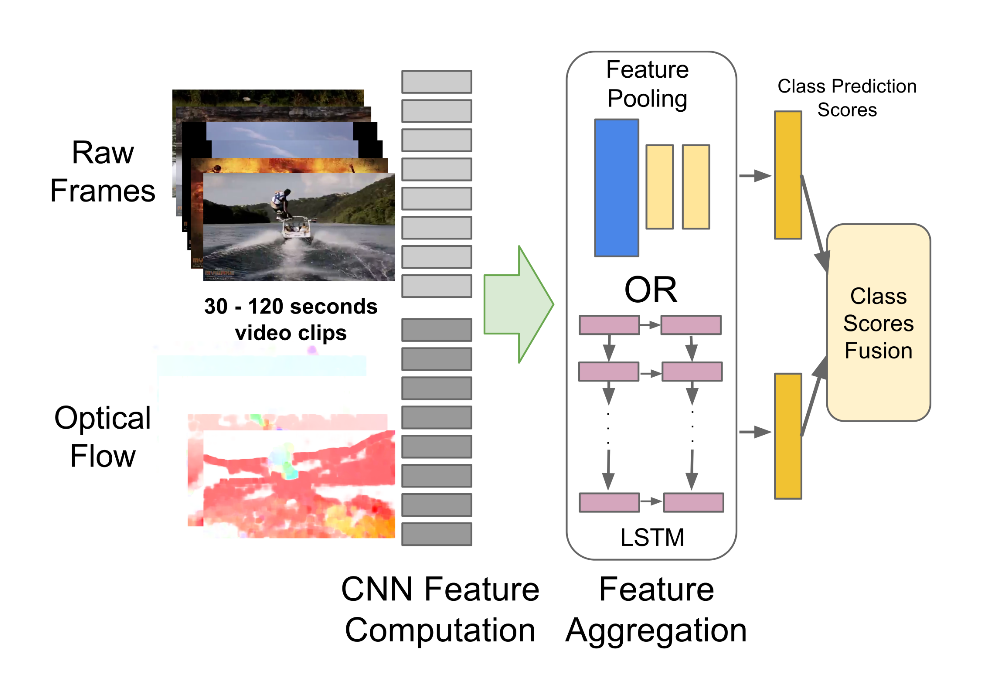
\includegraphics[width=0.8\textwidth]{img_deep/beyondshort_overview}
    \caption{Overview of the approach taken by \textcite{ng_beyond_2015}}
    \label{fig:beyondshort_overview}
\end{figure}

An advantage of this approach is that it can build on the independent achievements of CNN-based image processing architectures by directly embedding them as feature extractors for each frame.
Hence two CNN architectures are being separately evaluated for this task:

\begin{enumerate}
    \item AlexNet \cite{krizhevsky_imagenet_2012}
    \item GoogLeNet \cite{szegedy_going_2015}
\end{enumerate}

Both networks take $220\times220$ pixel sized inputs.
When evaluating the two different architectures without pre-training on frames of the Sports-1M dataset, GoogLeNet consistently outperforms AlexNet.
Nonetheless both architectures are used for the following evaluation.

The temporal extent of this approach can be easily adjusted by changing the number of CNNs that are applied to input frames in parallel before being pooled.
The LSTM models are not limited to a fixed input size and could in general process a complete video in a single pass.
The CNNs, when applied in parallel, all share weights, which results in a constant number of trainable parameters over the number of input frames.

The authors propose to process input videos at only one frame per second, for being able to cover a long temporal extend while remaining computationally feasible.
Therefore implicit motion information from adjacent frames is lost at this framerate.
This is compensated by also using explicit motion information, through optical flow inputs.

\textbf{Feature Pooling}\\
Different configurations of pooling layers are evaluated for combining feature vector representations of individual input frames, as illustrated in figure \ref{fig:beyondshort_poolingarchitectures}.
The authors consider, max-pooling, average pooling as basic pooling operations.
Max-pooling results in faster learning and was therefore chosen as the default pooling method in this approach. 
The pooling architectures additionally include, fully connected layers, time-domain convolution layers and soft-max layers, as described below.

\begin{figure}[H]
    \centering
    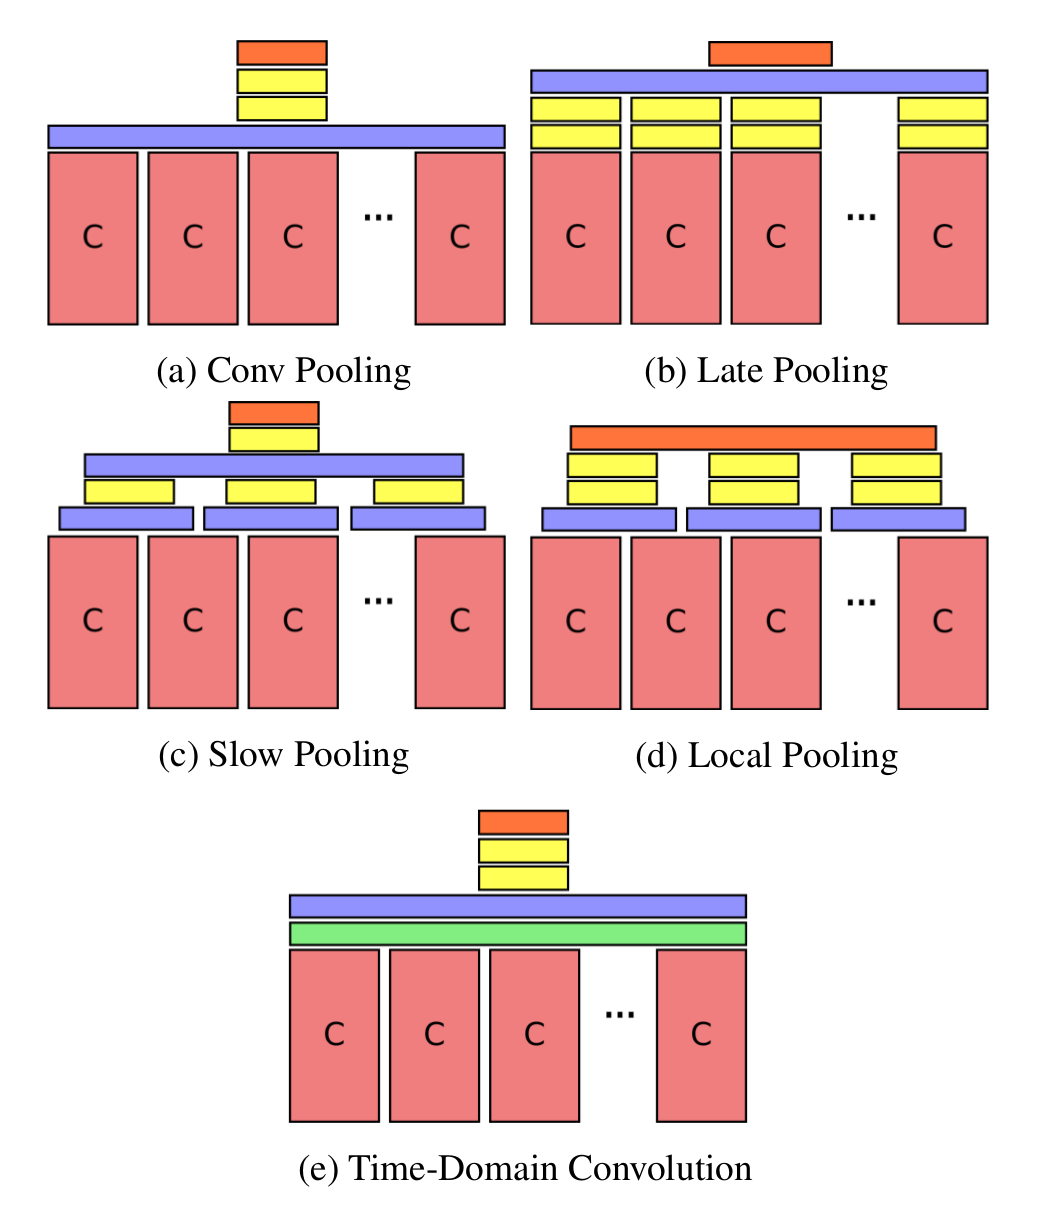
\includegraphics[width=0.6\textwidth]{img_deep/beyondshort_poolingarchitectures}
    \caption{Evaluation of feature pooling architectures with: (Blue) max-pooling layers. (Green) time-domain convolution layers. (Yellow) fully-connected layers. (Orange) soft-max layers. \cite{ng_beyond_2015}}
    \label{fig:beyondshort_poolingarchitectures}
\end{figure}

\begin{enumerate}[label=\alph*)]
\item \textbf{Conv Pooling:} Max-pooling is performed directly over the activations of the final convolutional layers across all input frames, followed by two fully-connected and a soft-max layer.
\item \textbf{Late Pooling:} Convolutional activations are first passed through two fully connected layers individually, before max-pooling is applied over the resulting high-level representations. Weights are shared between all fully-connected layers.
\item \textbf{Slow Pooling:} Two stages of pooling are applied: The first stage combines local temporal patches by max-pooling and feeds the activations into fully connected layers with shared weights. A single max-pooling layer then combines the resulting activations of all fully connected layers in the second stage.
\item \textbf{Local Pooling:} Similar to slow pooling frame information is combined in local temporal patches but only one stage of max-pooling is implemented. This prevents a potential loss of temporal information.
\item \textbf{Time-Domain Convolution:} An additional convolutional layer is implemented before pooling features across frames. It is called \textit{time-domain convolution} since the convolutional layer is applied on features that originate from several frames.
\end{enumerate}

\textbf{LSTM architecture}\\
As an alternative for for capturing dynamic content, i.e.\ the information that is encoded in the differences between frames, a LSTM architecture \cite{hochreiter_long_1997} with 5 layers containing 512 memory cells each is used to aggregate sequences of frame-level CNN activations.
The following figure \ref{fig:beyondshort_lstmarchitecture} shows the approach unfolded in time for 8 timesteps.

\begin{figure}[H]
    \centering
    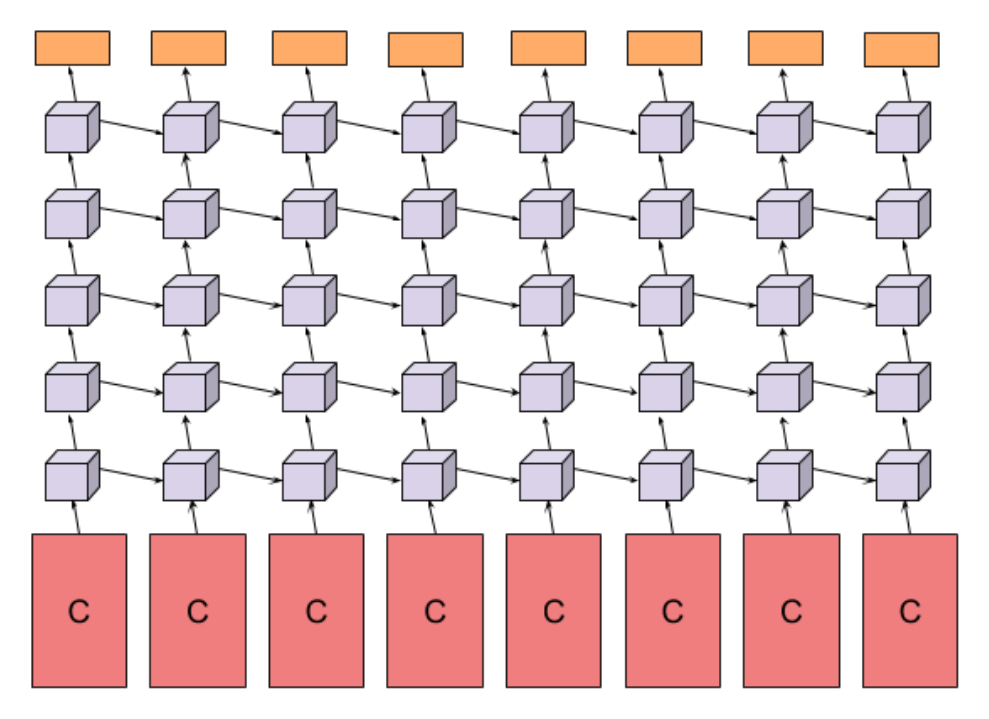
\includegraphics[width=0.6\textwidth]{img_deep/beyondshort_lstmarchitecture}
    \caption{LSTM Architecture. Five layers of LSTM cells process the final CNN activations. The video class is predicted at every timestep by a softmax output layer after the LSTM layers. \cite{ng_beyond_2015}}
    \label{fig:beyondshort_lstmarchitecture}
\end{figure}

In the final architecture, analogously to the two-stream approach of \textcite{simonyan_two-stream_2014}, each of the above described methods is evaluated in a two-stream setup.
The authors train two instances of a model, one on raw video frames, the other on optical flow and perform late fusion over the two resulting streams.
The used optical flow inputs are sampled at 15\textit{fps} by using the method proposed in \cite{zach_duality_2007a}.
Evaluation is performed on the Sports-1M and UCF-101 dataset.

%\textbf{Evaluation}
%The max-pooling architectures were trained on a computing cluster using a distributed version of gradient descent training called \textit{Downpour Stochastic Gradient Descent} \cite{dean_large_2012}.

For training and testing on Sports-1M, the first 5 minutes of each input-video are sampled at 1\textit{fps}, which results in 300 potential input frames per video.
The frames are first resized to $256\times256$ pixel, then a $220\times220$ pixel region of a randomly selected starting frame is selected and the desired number of following frames is cropped accordingly to create an input.
Additionally input frames are flipped horizontally with a probability of 50\%.

Models capable of processing up to 120 frames in a single example are trained, which corresponds to a temporal extent of 2 minutes of video.
To obtain a video-level classification, 240 random input examples are generated from a video for testing as described above and the predictions are averaged.

At first pooling methods are being evaluated with AlexNet CNN and 120 frames as input.
Results show, as given in table \ref{tab:beyondshort_poolingevaluation}, that the conv-pooling architecture yields the best accuracy on Sports-1M dataset.

\begin{table}[H]
    \centering
    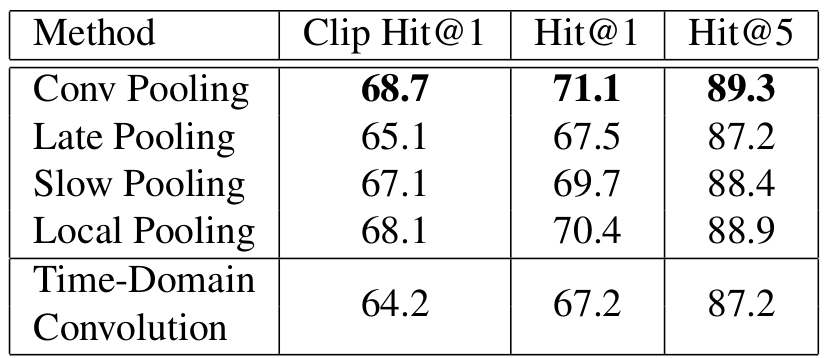
\includegraphics[width=0.5\textwidth]{img_deep/beyondshort_poolingevaluation}
    \caption{Evaluation of different feature pooling methods on Sports-1M dataset with a 120-frame AlexNet model. \cite{ng_beyond_2015}}
    \label{tab:beyondshort_poolingevaluation}
\end{table}

Fine tuning the models is found to be crucial for high performance.
The CNN networks were initialized using pre-trained ImageNet models and then fine-tuned on the Sports-1M dataset in order to decrease training time.
Since the CNN models share weights across input frames, the authors note that training time can also be saved by expanding a individually trained single-frame model to 30-frames and then expanding this 30 frame model to 120 frames, by re-training the pooling layers at each step.


Evaluating the influence of the number of input frames confirmed the authors initial hypothesis, that longer sequences of an input video need to be considered for high accuracy in action recognition.
The LSTM method using 30 frame inputs only performs marginally worse than convolutional pooling with 120 frame inputs.
Results are shown in table \ref{tab:beyondshort_framelengtheval}.

\begin{table}[H]
    \centering
    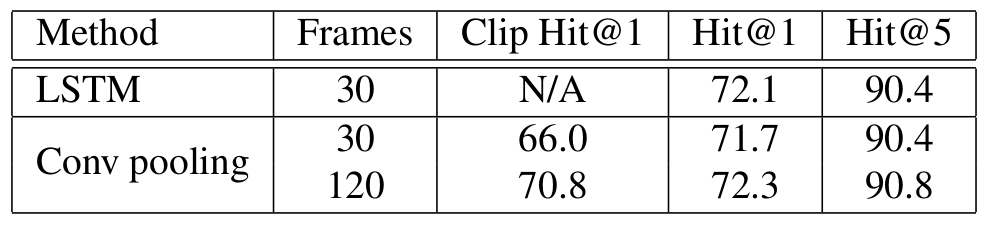
\includegraphics[width=0.6\textwidth]{img_deep/beyondshort_framelengtheval}
    \caption{Comparison of convolutional pooling against LSTM-based RNNs for different numbers of input frames using GoogLeNet CNN models on Sports-1M. \cite{ng_beyond_2015}}
    \label{tab:beyondshort_framelengtheval}
\end{table}

When fusing models with their optical flow counterparts, no significant increase in performance could be observed on the Sports-1M dataset.
Also, the models trained on optical flow evaluated individually yield a much lower performance compared to training on still image frames.
The authors accredit this result to the noisiness of optical flow in the Sports-1M dataset, since it contains real-world videos with low quality and rough cuts.
Overall, the best conv-pooling and lstm models perform significantly better than the state-of-the-art as reported by \textcite{karpathy_large-scale_2014}.

The UCF-101 dataset contains short videos, lasting 10-15 seconds on average.
In comparison to the Sports-1M dataset, optical flow of UCF-101 provides an increase in performance.
The authors best models on UCF-101, which combine image frames and optical-flow, outperform the state of the art reported by \textcite{simonyan_two-stream_2014} by a small margin.


\subsubsection{Towards Good Practices for Very Deep Two-Stream ConvNets (2015)}
\textcite{wang_towards_2015} aim at improving the two-stream ConvNet approach, as introduced by \textcite{simonyan_two-stream_2014}, by leveraging the advances of very deep ConvNet architectures in image classification.
The trends in network design that lead to the success of convolutional architectures in image classification are: smaller convolutional kernels, smaller kernel strides and deeper network architectures.\cite{wang_towards_2015}

Examples of such very deep architectures are GoogLeNet \cite{szegedy_going_2015} and VGGNet \cite{simonyan_very_2014}.
The authors use these two models to create and evaluate enhanced two-stream ConvNet models for video action recognition.

Two main draw-backs of recent ConvNet approaches in video action recognition are identified:
\begin{enumerate}
    \item The applied models are shallow compared to their image counterparts. The deepest variant VGG-19\cite{simonyan_very_2014} contains 16 convolutional layers, while the networks in the original two-stream ConvNet approach contain 5 convolutional layers.
    \item The available dataset are too small, which results in over-fitting.
\end{enumerate}

Considering these deficits, \textcite{wang_towards_2015} therefore propose a set of good practices to enable very deep ConvNet architectures for accurate action recognition, specifically in the two-stream ConvNet architecture.
These namely are:

\begin{enumerate}
    \item Pre-training for the spatial- as well as the temporal-stream network.
    \item Smaller learning rates.
    \item Different and more data augmentation techniques.
    \item Higher drop-out ratios.
\end{enumerate}

The authors apply these good practices to a two-stream approach, which they call \textit{Very Deep Two-Stream ConvNets}.
The spatial net therein processes a single video frame of input size ($224 \times 224 \times 3$) at a time.
It is therefore an image classification architecture and either GoogLeNet or VGGNet is used.

The temporal net processes 10 stacked optical flow inputs, each splitted into images of the $x$- and $y$- coordinate.
Its input therefore has a size of $224 \times 224 \times 20$.
The convolutional kernels in the first layer need to be different than in the spatial stream to process these higher-dimensional inputs.

Evaluation is done using the UCF-101 dataset, specifically on the three splits into training- and test-set, that are provided with it.
For each split, the training set consists of around $10.000$ videos while the test-set consists of $3.000$ videos (further described in section \ref{chap:datasets}).
UCF101 contains 13.320 videos in total and is considered extremely small for training very deep architectures \cite{wang_towards_2015}.

\textbf{Pre-training}\\
The spatial net is pre-trained using an ImageNet model as in \cite{simonyan_two-stream_2014}.
This specifically means, that the network's weights are initialized with the values of a trained ImageNet model.
Interestingly, the authors find that pre-training is also beneficial for the temporal-stream network.
The authors average the ImageNet model's filters across channels and duplicate them 20 times as filters for the temporal net's first layer.

\textbf{Smaller Learning Rates}\\
Since the networks in both streams have been pre-trained, the authors use smaller learning rates as in the original two-stream approach \cite{simonyan_two-stream_2014}.
The authors note a faster conversion of the training and credit this to the pre-training.

\textbf{Data Augmentation Techniques}\\
Data augmentation techniques such as random cropping of inputs and horizontal flipping have been widely used to reduce over-fitting.
Since random cropping favors cropping regions in the center of an image/frame, a corner cropping strategy is proposed.
Specifically this means cropping the four corners and the center of the input images as inputs.
This increases the variation of inputs and reduces over-fitting.

Additionally, network inputs are cropped from video frames on multiple scales.
The input video is first scaled to $256 \times 340$ pixels and the cropping width and height is randomly chosen from $\{256, 224, 192, 168\}$.
The cropped region is then scaled to $224 \times 224$ to form the network input.

\textbf{High Dropout Ratio}\\
The authors use dropout ratios of 0.8 and 0.9 for the fully connected layers at the end of the networks.

The proposed good practices are validates, by training very deep two-stream ConvNet models on the UCF-101 dataset.
For testing, 25 frames or optical flow inputs are sampled from a test video.
For each of these input samples 10 inputs for the very deep ConvNet are created by applying the above mentioned cropping method (four corners, the center and their horizontal flip).
The final prediction is obtained by averaging over all inputs.

The temporal and spatial net are fused, using a weighted linear combination of both outputs.
The weight for the temporal net is set to $2$ and the weight for the spatial net is set to $1$.
Optical flow fields are extracted using the OpenCV implementation of TVL1 optical flow algorithm \cite{zach_duality_2007}.

Table \ref{tab:towardsgood_results} shows the accuracy of the very deep Two-Stream ConvNets.

\begin{table}[H]
    \centering
    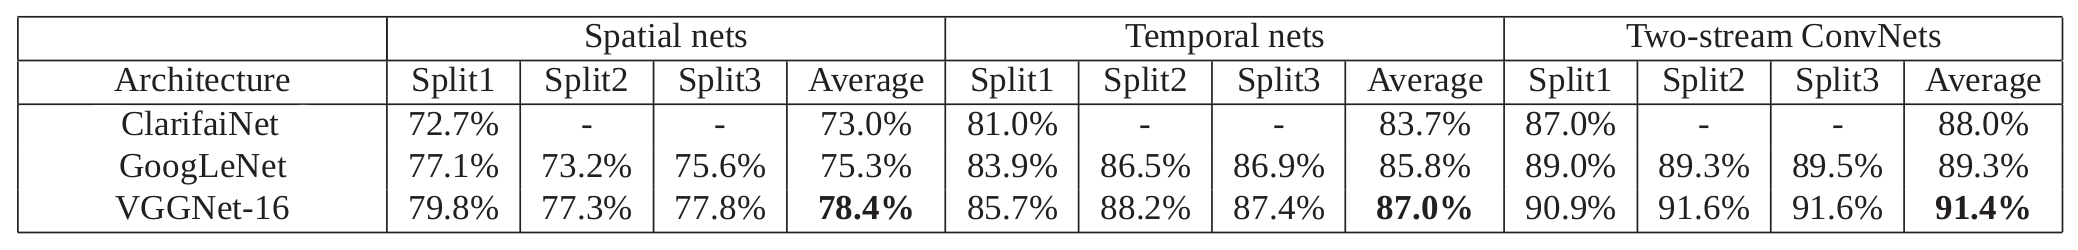
\includegraphics[width=\textwidth]{img_deep/towardsgood_results}
    \caption{Accuracy of the very deep two-stream ConvNet architecture on UCF-101 dataset for different ConvNet models. ClarifaiNet denotes the original two-stream approach and its results are taken from \cite{simonyan_two-stream_2014}. \cite{wang_towards_2015}}
    \label{tab:towardsgood_results}
\end{table}

These results show, that the proposed good practices and using very deep convolutional network models lead to a significant improvement in performance over the original two-stream approach.


\subsubsection{Convolutional Two-Stream Network Fusion for Video Action Recognition (2016)}
\textcite{feichtenhofer_convolutional_2016} identify two deficits of the two-stream architecture\cite{simonyan_two-stream_2014} regarding the fusion of both streams and the processed temporal extent of the temporal stream:
\begin{enumerate}
    \item The architecture is not able to learn pixel-wise relations between the spatial and the temporal stream, i.e.\ it cannot relate extracted object-features to corresponding motion features, since the two separate streams are fused late (at the final softmax-layer).
    \item A temporal extent of only $L = 10$ frames is processed by the temporal stream network in a single pass. In the original approach, this was addressed by averaging network outputs over equally spaced temporal locations in the input video. However this averaging does not consider the temporal evolution of actions.
\end{enumerate}

The authors address these deficits by evaluating fusion methods for better combining the appearance information in the spatial stream network with the motion information in the temporal stream network.
Fusion methods are operations, that combine two feature maps from different ConvNets into a single feature map.
When combining all feature maps in a specific layer of a first network with all the feature maps in a specific layer of another network, the two network streams are fused into one.

Fusion can be conducted either spatially or temporally.
Spatial fusion combines feature maps between the streams of the two-stream architecture, which process information from the same point in time.
Temporal fusion combines feature maps resulting from applying the two-stream architecture to different points in time.

In the original two-stream approach \cite{simonyan_two-stream_2014} both streams are fused spatially by averaging softmax scores of both streams, which is called \textit{late fusion}.
The two-stream network is applied to several randomly sampled temporal locations of an input video and the output scores are temporally fused by averaging.

A fusion function $f: x^a, x^b \rightarrow y$ combines two feature maps $x^a, x^b \in \mathbb{R}^{W \times H \times D}$ into a fused feature map $y \in \mathbb{R}^{W \times H \times D'}$.
$W$ and $H$ correspond to the spatial dimensions of the input frames, which get successively reduced by propagation through the layers.
$D$ and $D'$ correspond to the number of channels, i.e.\ the number of filters in the convolutional layer. 

The following \textbf{spatial fusion} methods are evaluated:

\textbf{Sum Fusion}:\\
Both feature maps are summed element-wise.
The output feature map has the same dimensions as the input feature map.
Since the ordering of the channels is arbitrary in each network stream, this fusion technique does not implement a semantic relation between feature maps.

\textbf{Max Fusion}:\\
This method is similar to Sum Fusion, but the maximum value at each location of the two feature maps is used as the new feature map.
The output feature map has again the same dimensions as the input feature maps and does not represent a semantic relation between the feature maps.

\textbf{Concatenation Fusion}:\\
The two feature maps are stacked into each other along the dimension of channels.
The resulting feature map has dimension $W \times H \times 2D$.
Since the activations are not combined by a mathematical operation, a relation between the feature maps is not implemented but it can be learned by the following layers.

\textbf{Conv Fusion}:\\
The feature maps are first concatenated as described above.
A set of $D$ trainable filters with dimensions $1 \times 1 \times 2D$ is then convolved with the stacked feature maps and a bias is added to produce a resulting feature map of dimension $H \times W \times D$.
The convolution can be seen as a trainable weighted combination of the feature maps across the channels, which is able to learn semantic relations between two feature maps.

\textbf{Bilinear Fusion}:\\
The channel vectors of the feature maps at each pixel locations are combined by computing their matrix outer product.
This results in $H \cdot W$ matrices for each pixel location which are then added to form the new feature map of dimension $D \times D$.
This fusion method is adapted from the Bilinear CNN approach in image classification \cite{lin_bilinear_2015}.
Usually the fully connected layers are replaced by a linear SVM to make this fusion method usable in practice, i.e.\ the compensate the high number of parameters.

Implementing a spatial fusion layer between two network streams has significant influence on the number of trainable parameters in the network, especially if the networks are fused before the fully connected layers and if only the merged stream is kept, since most parameters are located in the fully connected layers.

In figure \ref{fig:streamfusion_layerplacement} two examples of placing fusion layers into the two-stream architecture are illustrated.

\begin{figure}[H]
    \centering
    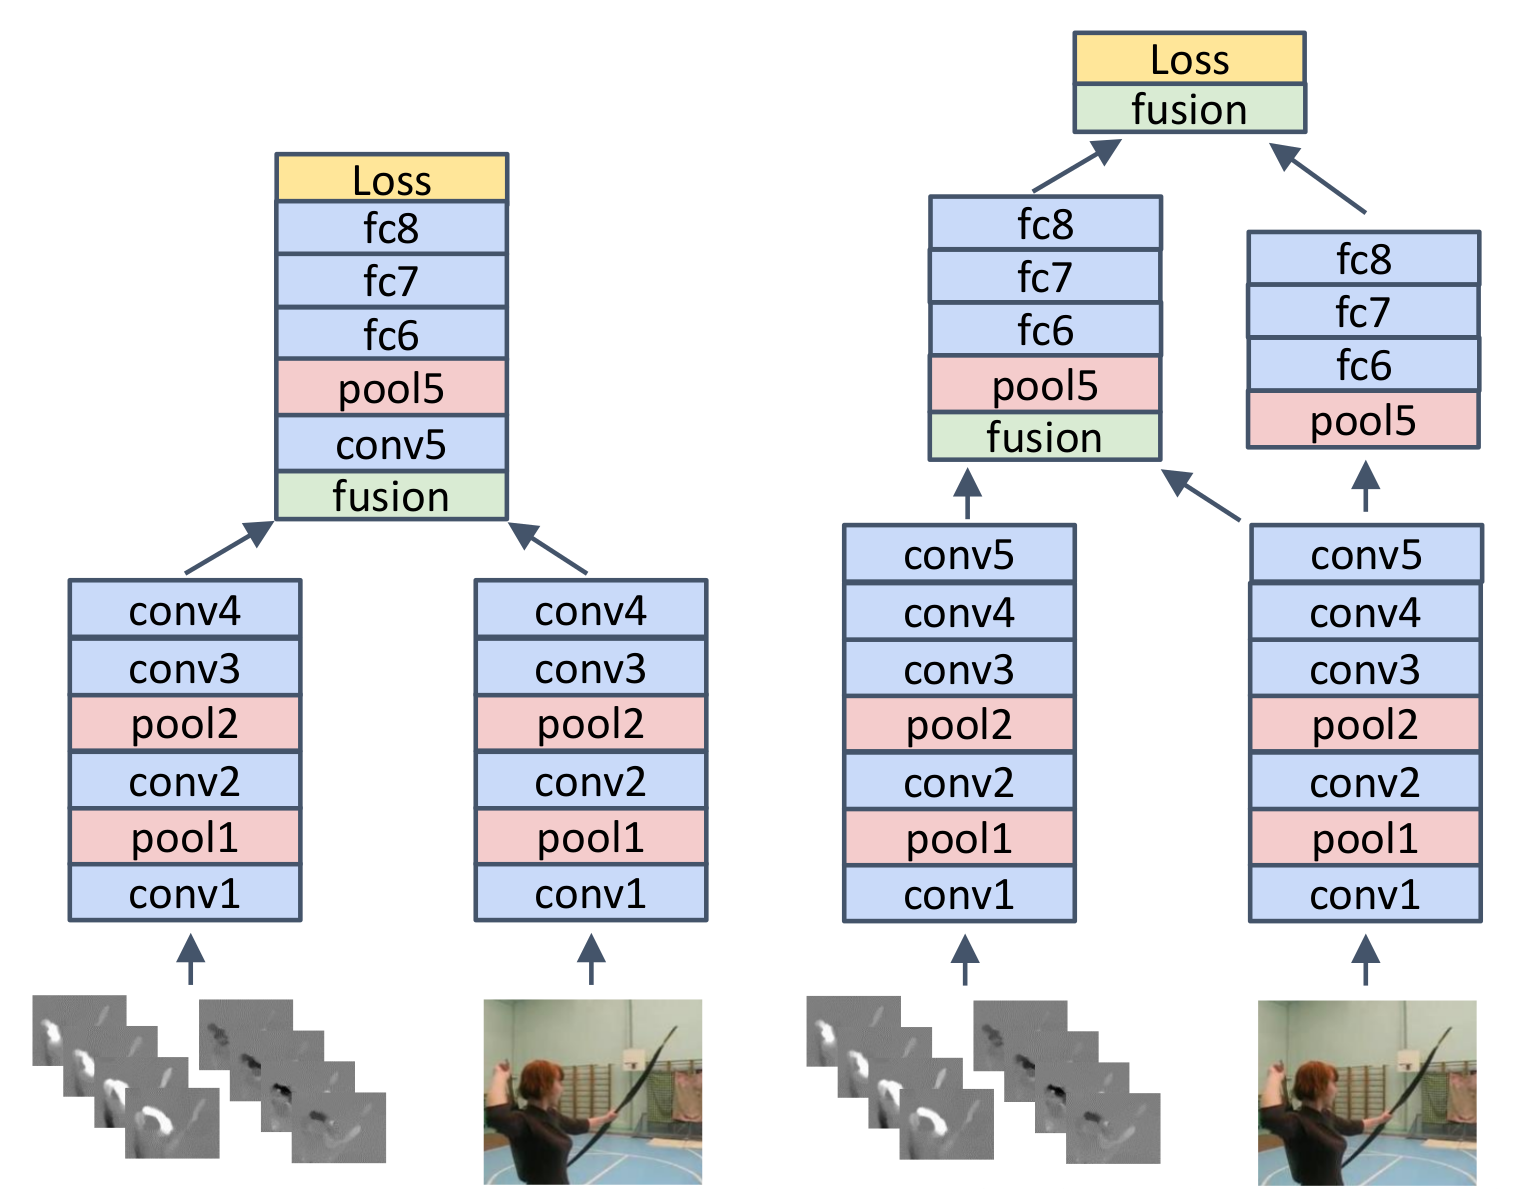
\includegraphics[width=0.75\textwidth]{img_deep/streamfusion_layerplacement}
    \caption{Placement of fusion layers between the spatial and temporal stream in a two-stream architecture. (\textit{left}) Only the merged stream is kept. (\textit{right}) The spatial stream is maintained after first fusion operation and merged before the final layer. \cite{feichtenhofer_convolutional_2016}}
    \label{fig:streamfusion_layerplacement}
\end{figure}

The authors evaluate spatial fusion methods in a two-stream architecture as implemented in the original approach \cite{simonyan_two-stream_2014}.
Each stream consists of 5 convolutional layers, and three fully connected layers.
The accuracy on UCF101 (Split1), the number of parameters and overall number of layers in the architecture is given in table \ref{tab:streamfusion_parameternumber}.
The streams are fused after fifth convolutional layer and only the fused stream is kept.

\begin{table}[H]
    \centering
    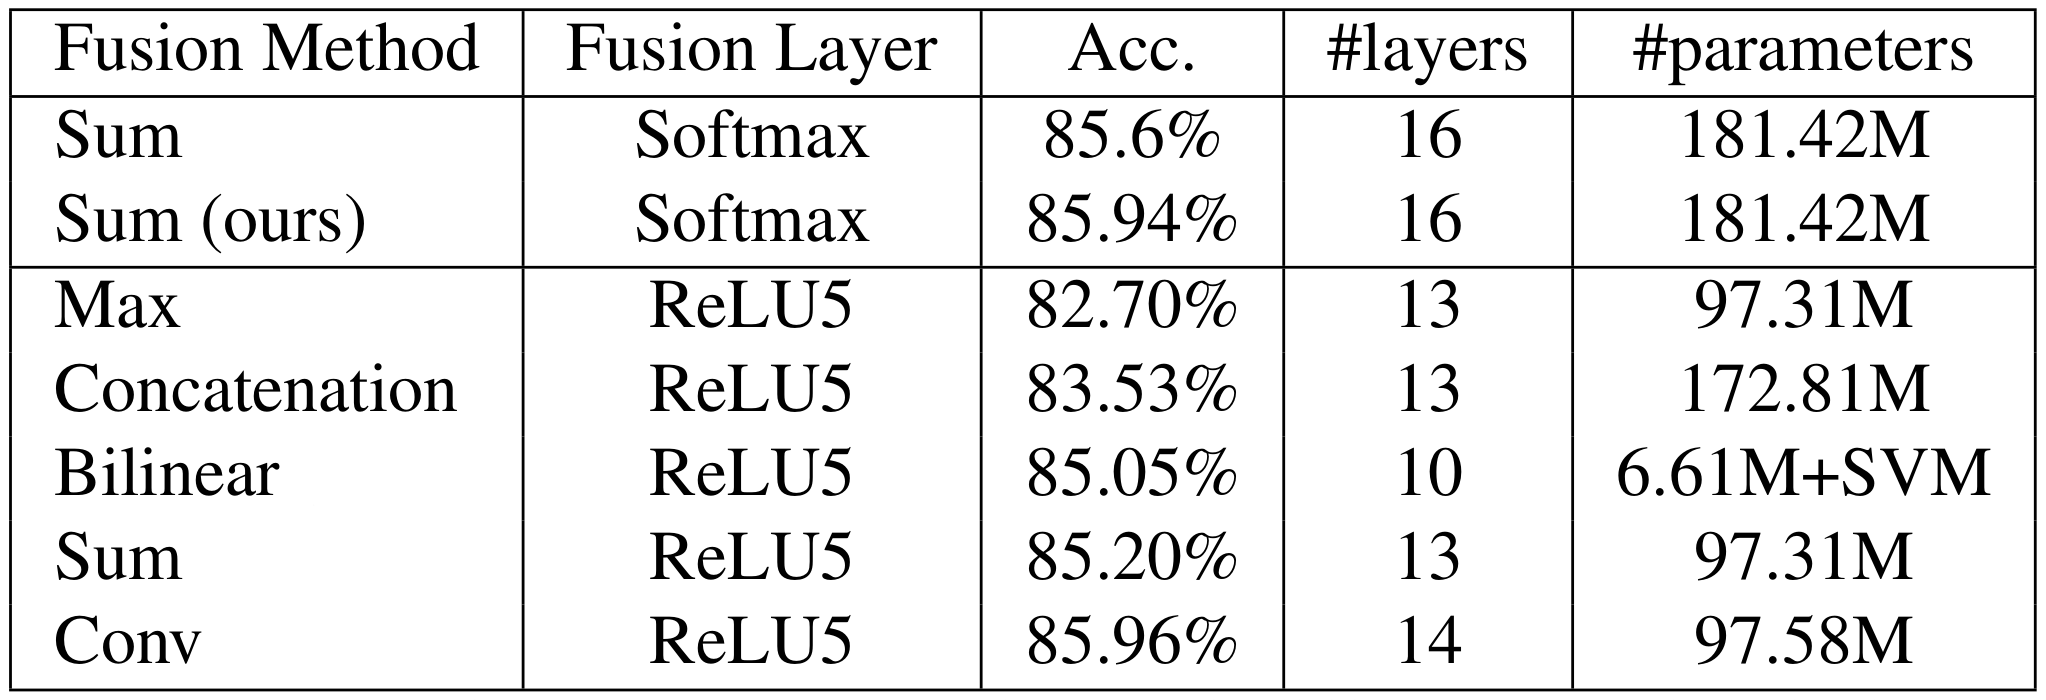
\includegraphics[width=0.7\textwidth]{img_deep/streamfusion_parameternumber}
    \caption{Performance and number of parameters for different spatial fusion methods in a two-stream setup, evaluated on UCF101 (split 1) \cite{feichtenhofer_convolutional_2016}}
    \label{tab:streamfusion_parameternumber}
\end{table}

Results of the original approach are reported in the first row of table \ref{tab:streamfusion_parameternumber}.
The authors' approach yields comparable results, when implementing the same fusion method.
Conv Fusion performs best and reduces the number of parameters significantly to roughly half of the parameters in the original approach.

Implementing the fusion layer after an earlier convolutional layer was found to decreases the performance significantly.
Best results are obtained by fusion after the rectification layer of convolutional layer 5, keeping both streams and fusing again at the final layer (as shown in figure \ref{fig:streamfusion_layerplacement} (right)).

When several inputs from different temporal points in the video are processed in succession, feature maps can be interpreted as being extended over time by stacking them for each input.
In order to fuse information over several inputs, temporal pooling layers can be implemented.
The input to a temporal pooling layer is a feature map $x \in \mathbb{R}^{H \times W \times T \times D}$ where $H$ and $W$ correspond to the spatial dimension, $T$ corresponds to the temporal dimension and $D$ corresponds to the number of channels in the feature map.

The temporal pooling methods shown in figure \ref{fig:streamfusion_temppooling} are evaluated.

\begin{figure}[H]
    \centering
    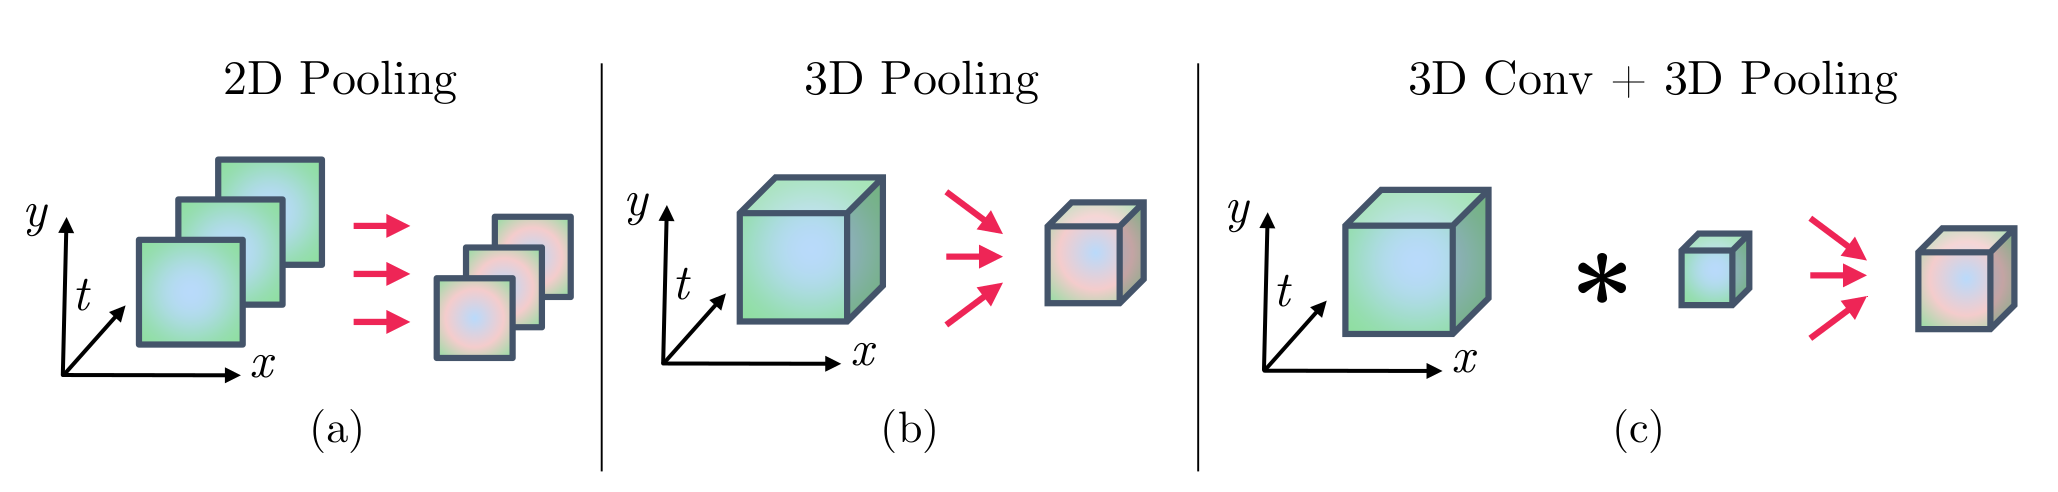
\includegraphics[width=\textwidth]{img_deep/streamfusion_temppooling}
\caption{Methods for pooling feature maps along the temporal dimension. \cite{feichtenhofer_convolutional_2016}}
    \label{fig:streamfusion_temppooling}
\end{figure}

\textbf{a) 2D pooling.}
The feature maps in each channel are only pooled spatially.
The network predictions are averaged over all outputs for different points in time, where the network has been applied.
The pooling operation ignores the temporal dimension.

\textbf{b) 3D pooling.}
Max-pooling with a 3D pooling filter of dimensions $W' \times H' \times T'$ is applied to the stacked feature maps.
The max-pooling operation executed for each of the channels $D$ individually.
Pooling across different channels is not conducted.

\textbf{c) 3D Conv + 3D Pooling.}
A set of $D'$ filters $f \in \mathbb{R}^{W'' \times H'' \times T'' \times D \times D'}$ is convolved with the stacked feature maps and biases are added.
The resulting feature map is then pooled with a 3D pooling filter as described above.
Since the convolutional filter is trainable, it is able to learn weighted combinations of features in a local spatio-temporal region.

Implementing these temporal pooling methods shows, that 3D Conv + 3D Pooling performs best.

Using these previous results, a two-stream convolutional neural network model for action recognition is proposed by the authors as follows:
\begin{itemize}
    \item Two VGG-16 models \cite{simonyan_very_2014} are used as spatial and temporal stream network (13 convolutional and 3 fully connected layers each).
    \item The temporal stream operates on 10 stacked frames of optical flow and is fused at the last convolutional layer and after the fully connected layers (as illustrated in figure \ref{fig:streamfusion_layerplacement} \textit{right}).
    \item The two-stream model is applied at 5 temporal points in the video with fixed temporal distance.
\end{itemize}

The approach achieves $92.5\%$ accuracy on UCF-101 and $65.4\%$ accuracy on HMDB-51.


\subsection{Pooling of Deeply Learned Features}

\subsubsection{Action recognition with trajectory-pooled deep-convolutional descriptors (2015)}
\textcite{wang_action_2015} propose a novel method for building video representations by combining the advantageous properties of hand-crafted features as in \textit{Dense Trajectories} \cite{wang_action_2013} with deeply learned features as in \textit{Two-Stream Convolutional Networks} \cite{simonyan_two-stream_2014}.

In the \textit{Improved Dense Trajectories} approach \cite{wang_action_2013}, local features are extracted along trajectories, which are mostly located near regions of prominent motion in a video.
\textcite{wang_action_2015} claim however, that hand-crafted features are not discriminative enough for accurate action recognition.

Deep architectures have proven to learn discriminative features effectively with \textit{Two-Stream Networks} being a successful approach that finally performed comparably to \textit{Improved Dense Trajectories}.

The main outline of an approach for combining these two approaches in action recognition is given by the authors as follows:
\begin{enumerate}
    \item A two-stream convolutional network architecture is trained on multiple scales of a large dataset.
    \item \textit{Dense Trajectories} are being extracted from input videos according to the approach in \cite{wang_action_2013}.  
    \item The learned feature maps of the two-stream architecture are used as local feature extractors by pooling the convolutional activations over areas around the trajectories. The resulting descriptor is called trajectory-pooled deep-convolutional descriptor (TDD).
    \item The local TDDs are aggregated over the complete video using the Fisher Vector representation. \cite{sanchez_image_2013}
    \item A linear SVM is trained to assign action labels to the FV representations, i.e.\ to perform action recognition.
\end{enumerate}

%Results show, that TDD is complementary to HOG, HOF and MBH and therefore fusion of these descriptors can further boost performance.

%The authors evaluate their approach on the HMDB51 and UCF-101 dataset.

%In contrast to \cite{wang_action_2013}, trajectories are only extracted on the original spatial scale, because it is computationally more effective.
%To compensate, multi-scale TDDs are extracted around the trajectories.
Any convolutional architecture can be embedded in a two-stream setup for TDD extraction.
The authors choose the Clarifai network \cite{zeiler_visualizing_2014-1} with less filters in the \textit{conv4} layer (512 instead of 1024) and a lower dimensional \textit{full7} layer (2048 instead of 4096).
This architecture is used for implementing the spatial stream network as well as the temporal stream network.
Details are illustrated in table \ref{tab:tdd_layers}) below.

\begin{table}[H]
    \centering
    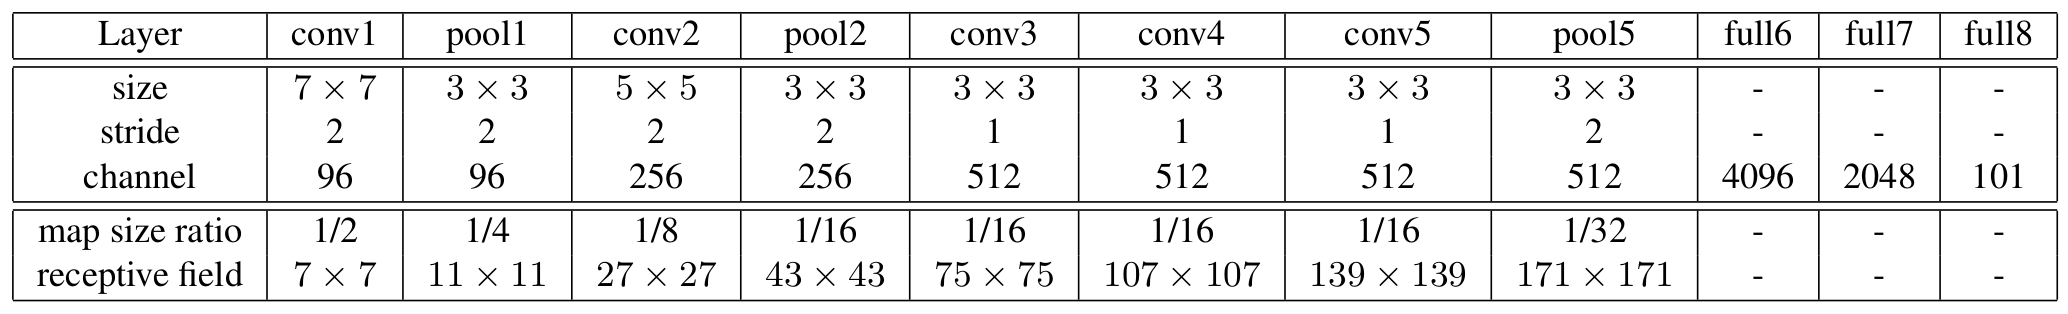
\includegraphics[width=\textwidth]{img_deep/tdd_layers}
    \caption{Layers of the Clarifai network modified for TDD extraction \cite{wang_action_2015}}
    \label{tab:tdd_layers}
\end{table}

%After training the two-stream architecture, the activations of convolutional layers in each stream, i.e.\ the feature maps, are used for extracting the TDD descriptors of an input video.

For each convolutional or pooling layer with kernel size $k$, zero padding of the layer's input is applied with size $\lfloor k/2 \rfloor$.
This padding prevents an additional reduction in dimensionality between the layer's input and output besides the reduction that stems from applying the kernel with a certain stride.
Therefore the position of a trajectory point in the input can be easily related to coordinates in the convolutional feature map at question by incorporating the map size ratio $r$ of the layer, as given in table \ref{tab:tdd_layers}.
Specifically, the $p$-th point in a video trajectory $(x_p, y_p, z_p)$ is represented by point $(\overline{r \cdot x_p}, \overline{r \cdot y_p}, z_p)$.
Where $\overline{(\cdot)}$ denotes the rounding operation.

Given a video $V$, training the two-stream architecture results in a set of feature maps $\mathbb{C}(V)$ from the spatial stream $s$ and temporal stream $t$.
\begin{equation*}
    \mathbb{C}(V) = \{C_1^s, C_2^s, \cdots, C_M^s, C_1^t, C_2^t, \cdots, C_M^t\}
\end{equation*}
where:
\begin{itemize}
    \item $C_m^s, C_m^t \in \mathbb{R}^{H_m \times W_m \times L \times N_m}$ denotes the $m$-th feature map of the spatial or temporal stream
    \item $H_m$ is it's height
    \item $W_m$ is it's width
    \item $L$ is the number of video frames
    \item $N_m$ is the number of channels
    \item $M$ is the number of feature maps in each stream.
\end{itemize}

There are two steps involved in extracting the local trajectory-aligned descriptors (TDD) from a 3D volume around a trajectory:
\begin{enumerate}
    \item Feature Map Normalization (two different methods)
        \begin{itemize}
            \item Spatiotemporal Normalization
            \item Channel Normalization
        \end{itemize}
    \item Trajectory Pooling
\end{enumerate}

\textbf{Feature Map Normalization}\\
Normalization has been widely applied to hand-crafted features because it reduces the influence of illumination.
The authors use this technique on convolutional feature maps to suppress the activation burstiness of some neurons.

In \textit{Spatiotemporal Normalization}, each feature map is normalized independently across each channel according to it's maximal value.
Specifically, for any channel $n$ and a feature map $C \in \mathbb{C}(V)$:
\begin{equation*}
    \tilde{C}_{st}(x,y,z,n) = C(x,y,z,n) / \max_{x,y,z} C(x,y,z,n)
\end{equation*}
Spatiotemporal Normalization ensures, that the feature maps across all channels range in the interval $(0,1)$.

In \textit{Channel Normalization} the values of each feature map are normalized according to the values at the same spatial positions but in another channel.
Specifically, for an spatial position $(x,y,z)$ in the feature map at question:
\begin{equation*}
    \tilde{C}_{ch}(x,y,z,n) = C(x,y,z,n) / \max_{n} C(x,y,z,n)
\end{equation*}
Channel Normalization ensures, that the feature map values of each pixel range in the interval $(0,1)$ and therefore contribute equally to the final representation.

Both normalization methods were evaluated experimentally and the authors found, that combining the resulting video representations from both normalization methods by late fusion yields the best results.

\textbf{Trajectory Pooling}
Given the $k$-th trajectory out of all trajectories $\mathbb{T}(V)$ over a video $V$, a trajectory-pooled deep convolutional descriptor in respect to a normalized feature map $\tilde{C}_m$ is constructed by sum-pooling the feature map values along the trajectory-points in the feature map.

\begin{equation*}
    D(T_k, \tilde{C}_m) = \sum_{p=1}^P \tilde{C}(\overline{(r_m \cdot x_p^k)}, \overline{(r_m \cdot y_p^k)}, z_p^k)
\end{equation*}
Where $r_m$ is the map size ratio belonging to feature map $\tilde{C}_m$.

The extracted TDDs over a complete video are then aggregated using the Fisher Vector representation \cite{sanchez_image_2013} to form a global video representation.
A linear SVM is then trained to learn the action classes to these representations.

\begin{figure}[H]
    \centering
    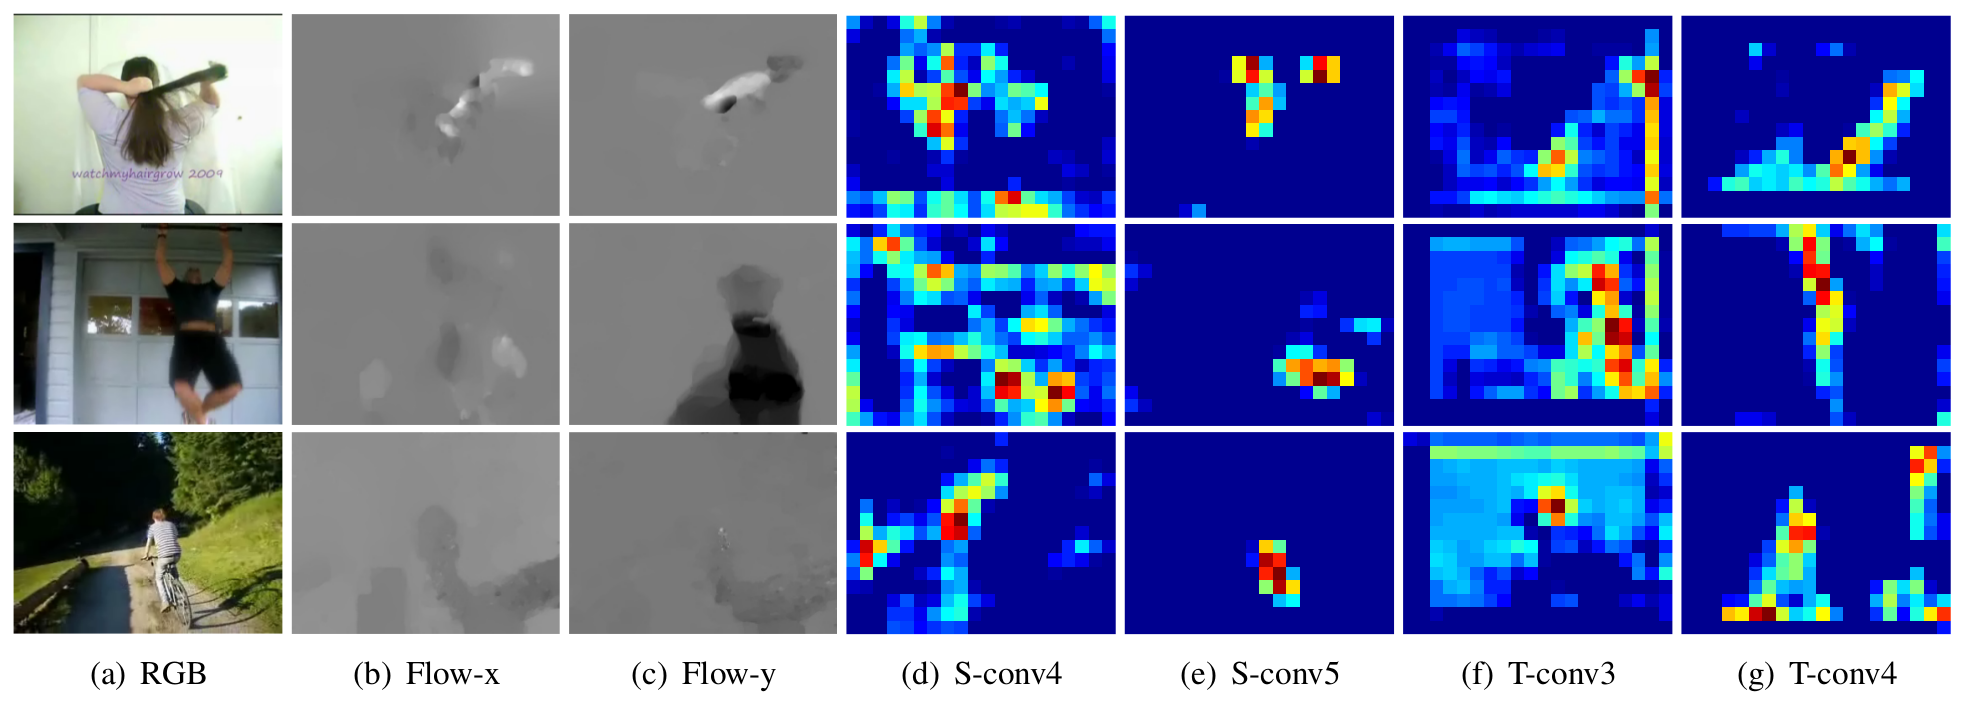
\includegraphics[width=\textwidth]{img_deep/tdd_featuremaps}
    \caption{\textit{a}) Snapshots of input videos. \textit{b-c}) Their corresponding optical flow fields in $x$ and $y$ dimension. \textit{d-g}) The corresponding activations of the feature maps used for TDD extraction \cite{wang_action_2015}}
    \label{fig:tdd_featuremaps}
\end{figure}

Using TDDs for action recognition is evaluated on the UCF-101 and HMDB-51 dataset.
Since UCF-101 is bigger than HMDB-51, the authors initially train the two-stream model on the bigger UCF-101 dataset and transfer it for TDD extraction on HMDB-51.

The weights of the \textbf{spatial net} are initialized using the publicly available model of \cite{chatfield_return_2014} and then fine-tuned on the frames of UCF-101 videos.
During fine-tuning, the frames of UCF-101 are first resized to have 256 pixels on their smallest side.
A randomly cropped region of $224 \times 224$ pixels then builds the network training input after random horizontal flipping.

The \textbf{temporal net} is trained from scratch on stacked optical flow image volumes.
The optical flow between two adjacent frames of a training-video is calculated using the TVL1 algorithm \cite{zach_duality_2007} (implemented in OpenCV) and split into images of it's $x$ and $y$ component.
This forms the optical flow volume for the complete video.
A $224 \times 224 \times 20$ pixel sized sub-volume is randomly cropped from it and randomly flipped to form a training-input for the temporal stream network.

The authors evaluate the two-stream architecture without extracting TDDs and obtain similar results as \textcite{simonyan_two-stream_2014}.
Further experimental evaluation shows, that using the descriptors from \textit{conv4} and \textit{conv5} in the spatial net as well as from \textit{conv3} and \textit{conv4} in the temporal net yields best performance.

Combining the descriptors of the spatial and temporal net in the TDD approach significantly outperforms the previous state of the art, such as two-stream convolutional network \cite{simonyan_two-stream_2014}.
Detailed results are shown in table \ref{tab:tdd_results}.

\begin{table}[H]
    \centering
    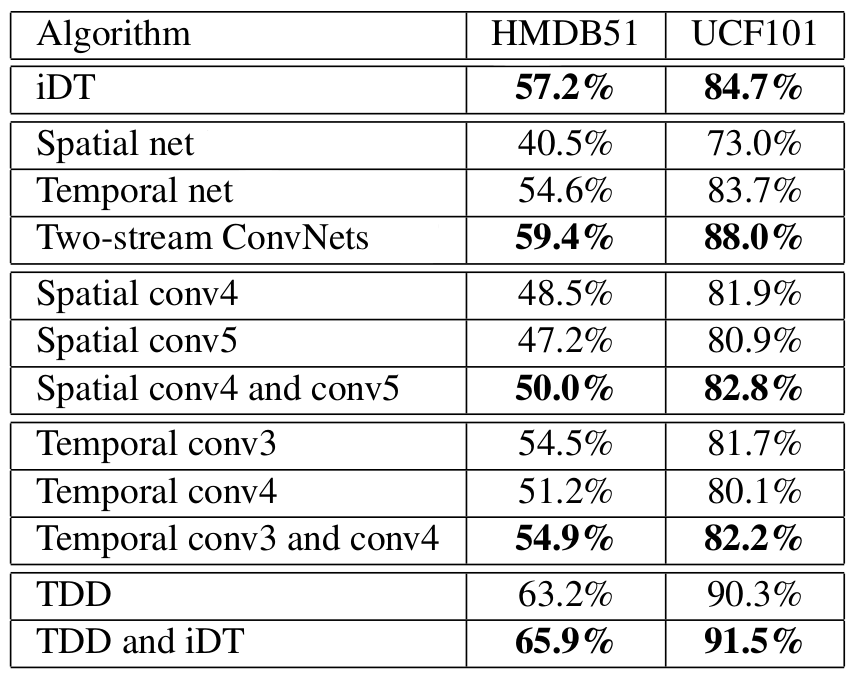
\includegraphics[width=0.5\textwidth]{img_deep/tdd_results}
    \caption{Action recognition performance of TDDs on HMDB51 and UCF101 compared to improved dense trajectories (iDT) \cite{wang_action_2013} and two-stream ConvNets \cite{simonyan_two-stream_2014}. \cite{wang_action_2015}}
    \label{tab:tdd_results}
\end{table}


\subsection{Generative Models}
\label{sec:generative}

TODO ??

One of the most popular deep learning models that can be trained unsupervised is the restricted Boltzmann machine [5]. A nice property of RBMs is that they can be greedily trained and stacked on top of each other to form deep belief networks (DBNs) [6], allowing us to learn representations of gradually increasing complexity. Training of these models using maximum likelihood learning is intractable, but they can be trained using contrastive divergence [4]. (Palasek Patras)

\textbf{Auto-Encoders:}\\
The most common architecture used is an auto-encoder
which learns representations based on its ability to recon-
struct the input images [35, 3, 49, 37]. Wang an Gupta (Unsupervised learning of visual representations using video.

\textbf{Restricted Boltzmann Machine:}\\
Boltzmann Machines are probabilistic networks, specifically undirected graphical models, that can learn the probability distribution inherent in a given dataset.
A Boltzmann Machine consists in its simplest form of two binary layers: A visible layer $x$ and a hidden layer $h$, which are fully connected to each other.
The Boltzmann Machine allows connections between units of the same layer, which renders training computationally extremely demanding.

The design of the Restricted Boltzmann Machine addresses this problem by restricting connections to nodes between different layers, which explains its name.
Restricted Boltzmann Machines can be trained using a Markov Chain Monte Carlo algorithm, namely Contrastive Divergence.

Once a Boltzmann Machine is trained, i.e.\ it learned the underlying probability distribution, data can be sampled from it.
The visible layer functions as both, input-layer during training and output-layer during sampling.

Restricted Boltzmann Machines can be trained with labeled as well as unlabeled data (supervised or unsupervised).

When training in an unsupervised manner, the RBM is able to learn feature representations of the inputs by mapping them onto activations of its hidden layer.
\ldots

When labeled data is present, the RBM can perform classification. 
For training, the labels are being concatenated with the input data and fed into the RBM.
A prediction for a given test example can then be obtained by using it as input for the RBM and sampling the model for the missing input, that was used for the labels during training.
The RBM then generates the most likely value for the missing label-input given the testing-input.

Restricted Boltzmann Machines correspond to feed-forward neural network models when reusing the learned weights in a topological equivalent NN model.
This is how unsupervised pre-training is conducted.

Models that can be trained in an unsupervised manner are especially attractive for the video-domain where labeling data is costly.

The RBM can be extended to process real-valued inputs.

Deep Belief Networks are stacked Restricted Boltzmann Machines.
In general the learning capacity of a single RBM is limited, but it can be increased by stacking multiple RBMs to form so called Deep Belief Network. (Lee)

\subsubsection{Unsupervised Learning of Video Representations using LSTMs (2015)}
\textcite{srivastava_unsupervised_2015} design recurrent neural network models based on Long-Short-Term-Memory cells (LSTMs) \cite{hochreiter_long_1997} for unsupervised learning of video representations from unlabeled video data.
They implement two LSTM networks in an auto-encoder setup: An encoder LSTM network maps input sequences of video frames to a fixed-length representation of hidden states, which is then decoded by another LSTM network to obtain a desired target sequence.

The authors consider three choices for the target sequence:
\begin{enumerate}
    \item The initial input sequence in reversed order (LSTM Auto-encoder model).
    \item A sequence of future inputs from the video, which were not presented to the encoder network before (LSTM Future Predictor model).
    \item A hybrid approach with two LSTM networks decoding the representation into both of these choices simultaneously (Composite model).
\end{enumerate}

Inputs to the LSTM encoder-network can be any kind of video representation, the authors evaluate raw image patches as well as high-level percepts, that are extracted by a convolutional neural network from the input. 

For a quantitative evaluation in a supervised setting, the models are first pre-trained in an unsupervised way and then fine-tuned for an action recognition task on the UCF-101 and HMDB-51 datasets.
Results of the purely unsupervised setting are evaluated qualitatively by printing and analysing decoded sequences.

The \textbf{LSTM Auto-encoder model}, as shown in figure \ref{fig:unsupervisedlstms_autoencoder}, consists of an encoder and a decoder LSTM network with parameters $W_1$ and $W_2$ respectively.
The encoder network is presented with one vector of the input sequence per timestep.
After the final input has been processed, the encoder's hidden state is used as a representation of the input.
The decoder network is then trained to translate the representation back into the initial input sequence, but in reversed order.
If the decoder is able to reconstruct the input sequence accurately from the representation, the essential information about the input must be encoded in the representation, which therefore is a good representation.

\begin{figure}[H]
    \centering
    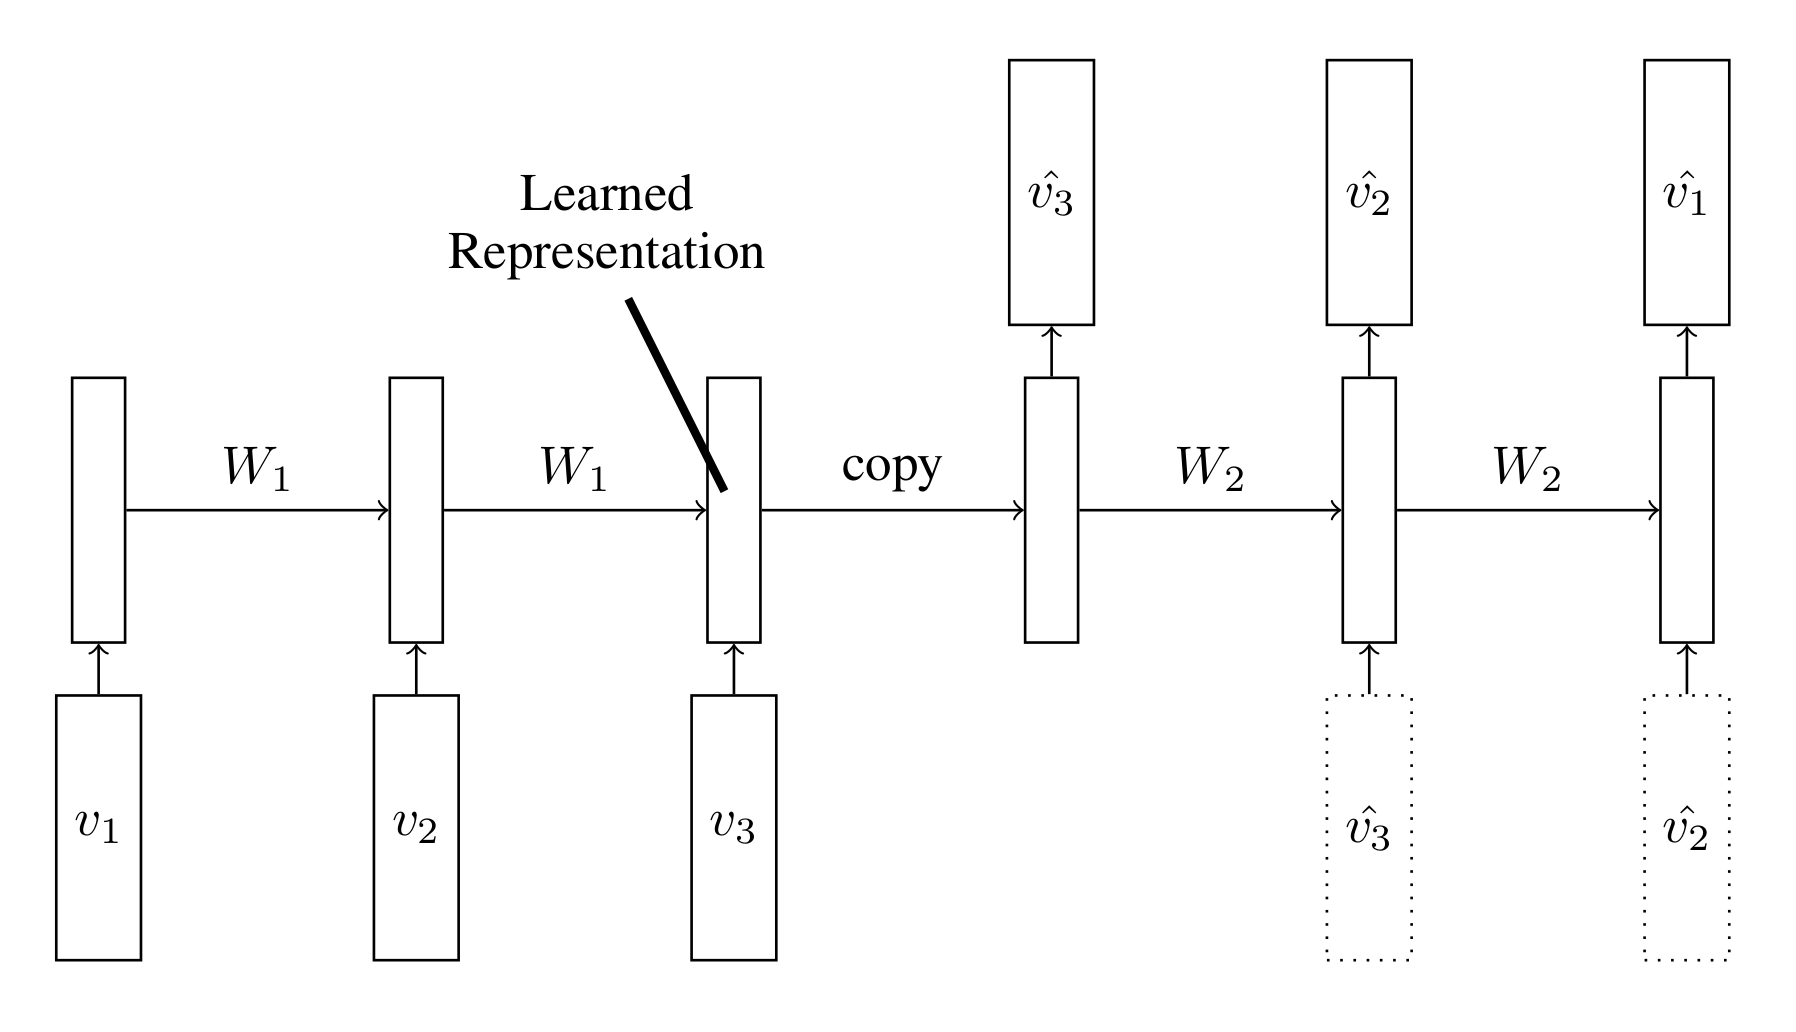
\includegraphics[width=0.7\textwidth]{img_deep/unsupervisedlstms_autoencoder}
    \caption{Auto-encoder model \cite{srivastava_unsupervised_2015}}
    \label{fig:unsupervisedlstms_autoencoder}
\end{figure}

The parameters of the LSTM networks $W_1$ and $W_2$ are, according to the network's recurrent nature, applied to its hidden state at timestep $i$, given an input $v_i$ of the input sequence $\{v_1, \cdots, v_T\}$ of length $T$.
The outputs of the decoder network $\hat{v}_i,\ i \in \{1,\cdots,T\}$ correspond to the decoded input sequence in reversed order.
The decoder network can be \textit{conditional}, i.e.\ it receives its last generated output as input (dotted boxed in figure \ref{fig:unsupervisedlstms_autoencoder}).

The \textbf{LSTM Future Predictor model} also consists of two recurrent LSTM networks but predicts frames that continue the previously presented input sequence.
The architecture, as shown in figure \ref{fig:unsupervisedlstms_futurepredictor}, is the same as for the Auto-encoder model.
This decoder LSTM network can also be \textit{conditional} or \textit{unconditioned}.

\begin{figure}[H]
    \centering
    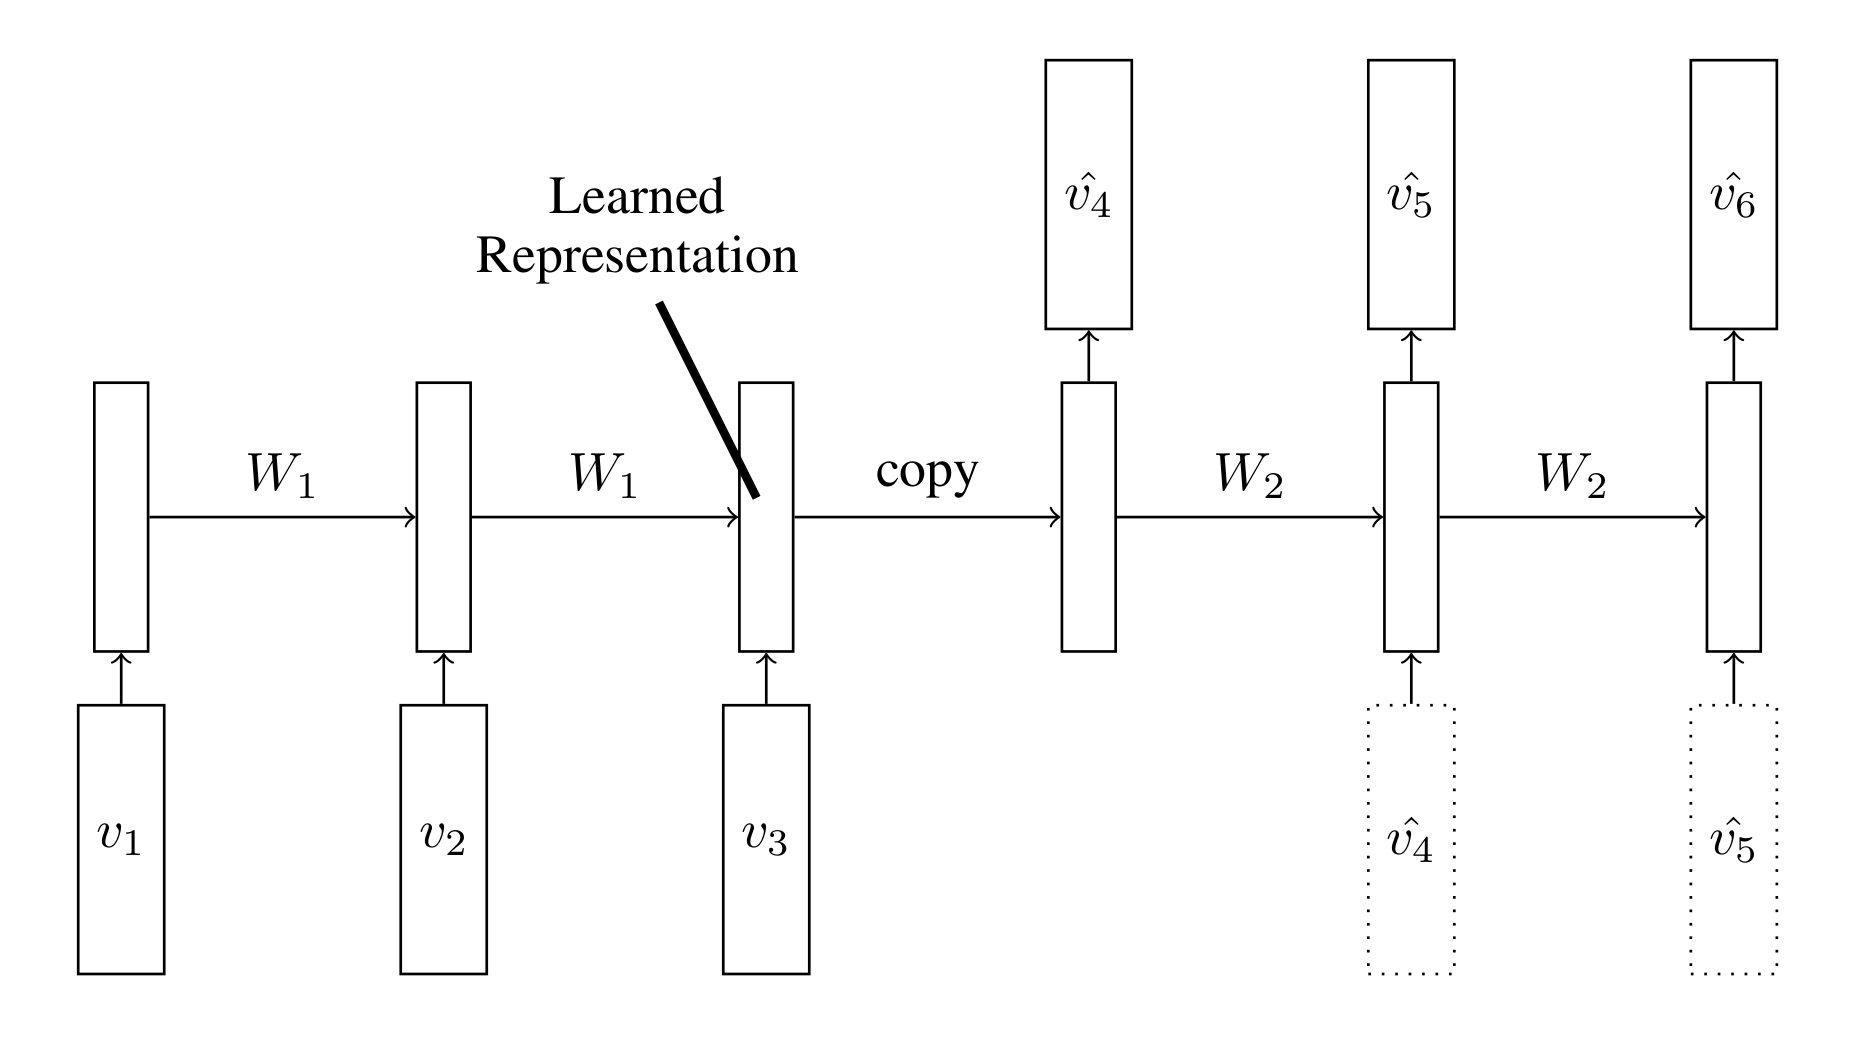
\includegraphics[width=0.7\textwidth]{img_deep/unsupervisedlstms_futurepredictor}
    \caption{Future-predictor model \cite{srivastava_unsupervised_2015}}
    \label{fig:unsupervisedlstms_futurepredictor}
\end{figure}

The \textbf{Composite model} consists of an encoder LSTM network and two decoder LSTM networks, which reconstruct the original input sequence and predict future frames simultaneously.
This model tries to overcome the disadvantages that each of the single models have: A high-capacity auto-encoder tends to simply memorize the inputs, while a future predictor tends to store information about just the last few frames of the input, because those are needed most for future prediction.
The composite model, as shown in figure \ref{fig:unsupervisedlstms_composite}, therefore puts additional constraints on the encoder networks, i.e.\ the learned representation must be suitable for both tasks.

\begin{figure}[H]
    \centering
    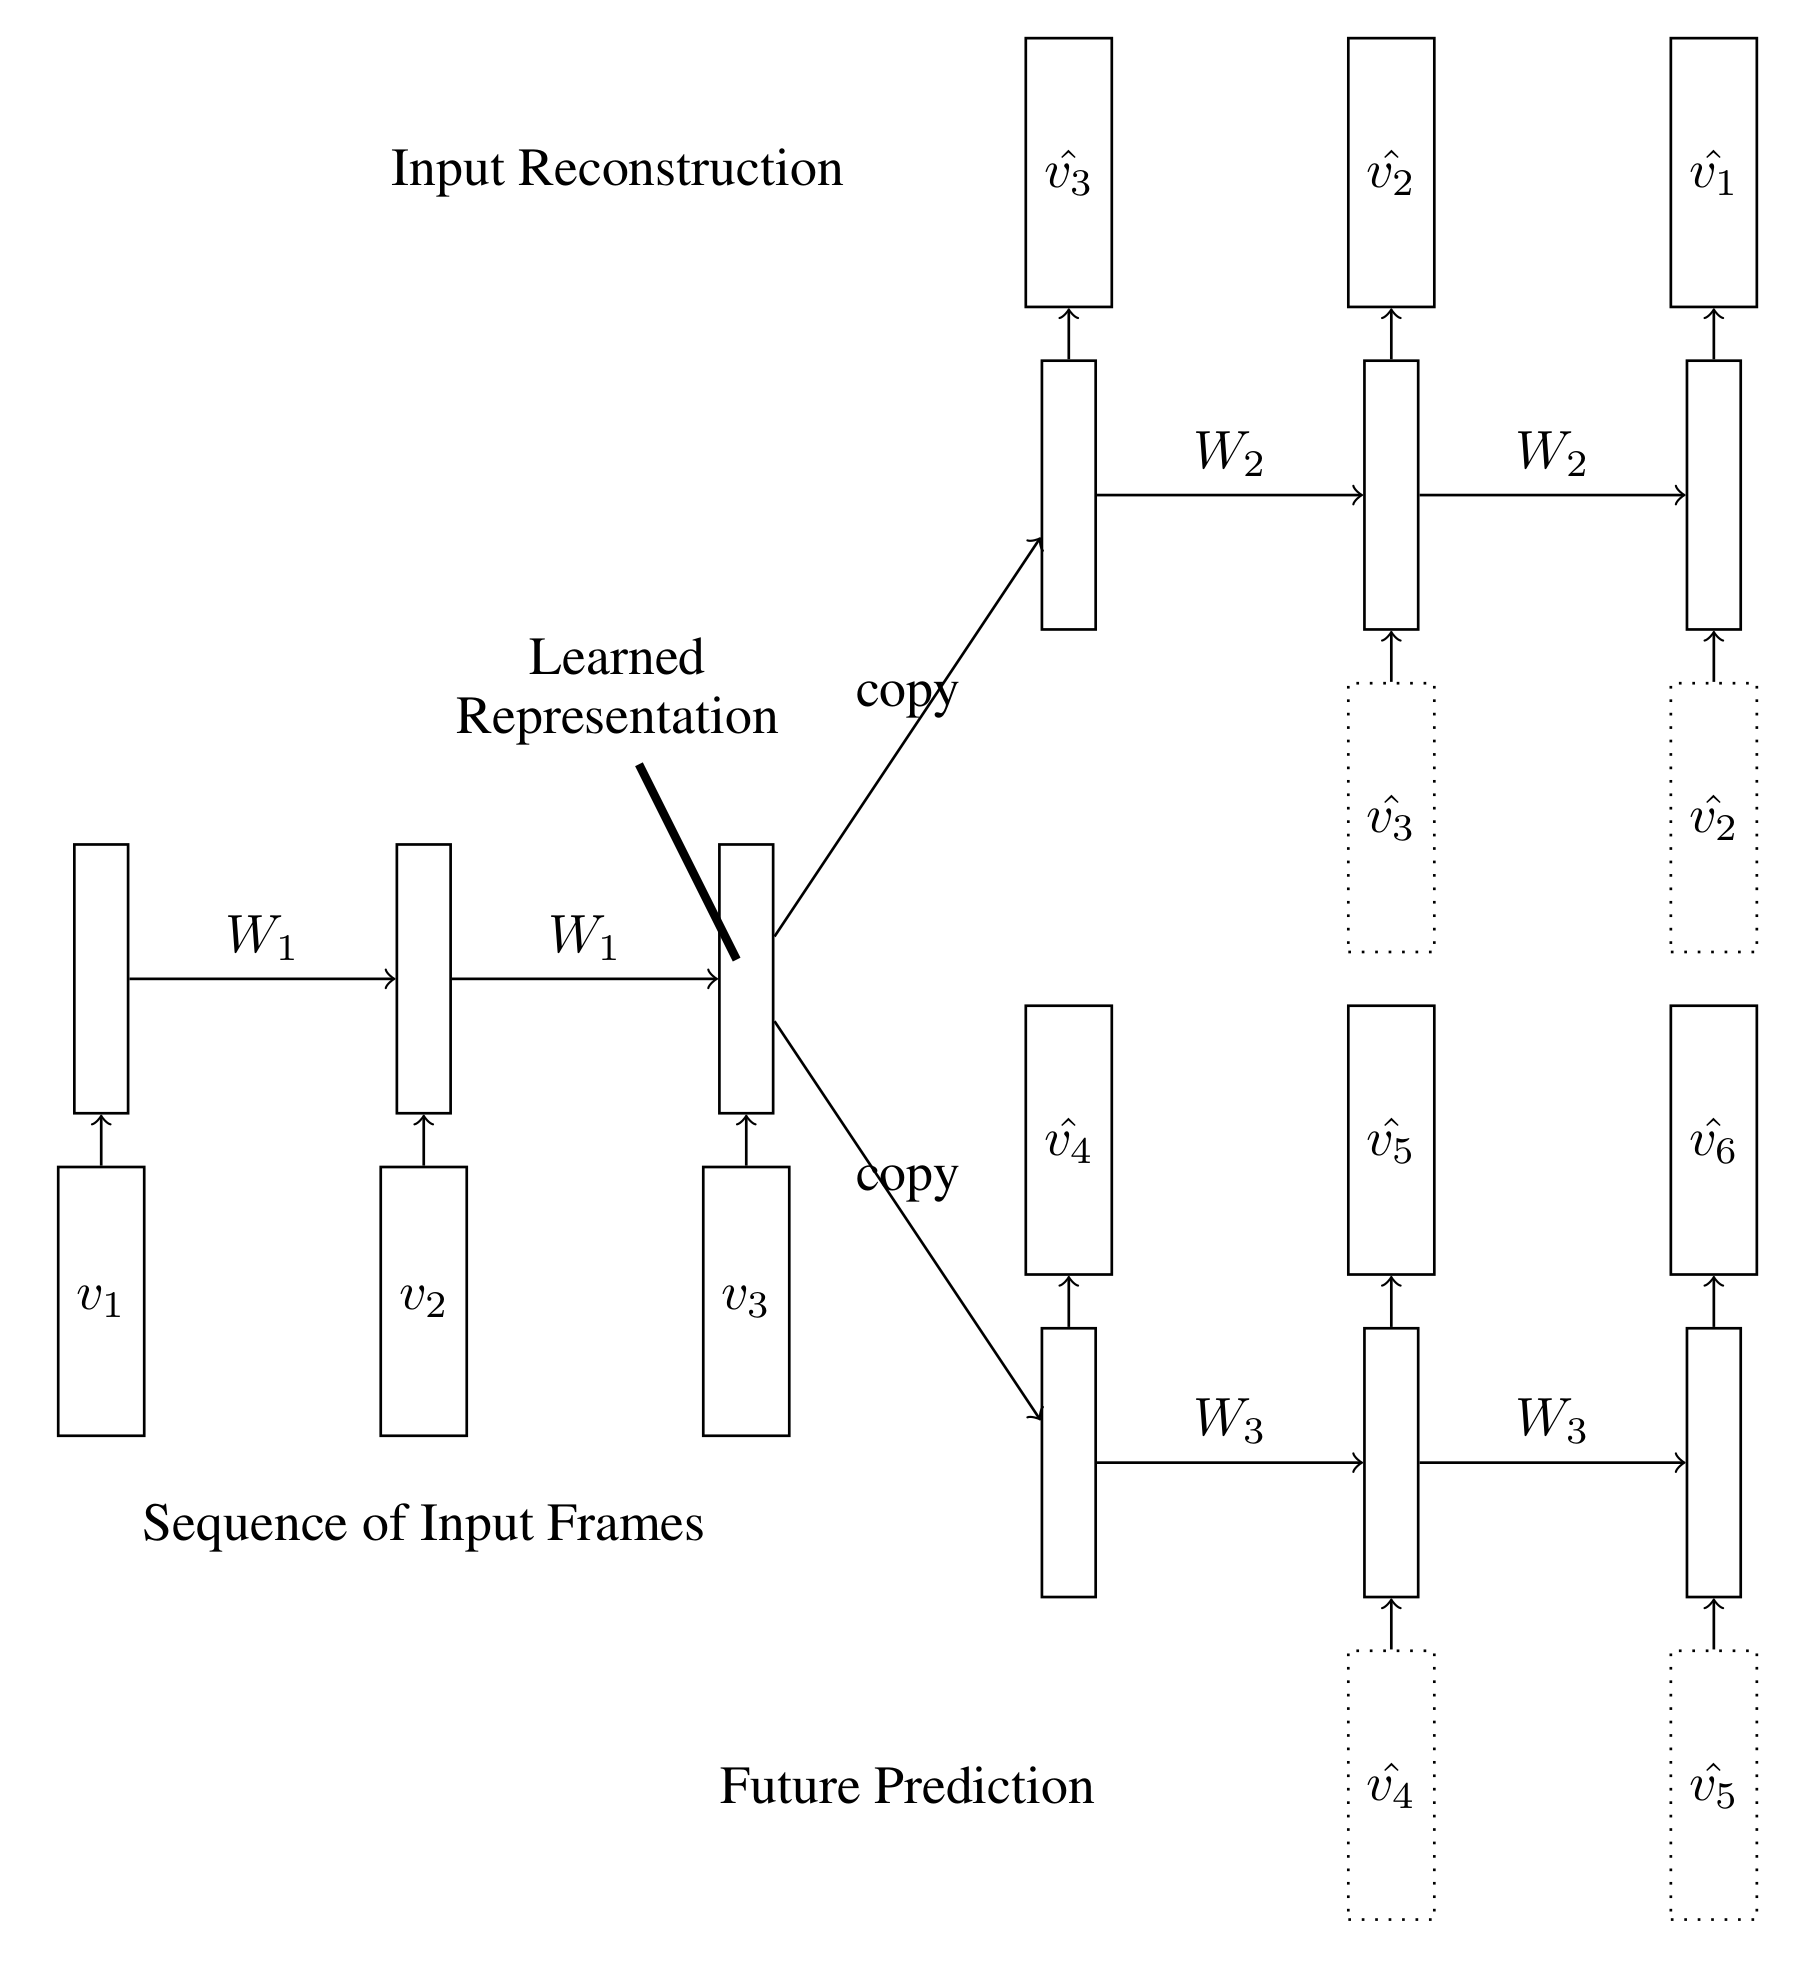
\includegraphics[width=0.7\textwidth]{img_deep/unsupervisedlstms_composite}
    \caption{Composite model \cite{srivastava_unsupervised_2015}}
    \label{fig:unsupervisedlstms_composite}
\end{figure}

\textcite{srivastava_unsupervised_2015} provide a qualitative analysis of the composite model by visualising its outputs.
The model, separately evaluated for one and two layers of $2048$ LSTM units each, is trained on 10 frames of synthetically composed video-data consisting of two moving MNIST digits in a $64 \times 64$ pixel area.
The digits can be superimposed and bounce off the walls.
The results for image reconstruction and future prediction are shown in figure \ref{fig:unsupervisedlstms_movingmnist}.

\begin{figure}[H]
    \centering
    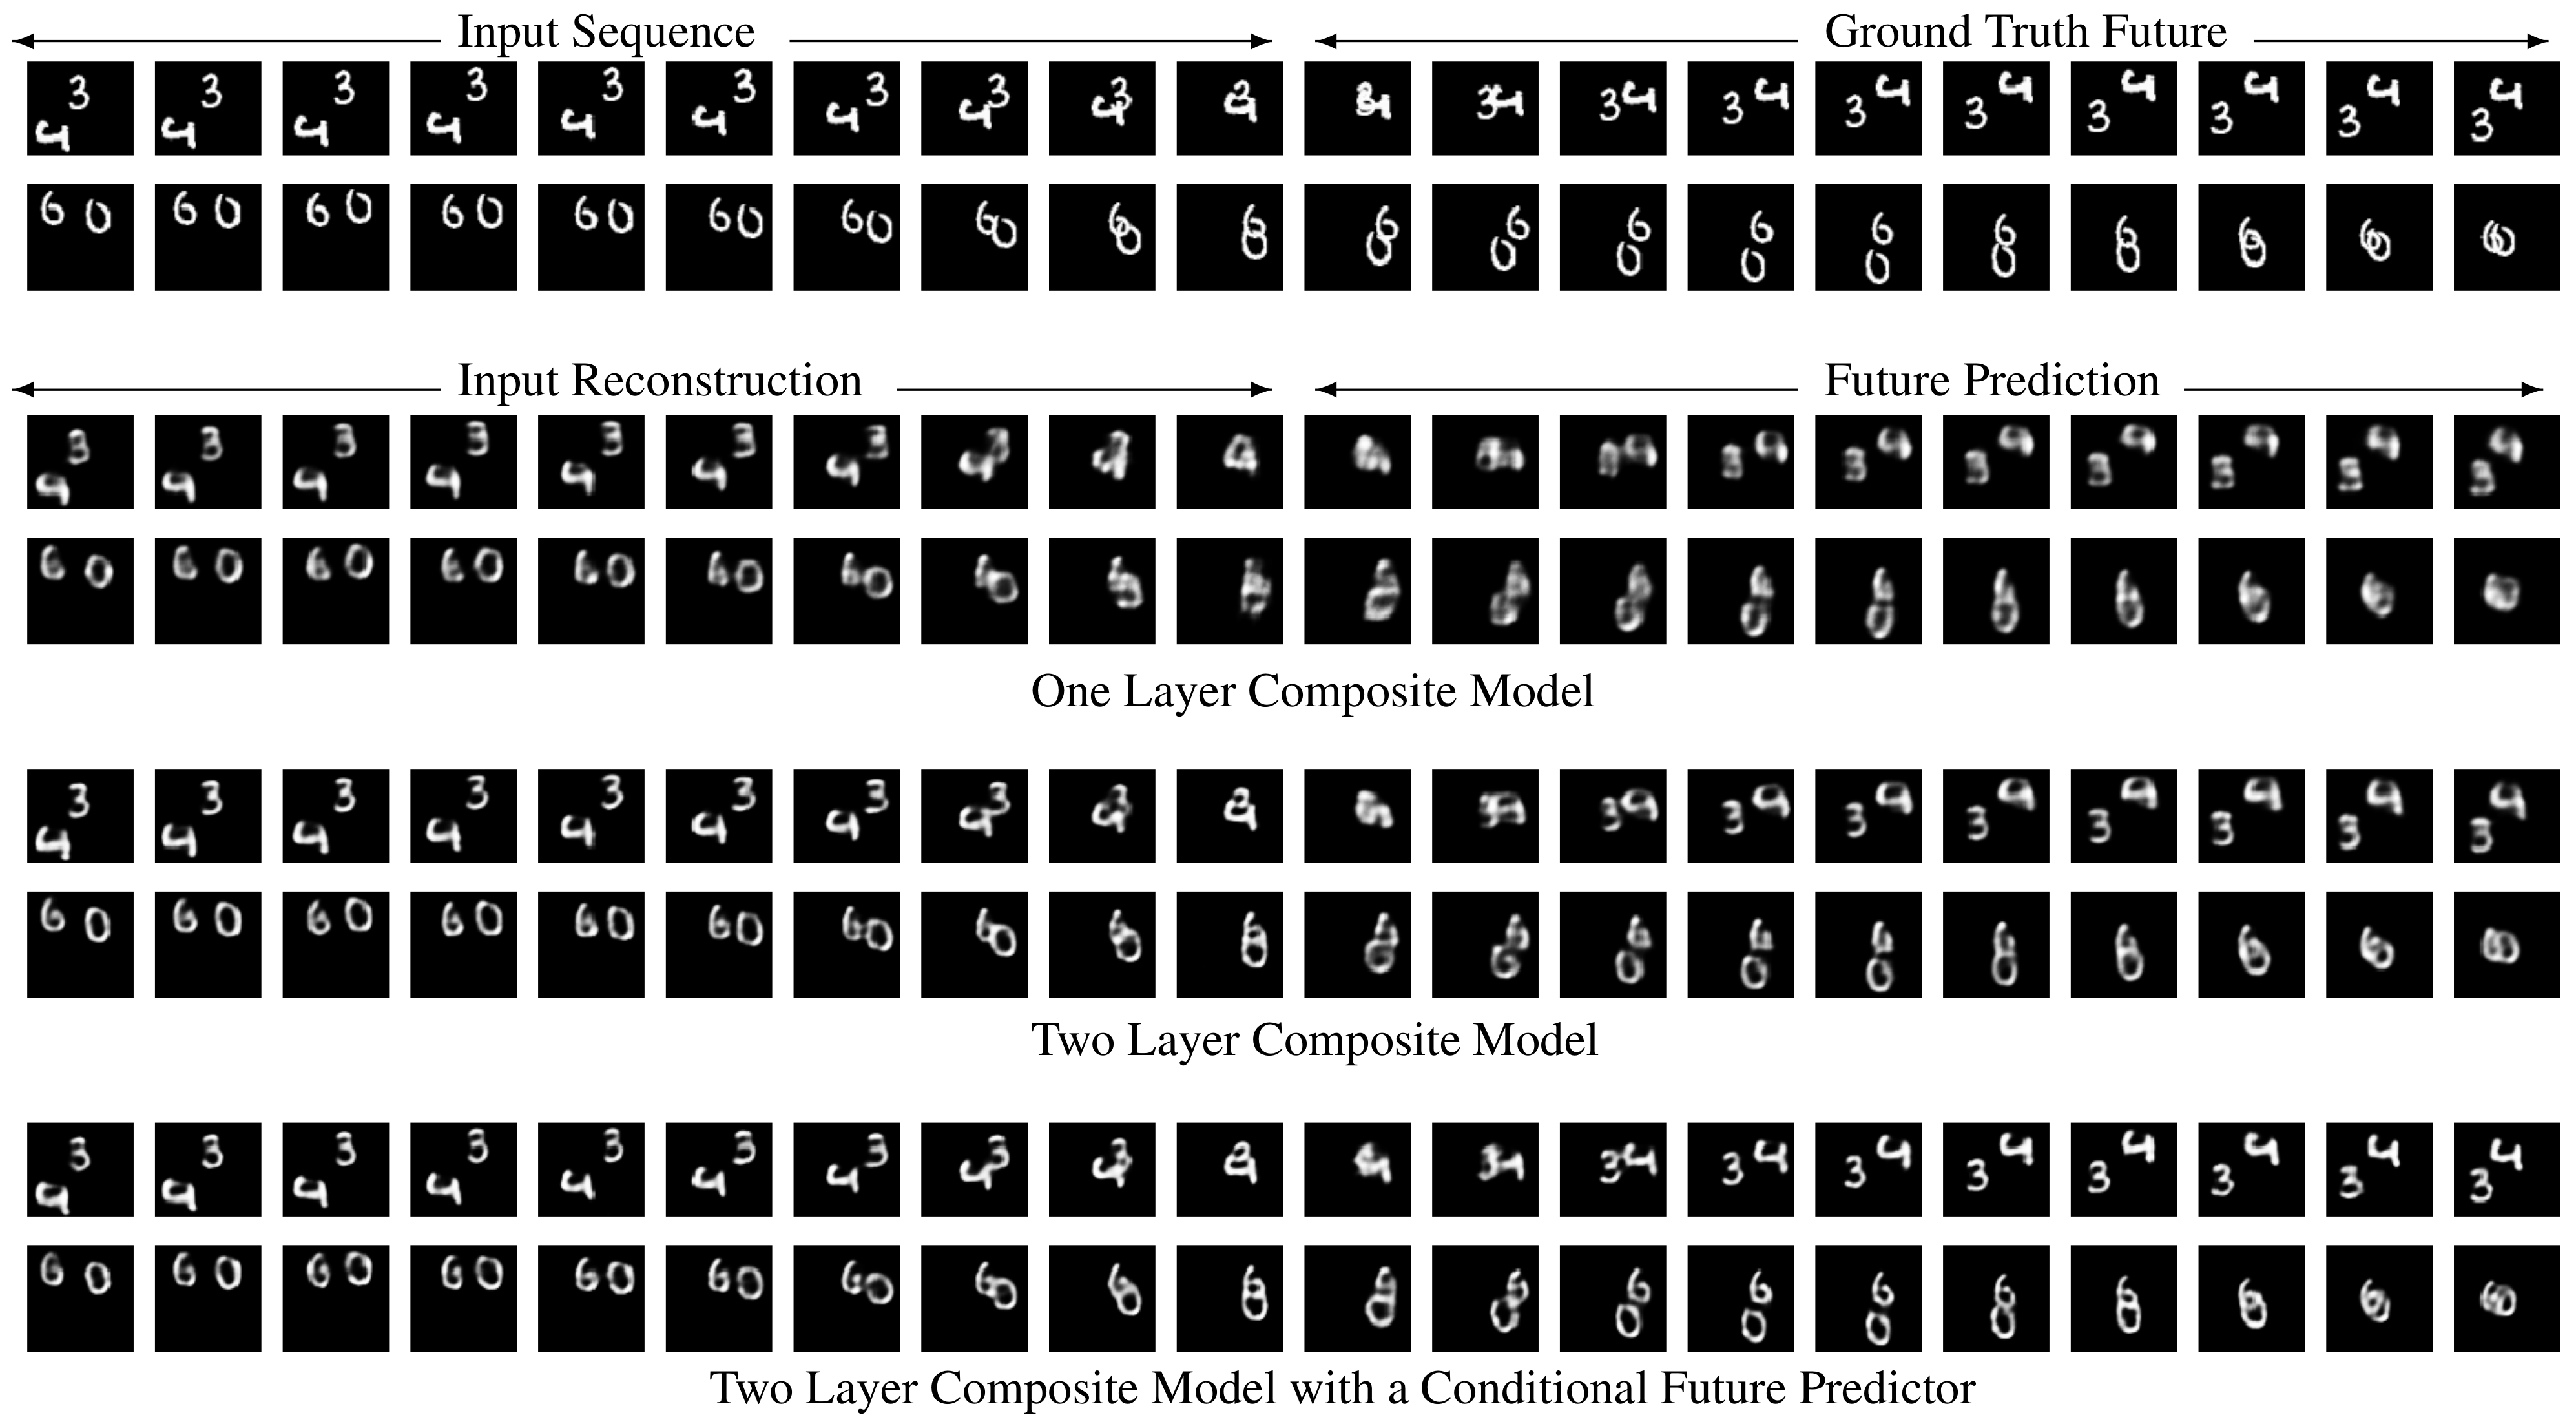
\includegraphics[width=\textwidth]{img_deep/unsupervisedlstms_movingmnist}
    \caption{Input reconstruction and future predictions of composite models on a synthetic dataset of moving MNIST digits. \cite{srivastava_unsupervised_2015}}
    \label{fig:unsupervisedlstms_movingmnist}
\end{figure}

The first row of figure \ref{fig:unsupervisedlstms_movingmnist} shows the 10 frame input sequence and the following 10 future frames.
The model is able to make fairly good predictions on this dataset.
Adding a second layer of LSTM units and making the future predictor conditional further improves the predictions.
When applying the model on $32 \times 32$ natural image patches of real-life videos from the UCF-101 dataset, results show however, that the future prediction quickly blurs out as illustrated in figure \ref{fig:unsupervisedlstms_ucfpatches}.

\begin{figure}[H]
    \centering
    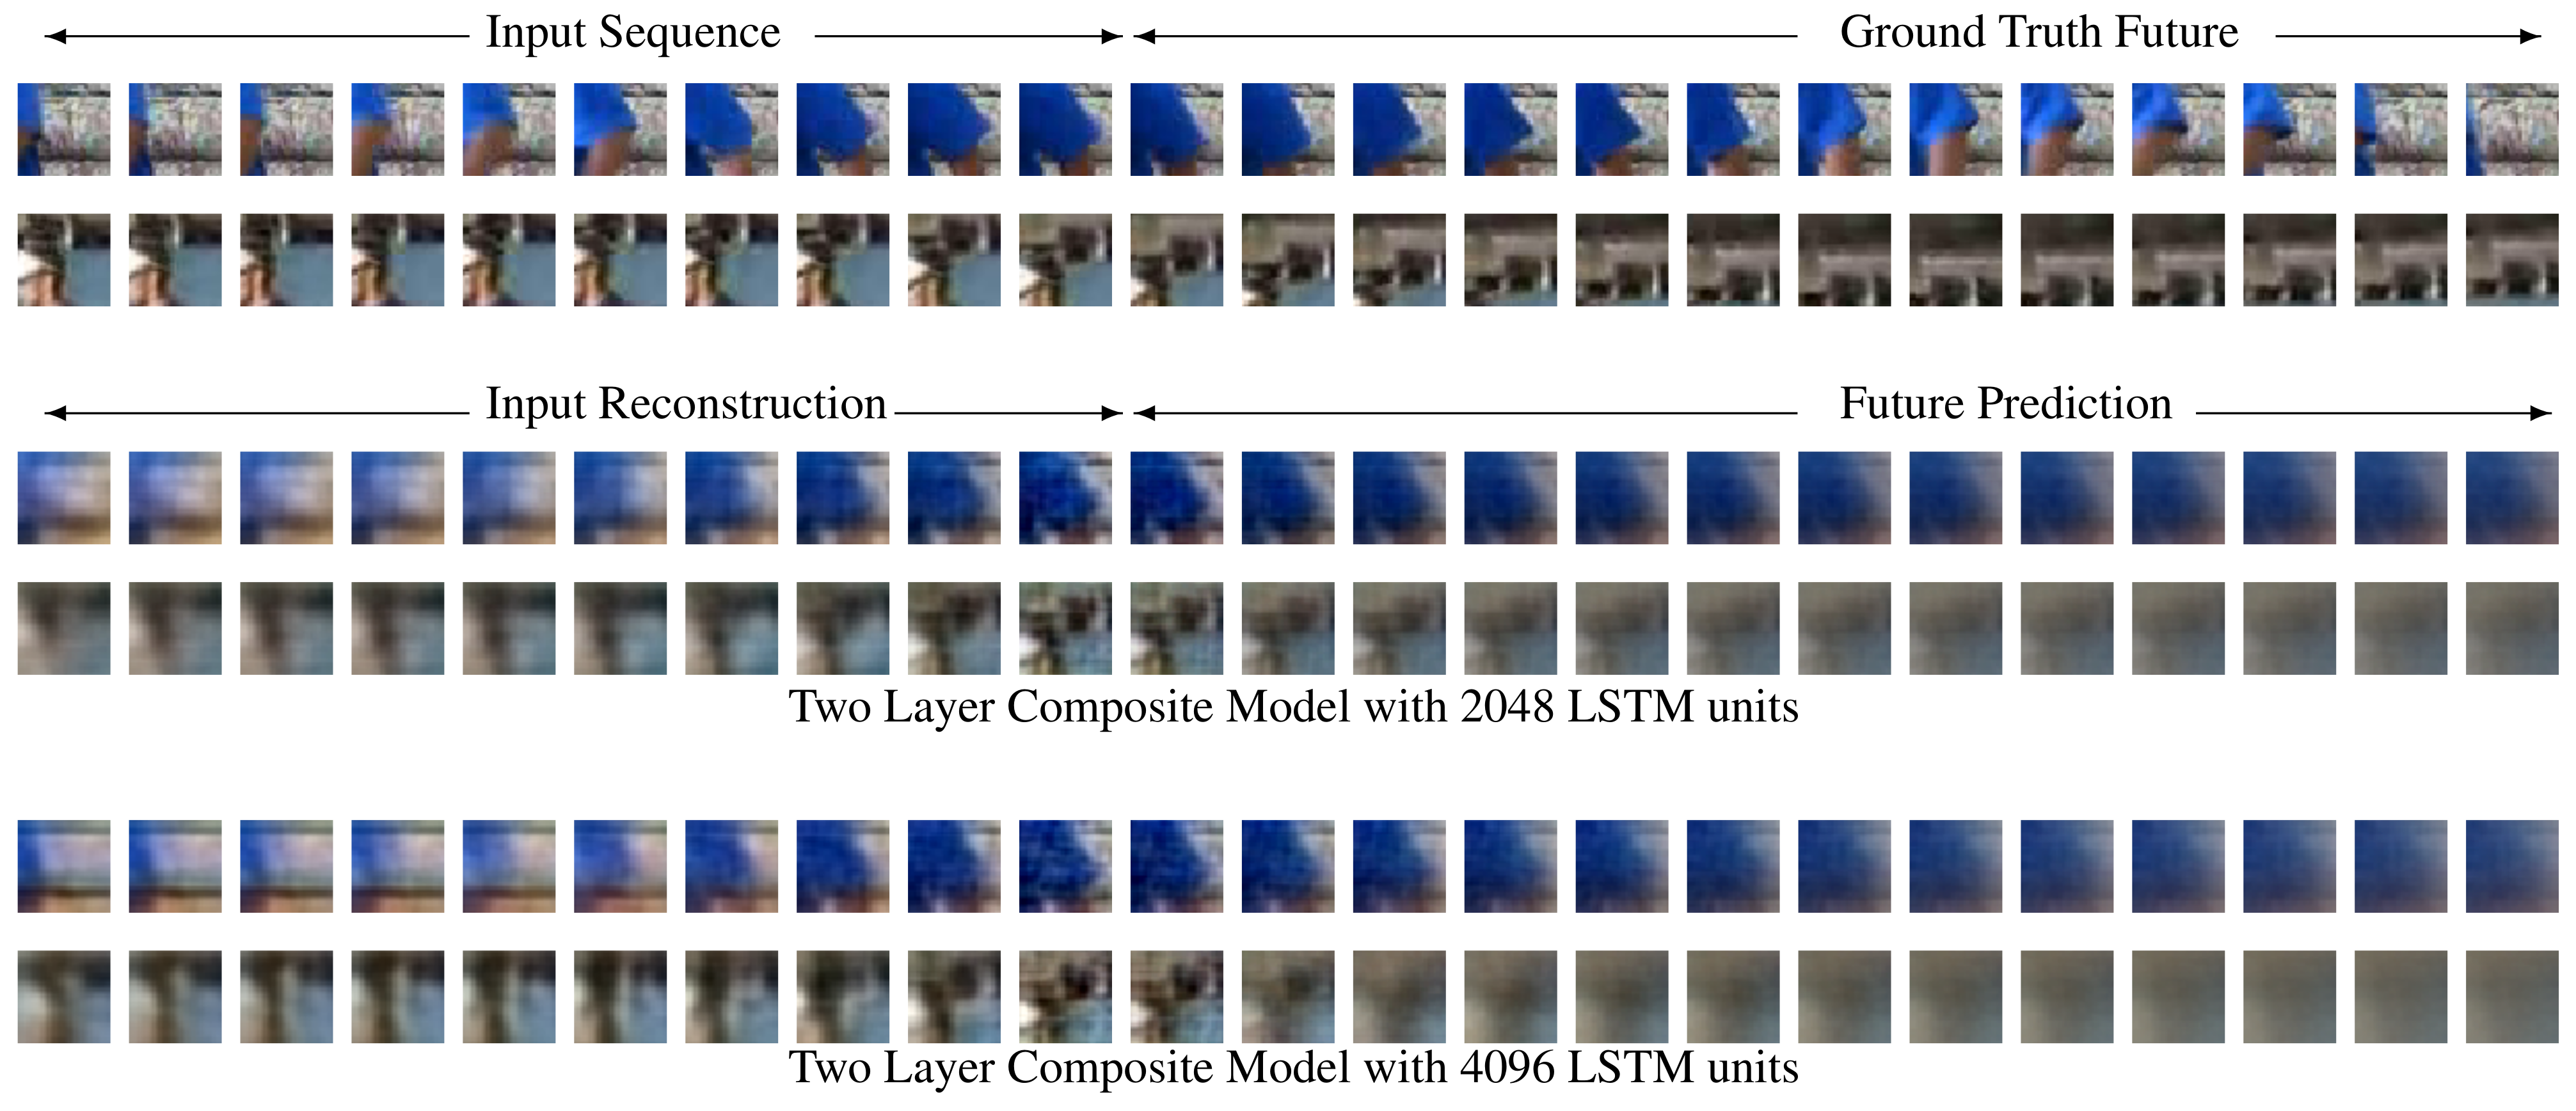
\includegraphics[width=\textwidth]{img_deep/unsupervisedlstms_ucfpatches.png}
    \caption{Image reconstruction and future prediction of a two-layer composite model with a different number of LSTM units in each layer. \cite{srivastava_unsupervised_2015}}
    \label{fig:unsupervisedlstms_ucfpatches}
\end{figure}

The authors evaluate the effectiveness of features obtained from unsupervised learning for supervised action recognition:

\begin{enumerate}
    \item A two layer model with $2048$ LSTM cells in each layer is trained in an unsupervised way on 300 hours of video, randomly sampled from the Sports-1M dataset.
        The model is trained to autoencode 16 frames and predict 13 frames.
    \item Once training is finished, a LSTM network as shown in figure \ref{fig:unsupervisedlstms_classifier} is initialized with the weights learned by the composite model.
    \item Depending on the used benchmark, this LSTM network is then fine-tuned on either UCF-101 or HMDB-51 to function as a supervised classifier.
\end{enumerate}

The model is designed to use center crops of size $224 \times 224$ from the datasets or high-level optical-flow percepts, i.e.\ activations of a temporal stream CNN as in \cite{simonyan_two-stream_2014}, as inputs.

\begin{figure}[H]
    \centering
    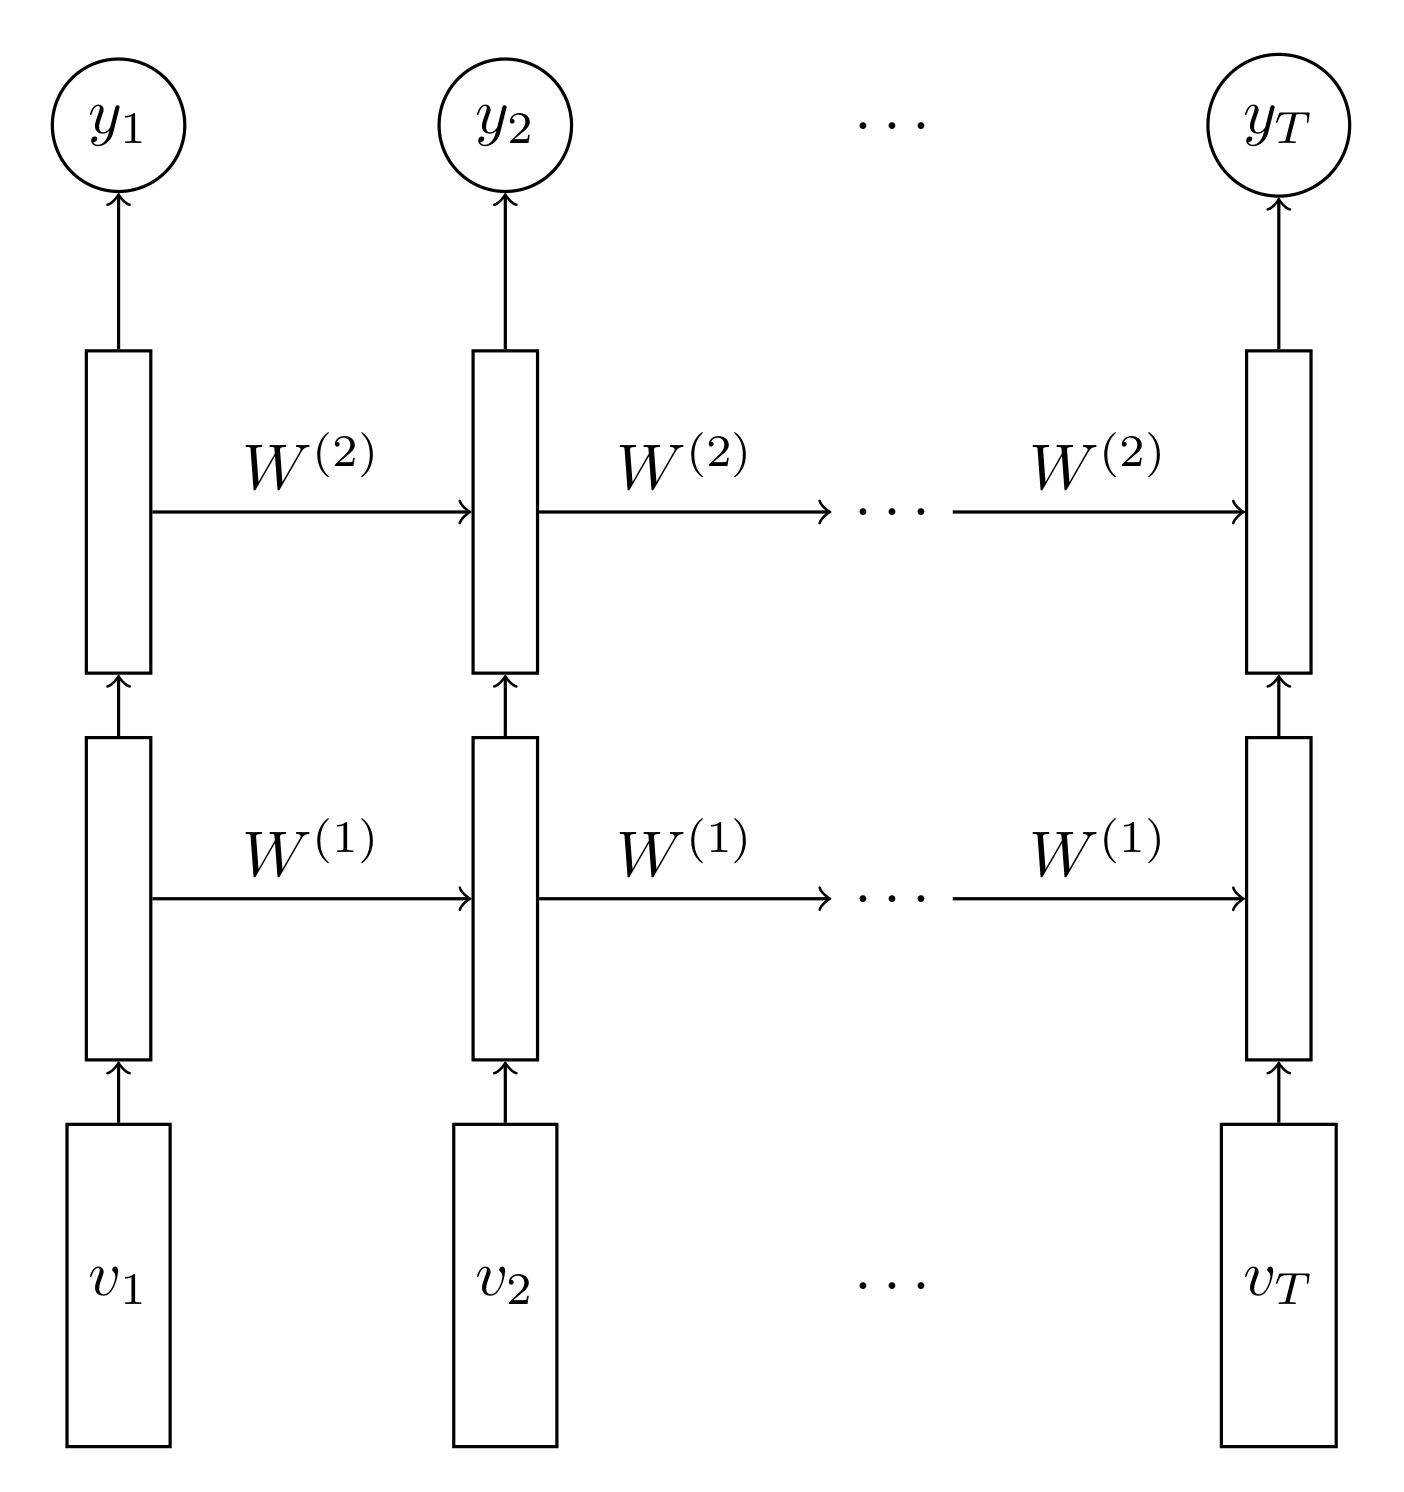
\includegraphics[width=0.5\textwidth]{img_deep/unsupervisedlstms_classifier}
    \caption{Recurrent LSTM classifier unfolded in time with input sequence $\{v_1, \cdots, v_T\}$ \cite{srivastava_unsupervised_2015}}
    \label{fig:unsupervisedlstms_classifier}
\end{figure}

Baseline method involves initializing the model with random weights.
The results as given in table \ref{tab:unsupervisedlstms_results} show, that initializing the model with features obtained from unsupervised learning increases the performance significantly, when only very few training examples per class are available (improvement of about $5\%$).
With more available labeled data, the improvement becomes smaller (about 1\%).

\begin{table}
    \centering
    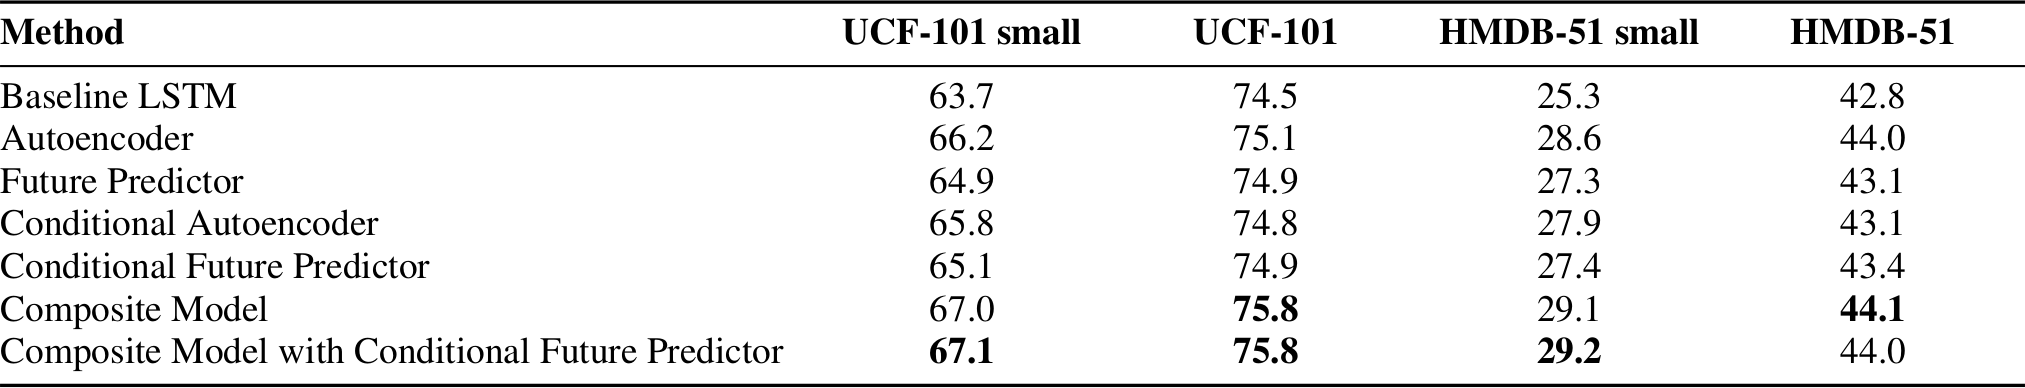
\includegraphics[width=\textwidth]{img_deep/unsupervisedlstms_results}
    \caption{Comparison of unsupervised pre-training methods for an two-layer LSTM classifier. The small versions of benchmarking datasets are subsets containing only 10 (UCF-101) and 4 (HMDB-51) action videos per class. \cite{srivastava_unsupervised_2015}}
    \label{tab:unsupervisedlstms_results}
\end{table}

The authors conclude: Pre-training models on just unrelated datasets (here 300 hours of YouTube videos) can increase action recognition performance.
Unsupervised learning gives a significant improvement if only few labeled training examples are available.


\subsubsection{Action Recognition Using Convolutional Restricted Boltzmann Machines (2016)}
%\cite{palasek_action_2016}
\textcite{palasek_action_2016} apply Convolutional Deep Belief Networks (ConvDBNs) for learning video representations in an unsupervised fashion in order to perform human action recognition.
ConvDBNs are generated by stacking layers of Convolutional Restricted Boltzmann Machines (ConvRBMs) \cite{lee_convolutional_2009-1}.
The ConvRBM was initially proposed by \textcite{lee_convolutional_2009-1} to address several problems that occur when applying RBMs and DBNs to images:

\begin{enumerate}
    \item Realistic images are high-dimensional and DBNs do not scale well with the input size. \cite{lee_convolutional_2009-1} 
    \item DBNs do not take the special structure of images into account, specifically that objects can occur in any area of an image. Feature extractors therefore have to be learned for each location in the image separately. \cite{lee_convolutional_2009-1} 
\end{enumerate}

Equivalently to Convolutional Neural Networks, the Convolutional Restricted Boltzmann Machine uses weight-sharing and pooling to make the detection of a specific feature in an input image translationally invariant.

The basic \textbf{ConvRBM} architecture is shown in figure \ref{fig:convrbm_architecture}.
It has the following properties:\cite{lee_convolutional_2009-1}

\begin{figure}[H]
    \centering
    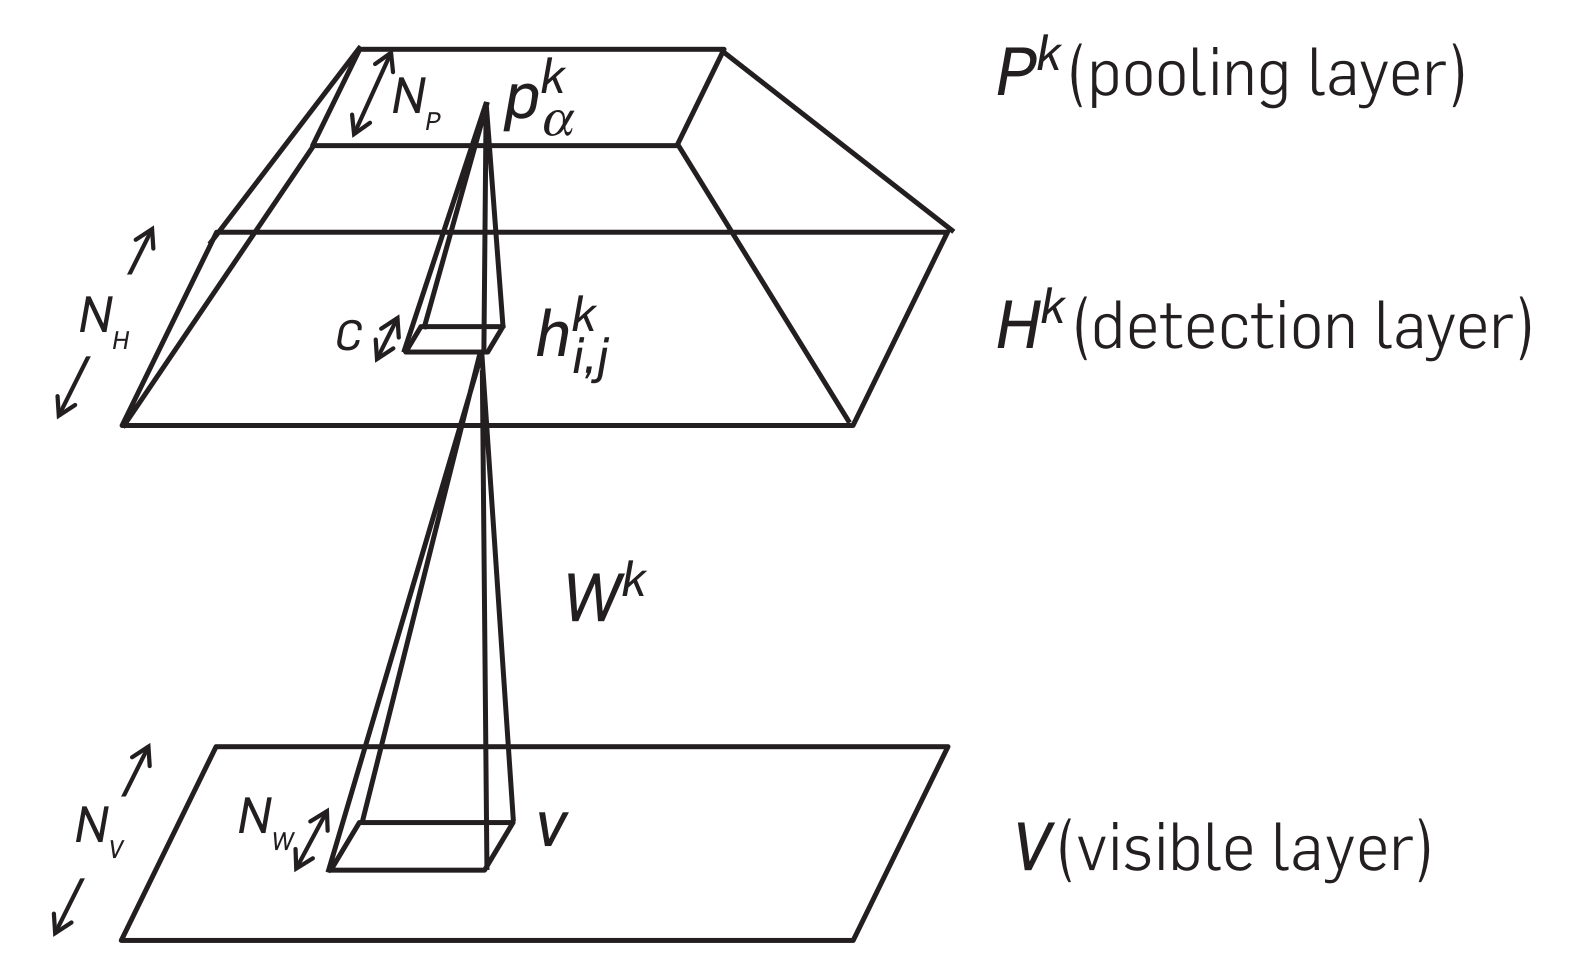
\includegraphics[width=0.6\textwidth]{img_deep/convrbm_architecture}
    \caption{Architecture of the Convolutional Restricted Boltzmann Machine. The figure shows group $k$ in the detection- and pooling-layer. \cite{lee_convolutional_2009-1}}
    \label{fig:convrbm_architecture}
\end{figure}

\begin{itemize}
    \item The visible layer $V$ consists of binary input units, but can be easily modified to handle real-valued inputs.
    \item The hidden layer $H$ consists of $K$ groups, with a filter $W^k$ belonging to each group ($k \in \{1,\cdots, K\}$).
        To illustrate the equivalency to CNNs, which consists of detection and pooling layers, the hidden layer is denoted as \textit{detection layer} in figure \ref{fig:convrbm_architecture}.
    \item A group corresponds to a feature map in CNNs, i.e. the activations produced by a convolutional filter.
    \item The filter weights define the connections between a local patch in the visible layer and a hidden unit in the detection layer of the filter's group.
    \item All hidden units in the detection layer of a group are connected to their local patches by the same filter weights, i.e\ the filters in a group share weights.
    \item The hidden units share a bias $b_k$ per group and all visible units have a single bias $c$.
\end{itemize}

To form a more expressive deep architecture, called Convolutional Deep Belief Networks (ConvDBNs), layers of ConvRBMs are stacked.
Probabilistic max-pooling is used to reduce the dimensionality of each hidden (detection) layer.
Since regular max-pooling was designed for deterministic models such as CNNs, a probabilistic max-pooling method is derived, in order to enable full probabilistic inference in the model.
In probabilistic max-pooling, only one unit in the input patch of the pooling operation is allowed to be active.
The output unit is active, if and only if one unit in the input patch is active.
Pooling operations are needed, to feed progressively more information to higher-level feature detectors and to make high-level representations invariant to translations of features in the lower layers. \cite{lee_convolutional_2009-1}

The energy function of the ConvDBN is defined by summing the energy functions of the individual ConvRBMs.
ConvDBNs can be trained in a greedy, layer-wise way: After a ConvRBM layer is trained individually, its weights are frozen and its activations in the hidden/detection layer are taken as inputs for the following layer.
\cite{lee_convolutional_2009-1}

\textcite{palasek_action_2016} apply three stacked ConvRBMs (a ConvDBN) to action recognition.
They use the Gaussian-Bernoulli version of ConvRBMs, which is the real-valued extension of regular binary ConvRBMs, to extract features from still video frames and aggregate them into a video representation that can be classified using a SVM.

Different configurations for the layers in the ConvDBN are being evaluated:
\begin{description}
    \item[First layer ConvRBM] \hfill \\
        Either $32$ or $64$ filters sized $5 \times 5$ or $3 \times 3$ pixels.\\
        Optional probabilistic max-pooling layer with patch size of $2 \times 2$ units.
    \item[Second layer ConvRBM] \hfill \\
        Contains $64$ filters of size $3 \times 3$
        Optional probabilistic max-pooling layer with patch size of $2 \times 2$ units.
    \item[Third layer ConvRBM] \hfill \\
        Contains $128$ filters of size $3 \times 3$ pixels.
        Optional probabilistic max-pooling layer with patch size of $2 \times 2$ units.
\end{description}

The approach for generating fixed length video representations for variable sized input videos is shown in figure \ref{fig:palasekpatras_approachschematik}.

\begin{figure}[H]
    \centering
    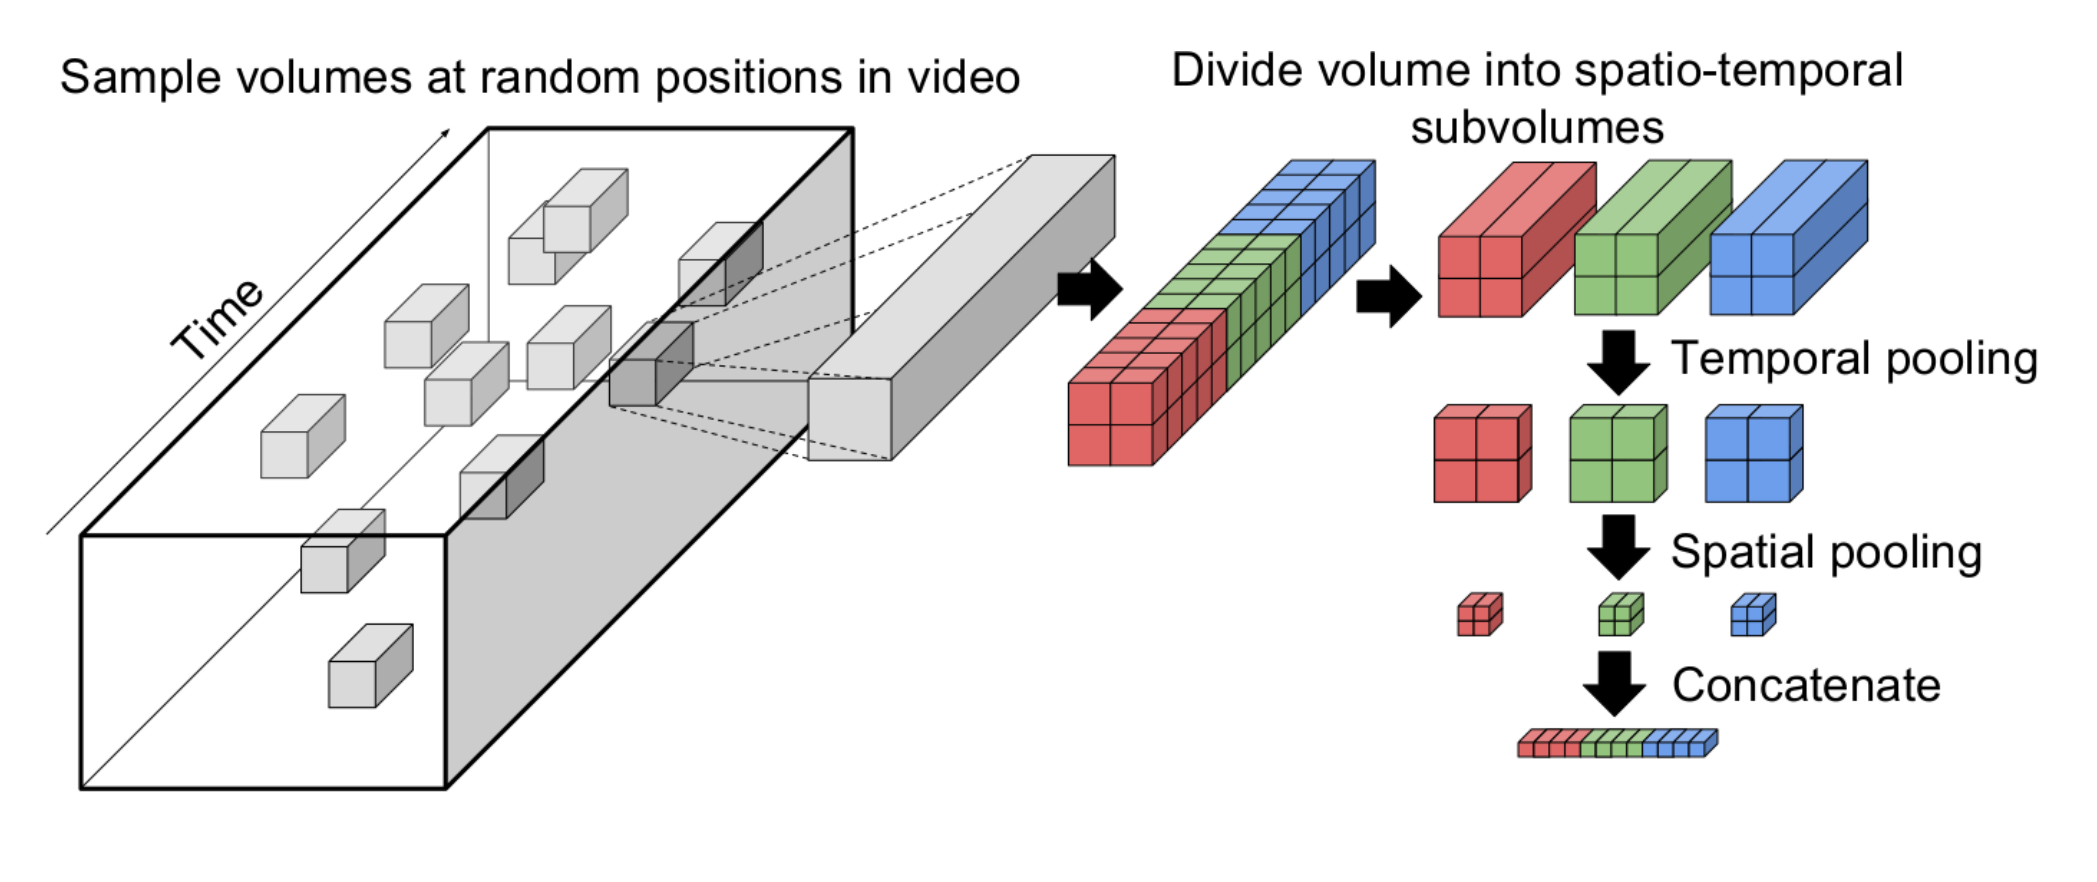
\includegraphics[width=\textwidth]{img_deep/palasekpatras_approachschematik}
    \caption{Approach for generating fixed sized video-representations using ConvDBN activations. An input video is handled as video-volume of stacked frames. \cite{lee_convolutional_2009-1}}
    \label{fig:palasekpatras_approachschematik}
\end{figure}

Given an input video, interpreted as a volume of stacked video frames, subvolumes of size $32 \times 32$ pixels and with a length of $15$ frames are extracted at random positions.
Each subframe is fed individually into the ConvDBN and the resulting activations of one of its layers are extracted.
The activations of all subframes are stacked to form a feature representation of the subvolume.
This feature representation is then divided into $2 \times 2 \times 3$ parts, mean-pooled along the temporal dimension, spatially pooled and concatenated to form the final representation of the given subvolume (see figure \ref{fig:palasekpatras_approachschematik}). \cite{lee_convolutional_2009-1}

A Gaussian Mixture Model is trained on all the extracted feature representations to encode them into a Fisher Vector representation of the video.
These Fisher Vectors can then be classified using a SVM, as in approaches that use hand-crafted local features (see section \ref{chap:conventional}).
 
\textcite{palasek_action_2016} evaluated their approach using the activations of different ConvDBN layers as features.
The ConvDBN is trained in an unsupervised way on grayscaled, static video-frames of the UCF-101 dataset, which contains a total of $1,700,000$ frames.
For each of the 9537 training videos UCF-101 dataset, $1000$ subvolumes are extracted as training inputs for the ConvDBN.

Activations from the first pooling layer worked best and yield an accuracy of $55.06\%$ in the overall approach.
Although, the results are not competitive to other state-of-the-art approaches reported previously in this work, the experiments were conducted to compare the performance of features learned in an unsupervised manner to hand-crafted features.

The authors also evaluated incorporating HOG features in their experimental setup and achieved significantly worse results: $50.75\%$.
They therefore argue, that features learned in an unsupervised way are more descriptive than hand-crafted features for human action recognition from video.

The authors showed, that features learned from video data in an unsupervised way is able to outperform hand-crafted features.
The overall performance, that is action recognition accuracy of $55.06\%$ on UCF-101, is rather weak compared to other approaches.
This probably stems from the fact, that features were learned from static frames only, instead of incorporating motion information.

\subsection{Temporal Coherency Networks}
%\subsubsection{Unsupervised learning of spatiotemporally coherent metrics -- Goroshin et al. (2015)}
%cite{goroshin_unsupervised_2015}
%subsubsection{Unsupervised learning of visual representations using videos -- Wang and Gupta (2015)}
%cite{wang_unsupervised_2015}

\subsubsection[Shuffle and Learn: Unsupervised Learning using Temporal Order Verification (2016)]{Shuffle and Learn: Unsupervised Learning using Temporal Order Verification -- Misra et al. (2016)}
%\cite{misra_shuffle_2016}
\textcite{misra_shuffle_2016} propose an efficient method for learning video representations based on temporal order verification.
Temporal order verification is a binary classification task.
Given a sequence of video frames, a classifier has to determine whether the sequence is in correct temporal order.
Datasets to train and test such a classifier can be easily generated by sampling short sequences of frames from a video and exchanging frames in some of them.

In the strictest sense, using temporal order verification for representation learning is not an unsupervised method, since the labels \textit{correct temporal order} and \textit{incorrect temporal order} are learned for input sequences.
The authors argument however, that obtaining the label is free and the method can therefore be attributed as unsupervised.

Forcing an algorithm to reasoning about the temporal order of frames, produces a representation that captures the motion of persons and objects in the scene, since they define the temporal order.
A resulting video representation therefore embeds information that is most vital for accurate action recognition.

The authors evaluate this approach using a Convolutional Neural Network, that is applied to a sequence of three frames in parallel.
Input sequences of three frames are used, since four or five frames did not yield a significant improvement in performance.
Results are obtained on the UCF-101 and HMDB-51 benchmark dataset.

Figure \ref{fig:shufflelearn_approach} shows the approach for sampling input sequences from an unlabeled video and the triplet CNN architecture for classifying these sequences.

\begin{figure}[H]
    \centering
    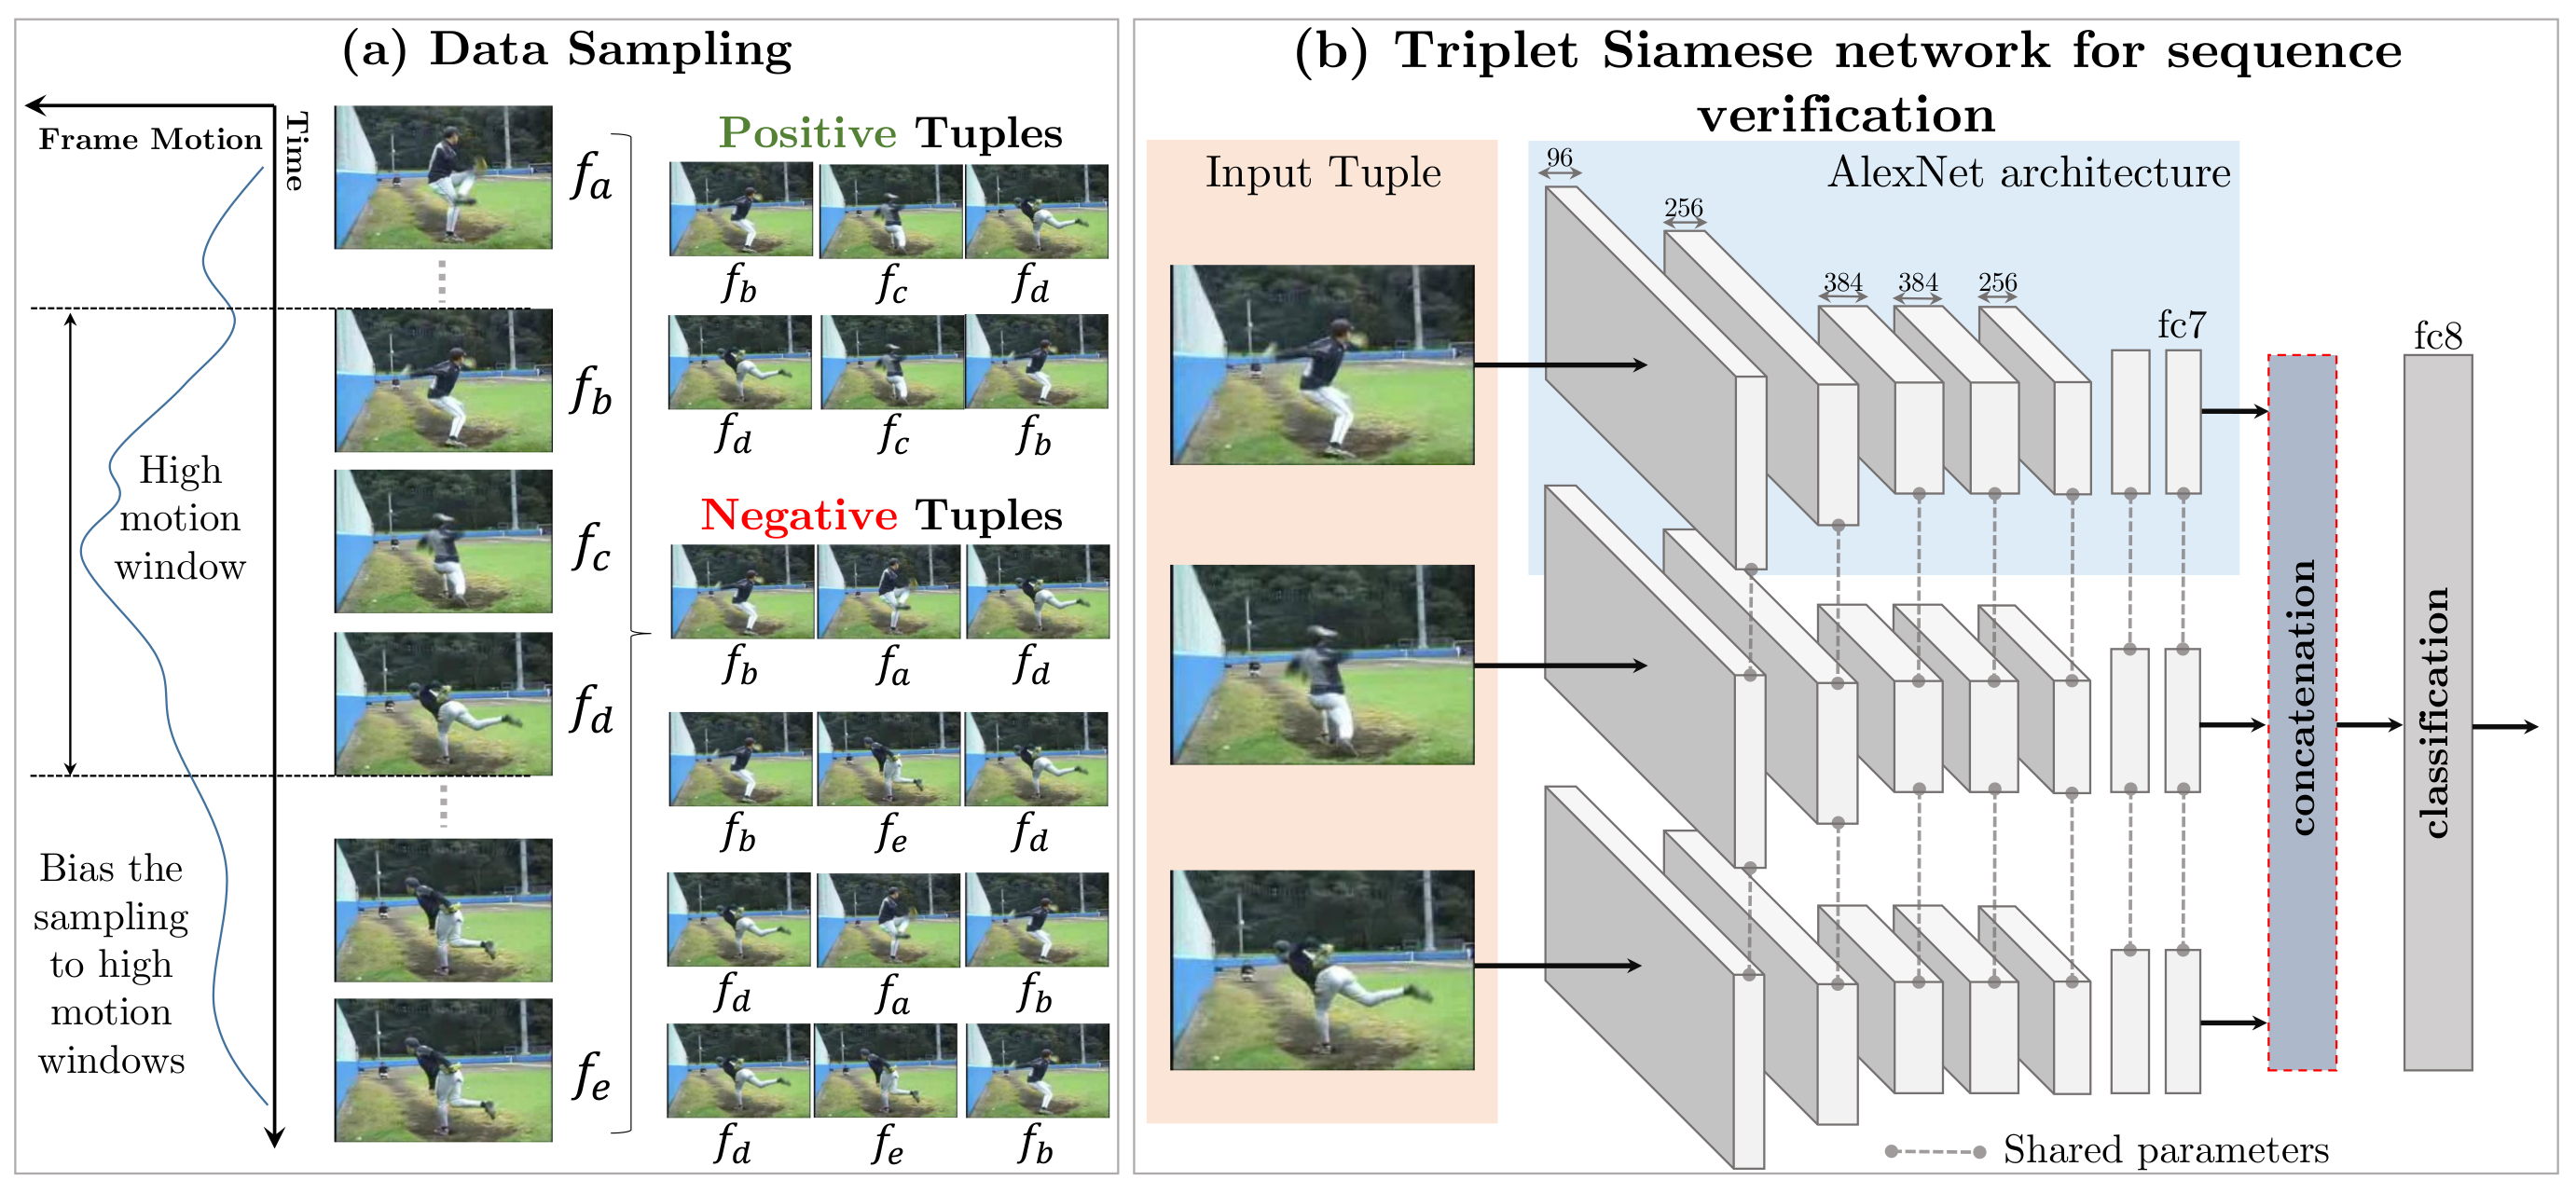
\includegraphics[width=\textwidth]{img_deep/shufflelearn_approach}
    \caption{Sampling method of input sequences and triplet Convolutional Neural Network for temporal order verification \cite{misra_shuffle_2016}}
    \label{fig:shufflelearn_approach}
\end{figure}

The three frames, that are used to construct positive and negative input sequences are sampled from regions in the video, which were previously identified to contain a certain magnitude of motion by using optical flow.
This ensures, that the sampled frames differ enough to make positive and negative sequences clearly distinguishable.

The authors use a CNN model called CaffeNet, which is a slightly modified version of AlexNet \cite{krizhevsky_imagenet_2012-1} and is publicly available in Caffe \cite{jia_caffe:_2014}. 
The CNNs form a siamese triplet, i.e.\ they all share the same parameters, and each one takes one of the frames of the sequence as input.
Each network maps its input frame to a high-level representation of activations in the layer $fc7$.
The three representations are concatenated an fed into a classifier for predicting, whether the sequence is in correct or not.

The network is trained on about $900$k sequences extracted from the training set of UCF-101 (split 1).
The resulting video representations can be reused for supervised action recognition training, by initializing the layers of a new CNN up to $fc7$ with the weights of the unsupervised model, adding an additional layer $fc8$ for the new task and fine-tuning the complete network using labeled training data.

To compare the advantage of their unsupervised pre-training method against no pre-training, the authors report results for the UCF-101 and HMDB-51 dataset (table \ref{tab:shufflelearn_results})

\begin{table}[H]
    \centering
    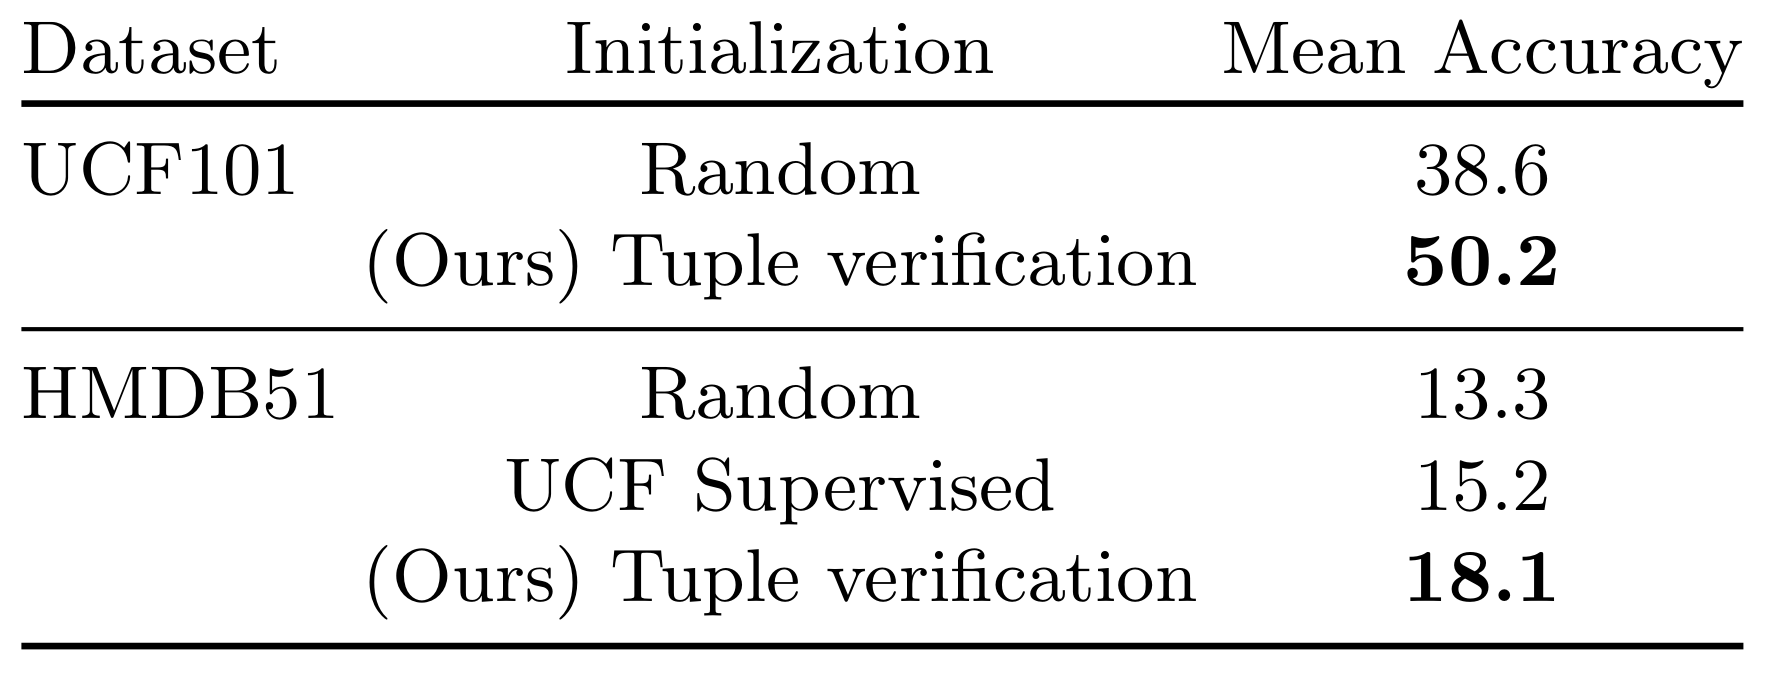
\includegraphics[width=0.5\textwidth]{img_deep/shufflelearn_results}
    \caption{Comparison of mean classification accuracies of a CaffeNet CNN with temporal order pre-training against without pre-training (random initialization of weights) on all three splits of UCF-101 and HMDB-51. \cite{misra_shuffle_2016}}
    \label{tab:shufflelearn_results}
\end{table}

On UCF-101 pre-training with temporal order verification yields a significant improvement of $+12.4\%$ against training the network from scratch.
On HMDB-51, the authors evaluate no pre-training, supervised pre-training on UCF-101 and pre-training using temporal oder verification.
The improvement of the latter is smaller compared to the results of UCF-101 but still significant (increase in mean accuracy of $+4.7\%$).
